\chapter{Analysis}
\label{chap:analysis}

\section{Search strategy}
\label{sec:strategy}

The strategy employed in this search is to define regions targeting both a high signal acceptance and purity, called signal regions (SRs). As indicated in \SectionRef{sec:BSM} and shown in~\FigureRef{fig:SvPSmedpt}, the expected shape of the signal varies according to the mediator mass and type ($\phi/a$), thus the strategy also aims to be as inclusive as possible in order to accommodate a wide range of potential signal \MET spectra. To this end, a categorization of the events passing the outlined selection criteria in \SectionRef{sec:selection} is performed based on the \mttll quantity defined in \SectionRef{subsec:mt2ll}. As alluded to earlier, the SM \ttll process is the most significant background for this search and by categorizing selected events according to whether the \mttll quantity is greater or less than 110\:\GeV, the discrimination power of the variable can be used to isolate a region highly enriched in the potential signal, as well as a less pure SR. Retaining events which comprise the low signal purity ($\mttll < 110\:\GeV$) category is meant to increase the sensitivity to potential signals with softer \MET spectra and correspondingly lower values of \mttll, despite the overwhelming dominance of SM \ttll in this category. The categorization is taken a step further and the events in each \mttll category are further split according to whether the leptons in the selected dilepton pair are the same or opposite flavor. Classifying the events based on SF vs OF changes the background composition of the categories, since almost no DY is expected in the case of the OF categories, while a far larger contribution is expected in the SF. The differing background composition as a result of the split into flavor regions also protects approximately half of the total search region from systematic uncertainties incurred only in the other half of the search region. Thus, events are separated into the following four SRs: high \mttll-SF, high \mttll-OF, low \mttll-SF, and low \mttll-OF. A potential signal observation would manifest as an excess over the expected \ptmiss from SM background processes, thus the signal extraction strategy is to perform a fit to the \ptmiss distribution. The \ptmiss distributions in each of the four SRs are fit simultaneously. This approach exploits the kinematic differences between the \ptmiss shapes of the \ttDM signals described in \ChapterRef{chap:signalsel} and the \ptmiss shapes of SM backgrounds detailed in \ChapterRef{chap:backgrounds}. The fitting procedure and statistical method is described later on in this chapter, in \SectionRef{sec:stats}.

\section{Data to simulation corrections}

Various corrections, in addition to the top \pt correction applied to the \ttll background only, are applied to the all processes estimated using simulation. The corrections account for mismodeling of distributions in the MC simulation, or to attempt to cover the difference between efficiencies measured in the data compared to those measured in the simulation. The corrections applied in this work are listed and described in the following section.

\subsection{Trigger efficiency}
\label{subsec:trigger}
The HLT triggers employed online to select potential dilepton events are a combination of dielectron, electron-muon, and dimuon triggers. In addition, single lepton triggers are used, but only approximately $4-6\%$ of the events passing the offline selection criteria as defined in~\SectionRef{sec:selection} are picked up by these. The suite of dilepton triggers make requirements on the lepton object reconstruction at the HLT level. As an example, the HLT trigger with the path name \texttt{HLT\_Ele23\_Ele12\_CaloIdL\_TrackIdL\_IsoVL\_DZ} is fired if an event contains two electrons with \pt thresholds above $23\:\GeV$ and $12\:\GeV$, and both electrons pass the loose working points for online electron identification from the calorimeters (\texttt{CaloIdL}), and the tracker (\texttt{TrackIdL}). The isolation requirement is very relaxed or ``very loose'' (\texttt{IsoVL}), and a quality requirement on the $|{d_{z}}|$ of the associated tracks to the PV is made (\texttt{DZ}). The following is a list of the dilepton triggers used:

\begin{itemize}
\item HLT\_Ele23\_Ele12\_CaloIdL\_TrackIdL\_IsoVL\_DZ
\item HLT\_Mu8\_TrkIsoVVL\_Ele23\_CaloIdL\_TrackIdL\_IsoVL
\item HLT\_Mu23\_TrkIsoVVL\_Ele12\_CaloIdL\_TrackIdL\_IsoVL
\item HLT\_Mu23\_TrkIsoVVL\_Ele12\_CaloIdL\_TrackIdL\_IsoVL\_DZ
\item HLT\_Mu17\_TrkIsoVVL\_Mu8\_TrkIsoVVL
\item HLT\_Mu17\_TrkIsoVVL\_Mu8\_TrkIsoVVL\_DZ
\item HLT\_Mu17\_TrkIsoVVL\_TrkMu8\_TrkIsoVVL\_DZ
\end{itemize}
 
The efficiencies of each lepton ``leg'' of the triggers listed is measured in the data and simulation using a method standard to experimental particle physics, generically called the ``Tag and Probe'' method. In this work, the method exploits dilepton resonances, such as $Z\rightarrow\ell\ell$ events for the $ee$ and $\mu\mu$ measurements, and dileptonic \ttll decays for the $e\mu$ measurements. In this case, a ``tag'' electron is required to fire a single electron trigger and pass the ``Tight'' working point as outlined in \TableRef{tab:ele_wp}, and have a $\pt>40\:\GeV$ and $|\eta|<2.1$, for the efficiency measurements of the $ee$ trigger and $\mu$-leg of the $e\mu$ trigger. A ``tag'' muon is required to fire a single muon trigger and pass the ``Tight'' working point criteria as outlined in \TableRef{tab:muon_wp} and have a $\pt>30\:\GeV$, for the efficiency measurements of the $\mu\mu$ trigger and $e$-leg of the $e\mu$ trigger. Subesequently, the ``probe'' is the other lepton in the event and is termed as ``passing''/``failing'' if the trigger leg in question for which the efficiency is being measured has/has not been fired by the lepton. Orthogonal samples of ``tag + passing probe'' and ``tag + failing probe'' are then obtained and the efficiency is computed as a ratio of the former category to the sum of the two categories. The efficiencies are measured in data and simulation and are parametrized in both lepton $\pt$ and $|\eta|$, where the scale factor applied to the simulation is the ratio of the data to simulation efficiencies. \FigureRef{fig:mueg_sf} shows the scale factors derived for the electron and muon legs of the muon-electron trigger, where the scale factors are nearly unitary though a lower efficiency is observed for the electron leg for low \pt electrons with $2.1<\eta<2.4$ in data than in the simulation. The correction is then applied to the simulation as,

\begin{equation}
 \frac{ {\Big[\epsilon_{\ell1}\cdot\epsilon_{\ell2}\cdot\:f + (1-f)\Big]}_\text{data}}{ {\Big[\epsilon_{\ell1}\cdot\epsilon_{\ell2}\cdot\:f + (1-f)\Big]}_\text{MC}},  
\end{equation} 

where $\epsilon_{\ell1/\ell2}$ denotes the double lepton trigger efficiency of either lepton leg as measured, and $f$ denotes the approximate fraction of events triggered on using the double lepton triggers as measured in data and simulation.

\begin{figure}
\begin{center} 
    \subfloat[][$e\mu$ trigger: $e$ leg]  {\label{subfig:ele_SF_MuEG}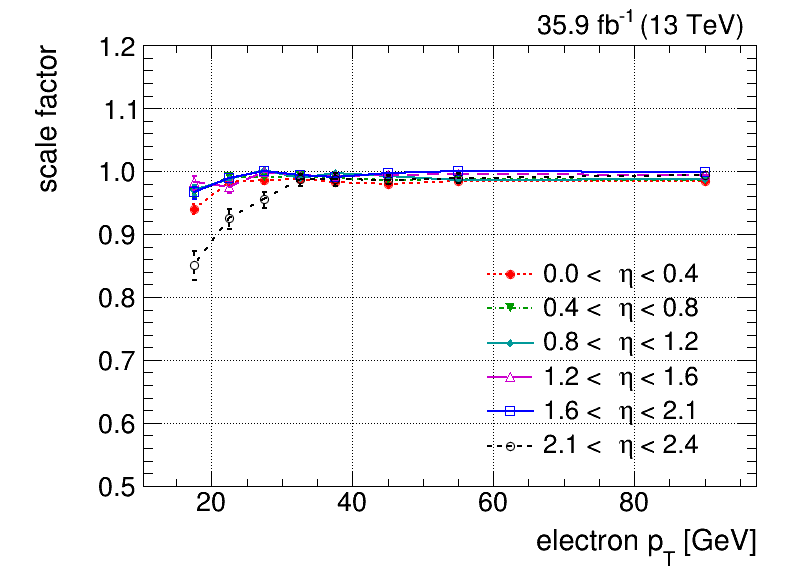
\includegraphics[width=0.48\textwidth]{figs/ele_mueg_sfetapt.png}}
    \subfloat[][$e\mu$ trigger: $\mu$ leg]{\label{subfig:mu_SF_MuEG}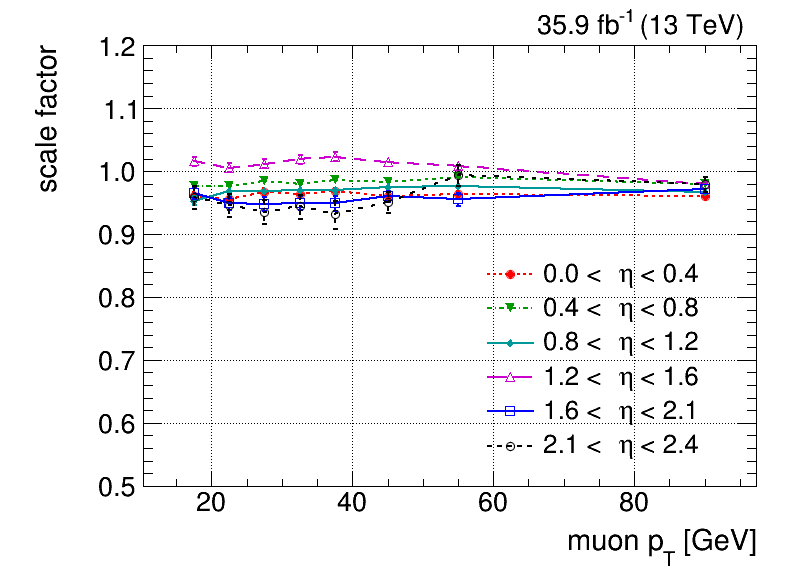
\includegraphics[width=0.48\textwidth]{figs/mu_mueg_sfetapt.png}}
    \caption{Scale factors for the electron and muon leg of the muon-electron trigger parametrized in lepton $\pt$ and $\eta$.}
    \label{fig:mueg_sf}
  \end{center}
\end{figure}

\subsection{PU reweighting}
\label{subsec:pu}
The simulation does not reproduce the PU distribution as observed in the data, so in order to alleviate this discrepancy, the simulation is re-weighted to the estimated PU distribution in data. The re-weighting is derived from the measured instantaneous luminosity of the bunch crossings during the 2016 pp collision data-taking period and the estimated total inelastic cross section. The cross section is estimated using minimum bias (MB) events. In the experimental sense, a MB event is one which has been triggered on as a result of minimum detector activity and in the theoretical sense, MB triggers target non-single diffractive inelastic interactions. The total pp cross section, $\sigma_\mathrm{tot}$ is comprised of,

\begin{equation}
  \sigma_{\mathrm{tot}} = \sigma_{\mathrm{elas}} + \sigma_{\mathrm{SD}} + \sigma_{\mathrm{DD}} + \sigma_{\mathrm{ND}} + \sigma_{\mathrm{CD}}
  \label{eq:totppxsec}
\end{equation}

where from left to right, the terms on the right-hand side of Eq.~\ref{eq:totppxsec} correspond to contributions to the cross section from elastic scattering, single diffractive dissociation, double diffractive dissociation, non-diffractive inelastic scattering, and central diffractive dissociation. In a more accurate sense, MB events are covered by the $\sigma_{\mathrm{DD}}$ and $\sigma_{\mathrm{ND}}$ terms. The cross section estimate for 2016 data-taking is 69.2 mb for MB events, with an uncertainty of $4.6\%$. The ratio of normalized distributions of the number of PU interactions in data and \ttll simulation is used to extract the scale factors that are applied to the simulation on an event-by-event basis. The PU profiles in data and simulation are shown in~\FigureRef{fig:pu}, where the simulation is also shown with the MB cross section varied by $\pm4.6\%$ in~\FigureRef{subfig:pileup-unc}. The effect of the PU re-weighting can be seen in~\FigureRef{fig:npv}, where the distribution of the number of reconstructed primary vertices (PV) is shown before and after the re-weighting. Discrepancies between the data and the simulation still exist in the $\text{N}_{PV}$ distribution, however this search is not strongly reliant on the modeling of the number of PV or PU interactions. In addition, the effects of such discrepancies are taken into account and treated as a systematic uncertainty in the final fit, to be described later. 

\begin{figure}
  \subfloat[][]{\label{subfig:pileup}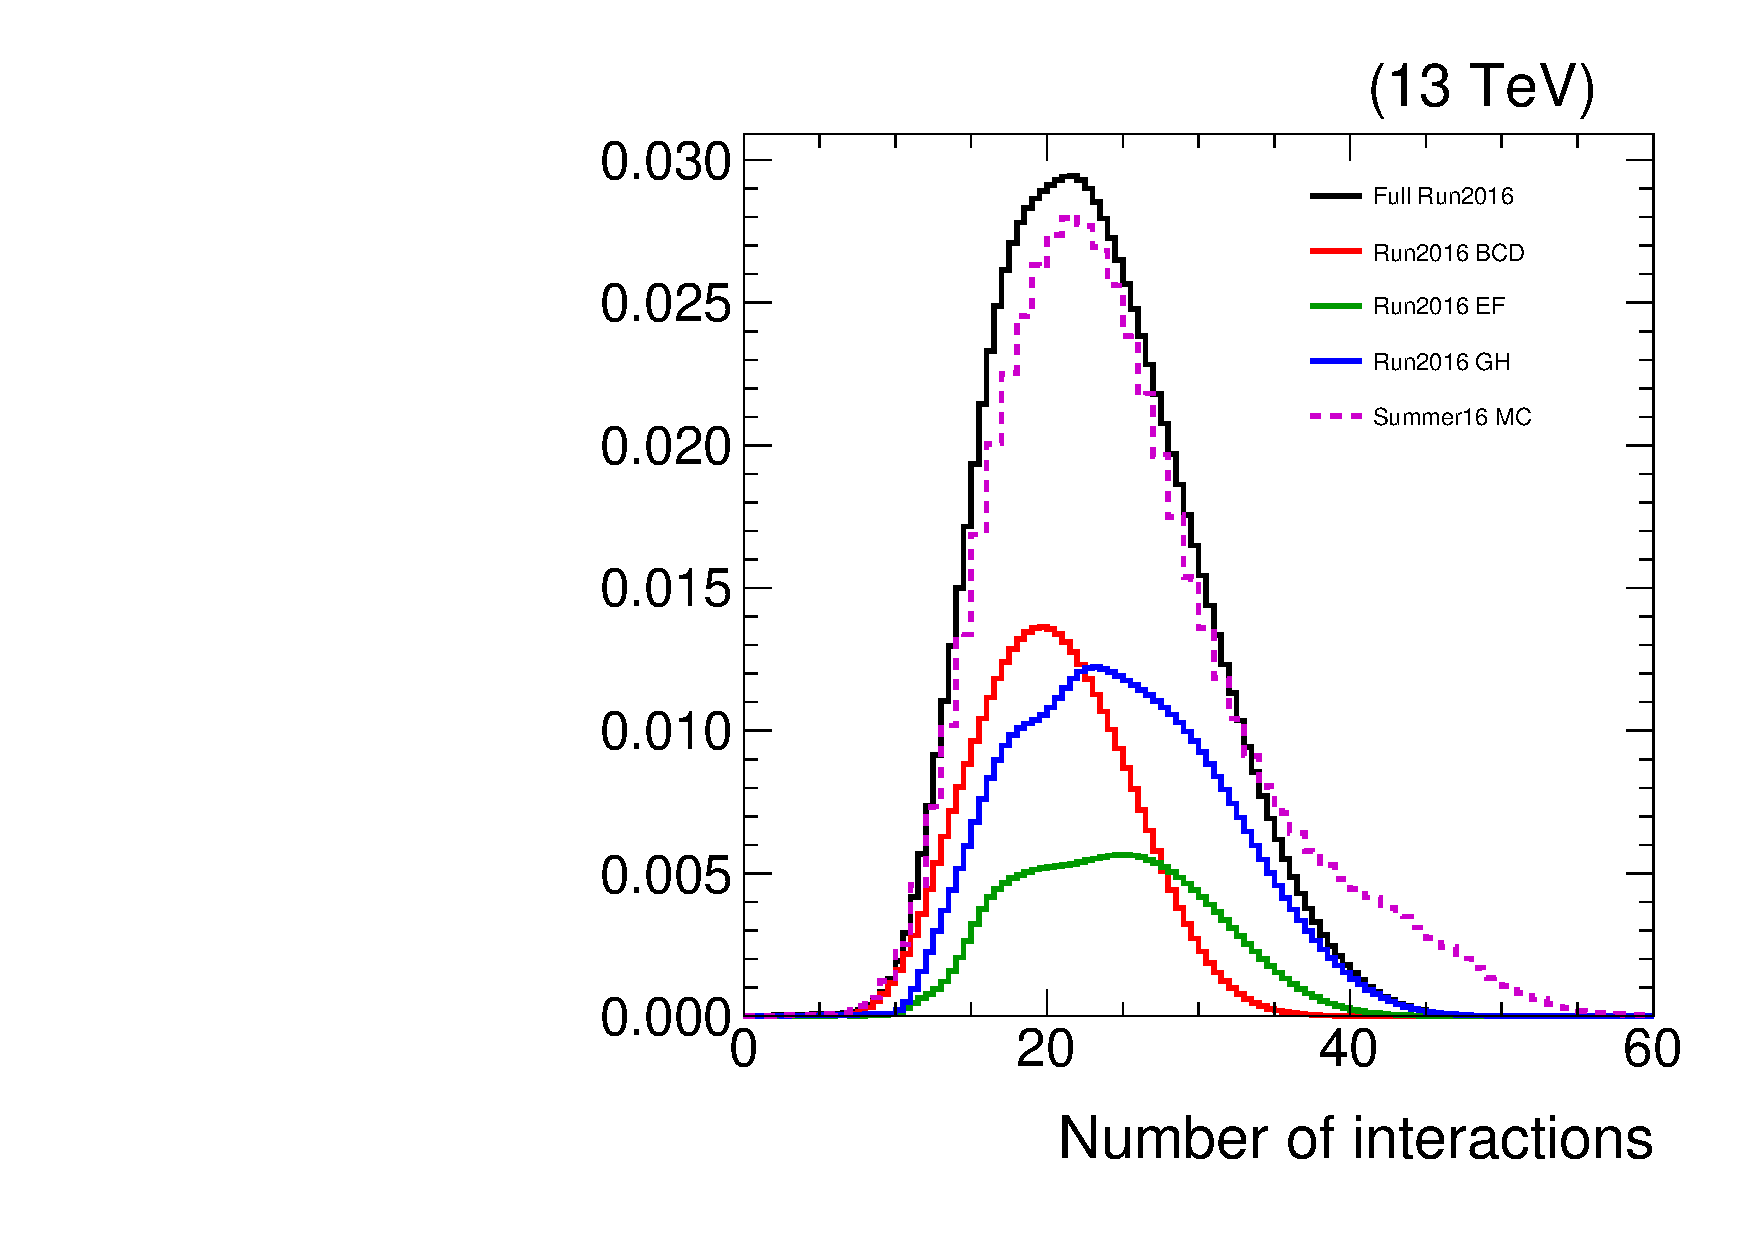
\includegraphics[width=0.48\textwidth]{figs/pileup.pdf}}
  \subfloat[][]{\label{subfig:pileup-unc}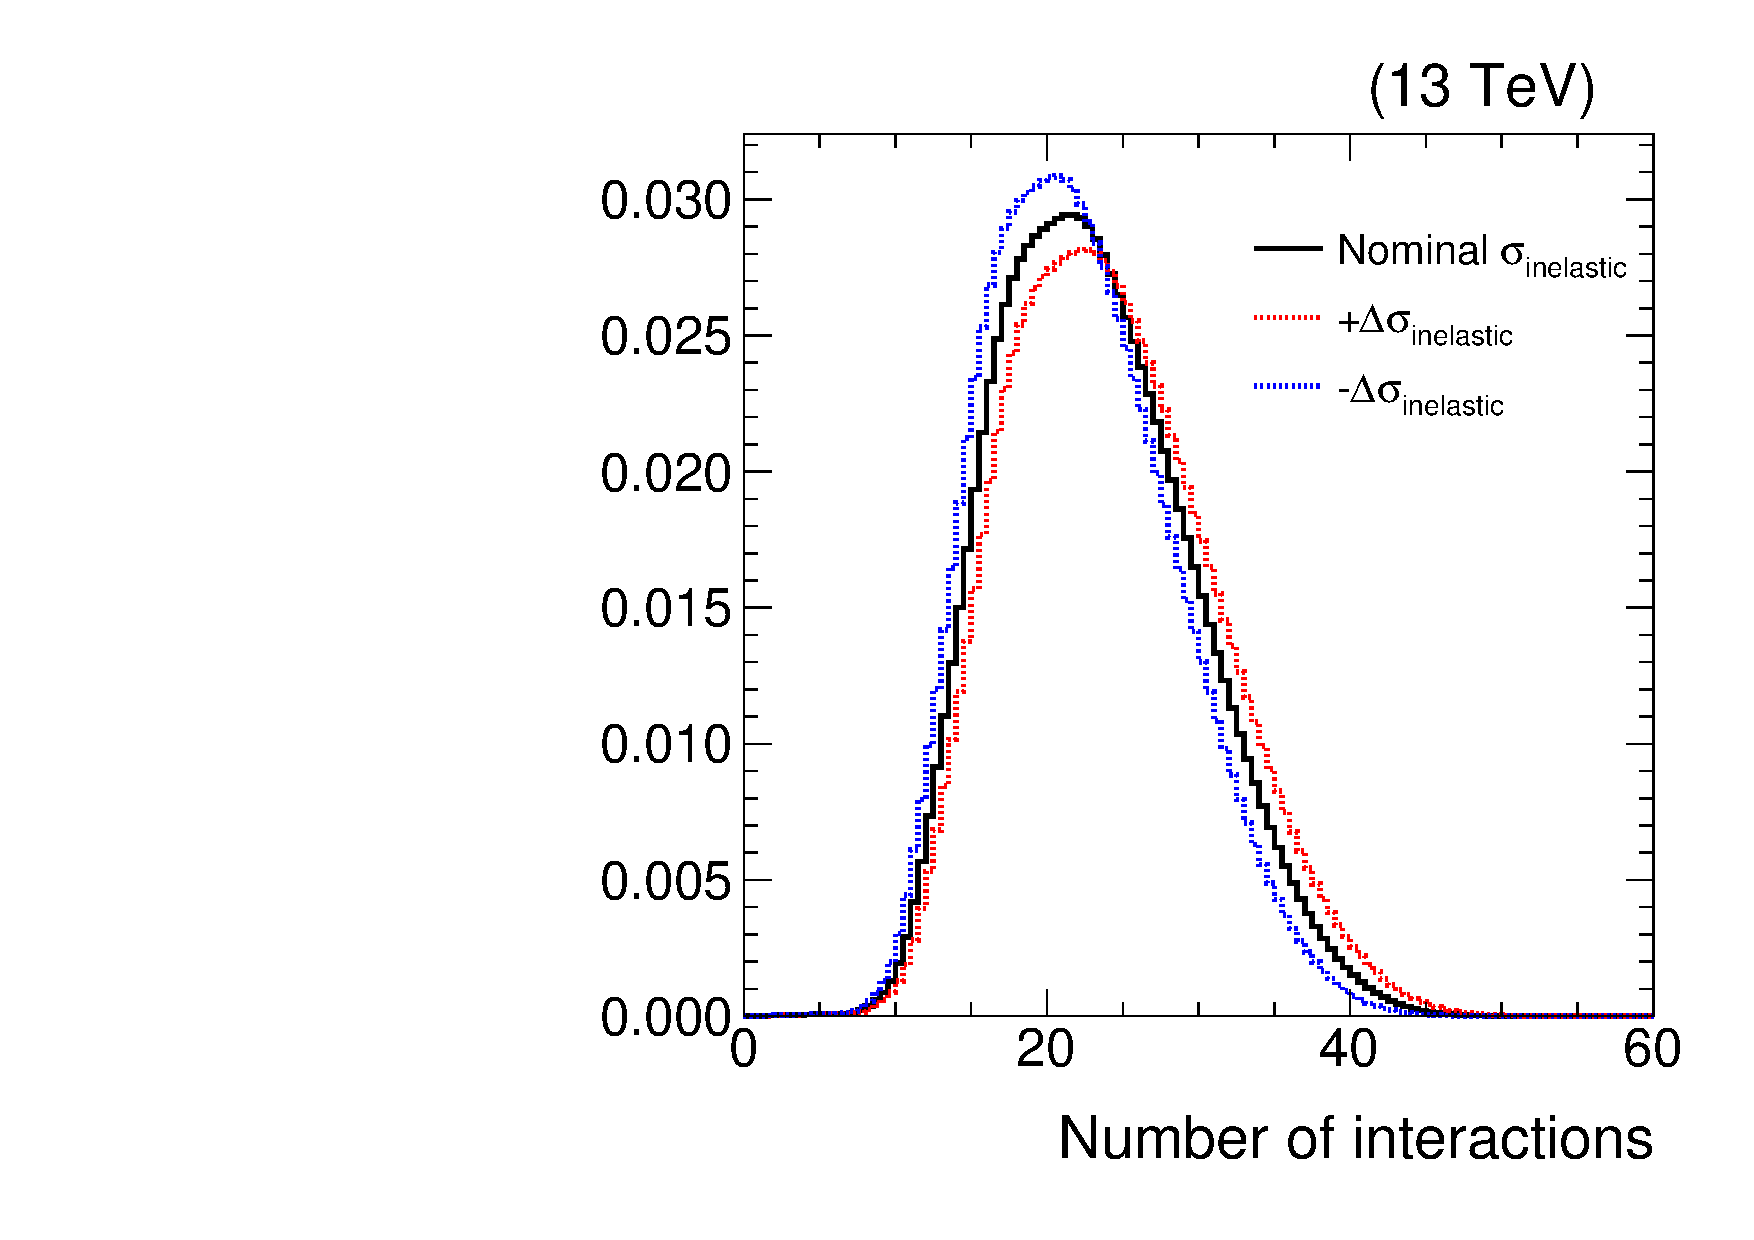
\includegraphics[width=0.48\textwidth]{figs/pileup-unc.pdf}}
  \caption{\protect\subref{subfig:pileup} Pileup distributions in data and MC. Also shown are the pileup profiles in a few run ranges scaled to the relative contribution to the total integrated luminosity.\protect\subref{subfig:pileup-unc} The pileup distributions from varying the total inelastic cross section by $\pm4.6\%$.}
  \label{fig:pu}
\end{figure}

\begin{figure}
  \subfloat[][]{\label{subfig:npvPRE}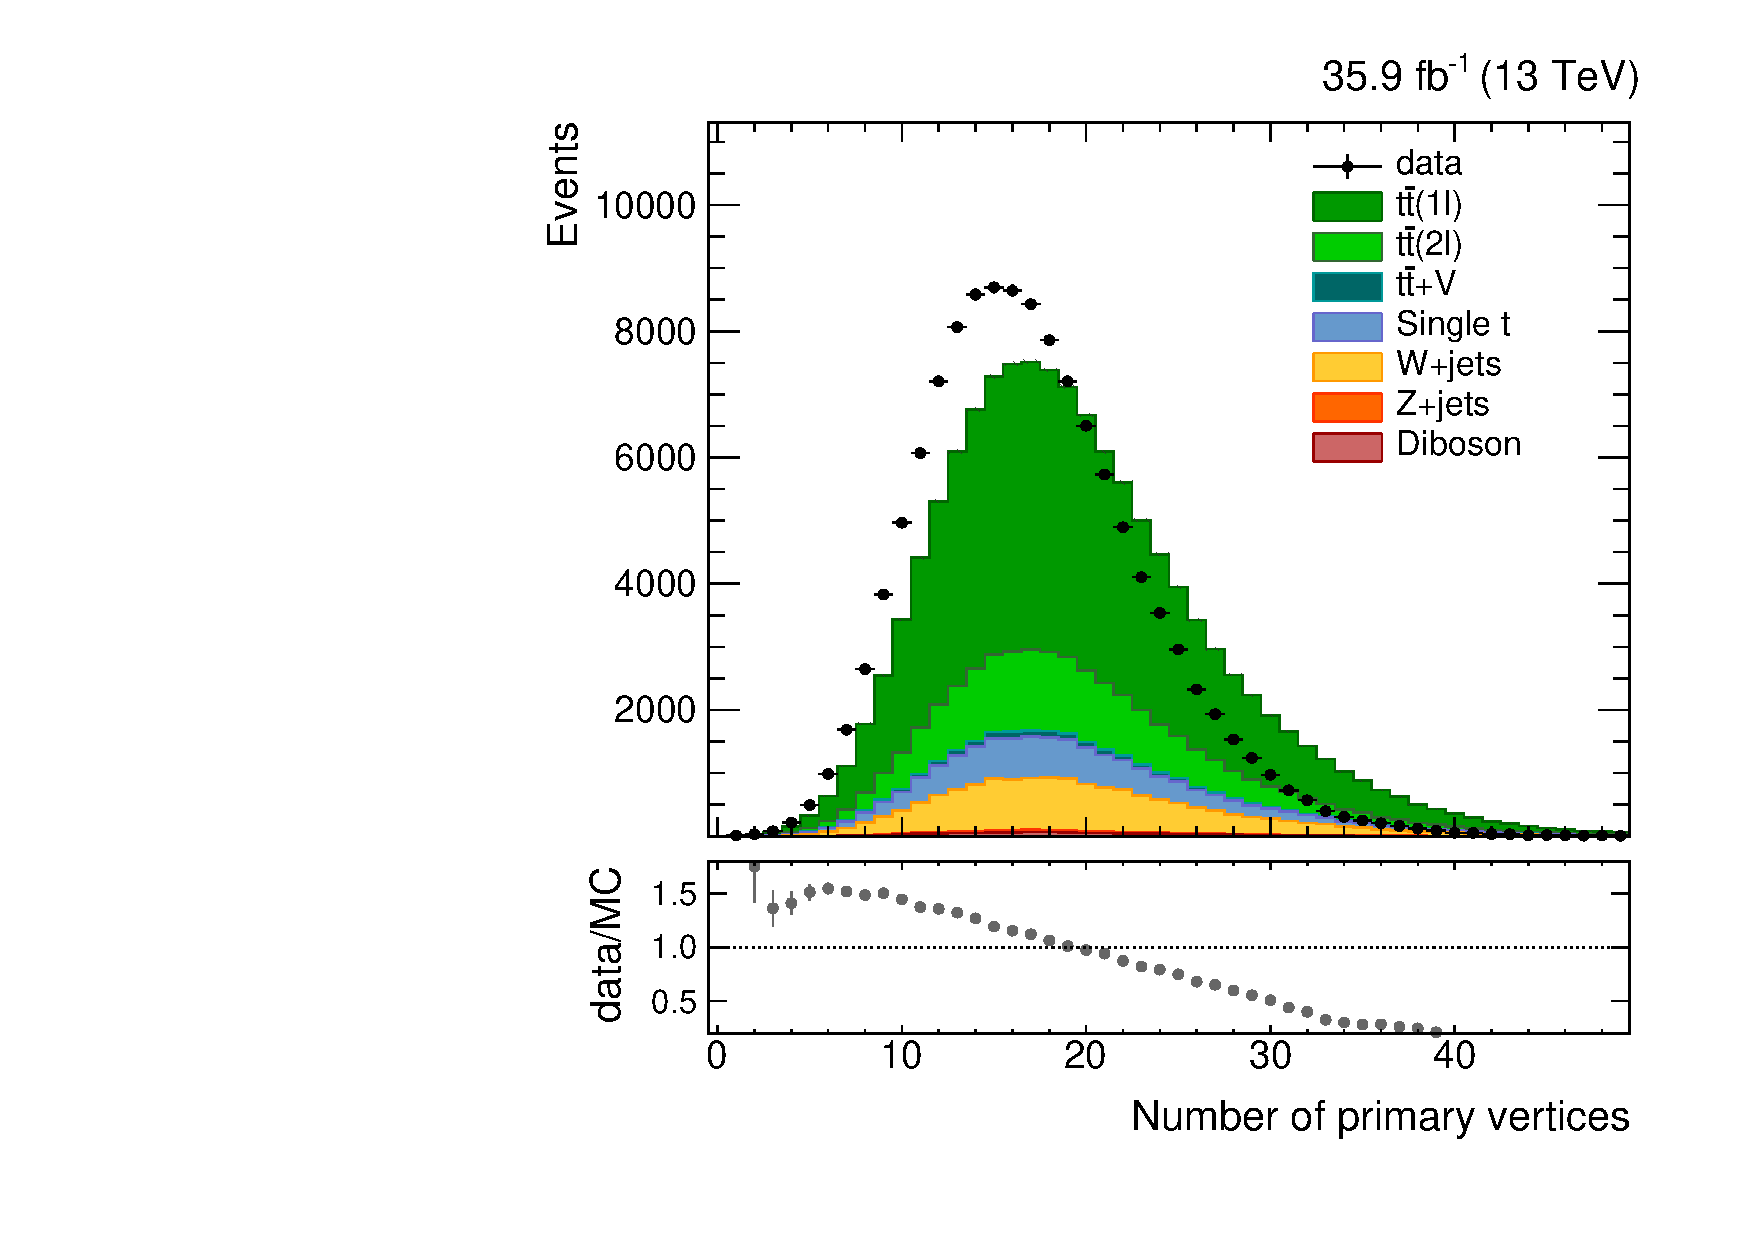
\includegraphics[width=0.48\textwidth]{figs/npv_pre.pdf}}
  \subfloat[][]{\label{subfig:npvPOST}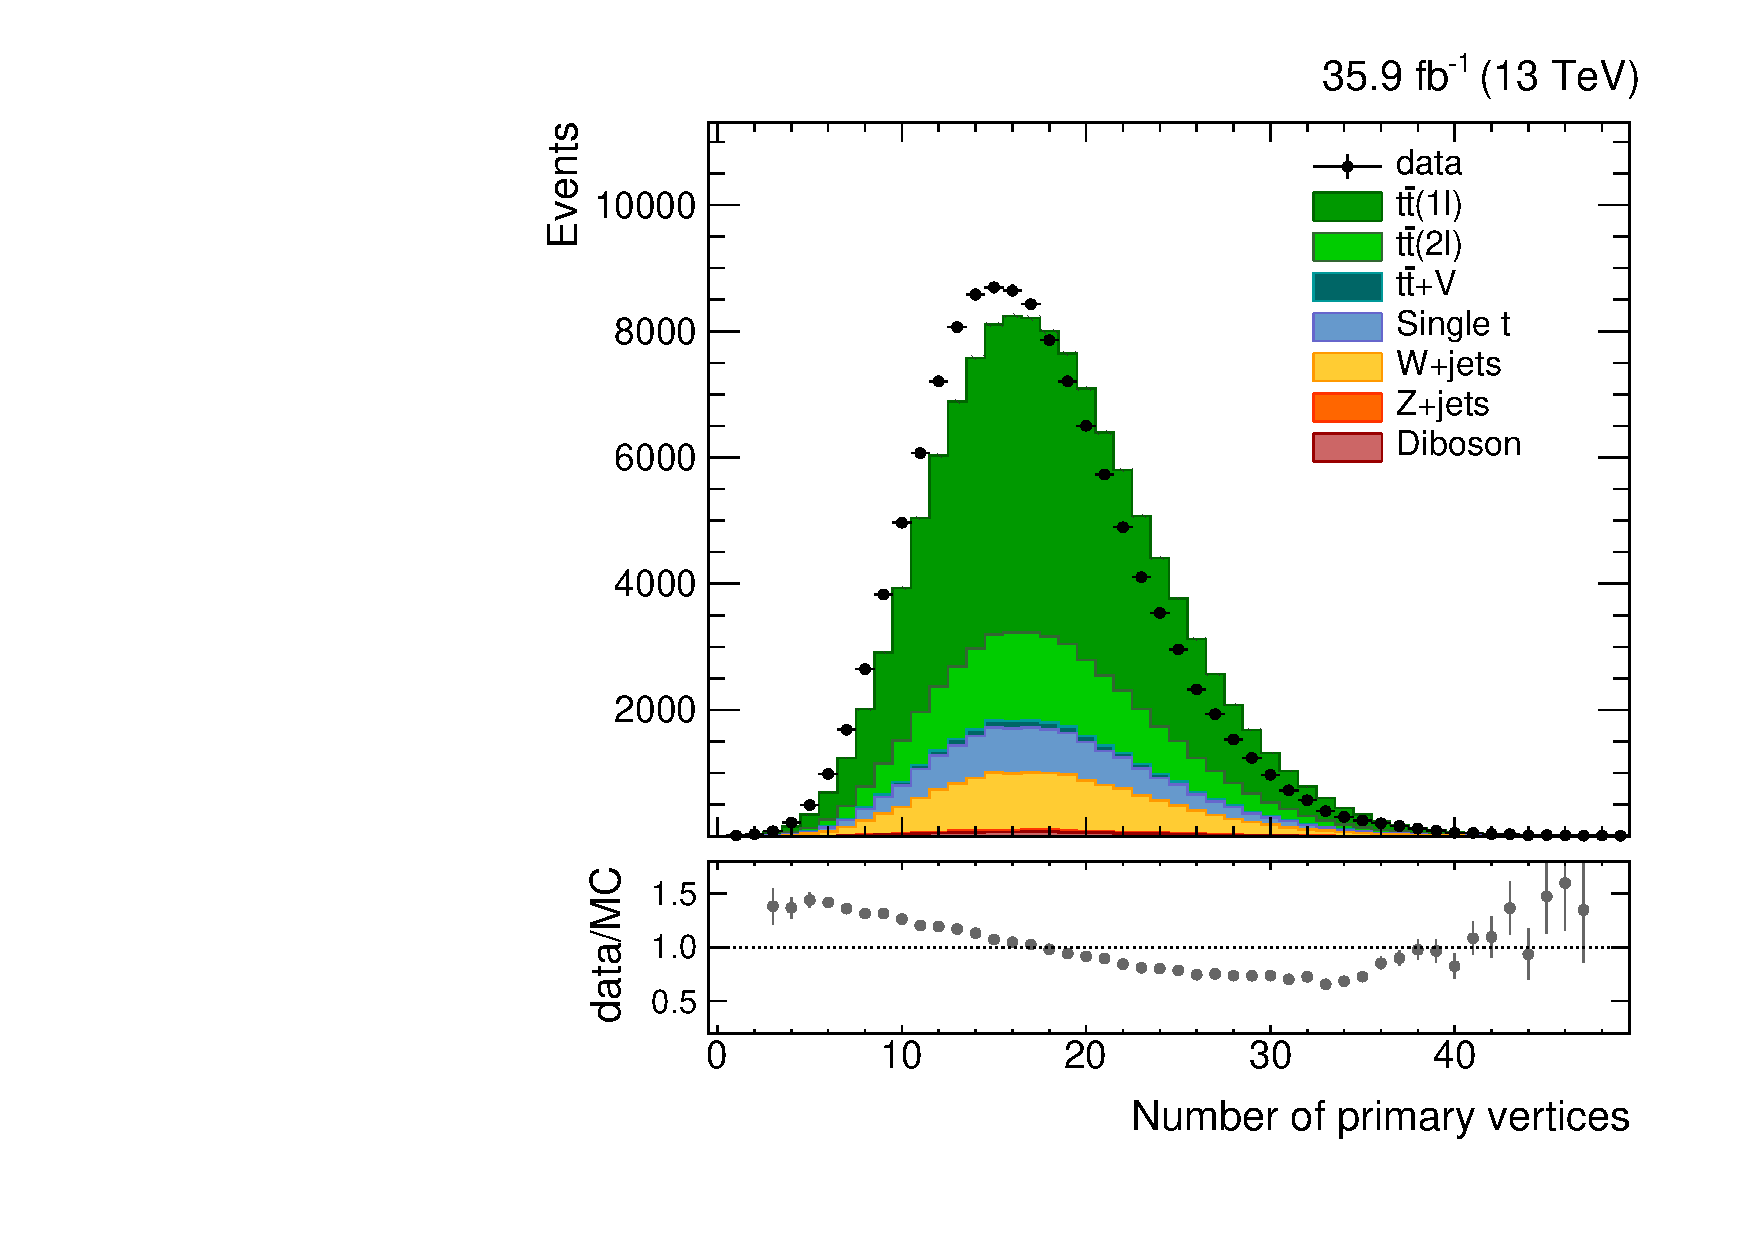
\includegraphics[width=0.48\textwidth]{figs/npv_post.pdf}}
  \caption{$\text{N}_{PV}$ distributions in data and MC pre and post PU re-weighting in a region dominated by semileptonic \ttbar events. The MC is normalized to the observed yield.}
  \label{fig:npv}
\end{figure} 

\subsection{b-tagging efficiency}

The efficiency to tag jets orginating from b-quark hadronization is dependent on the working point of the b-tagging algorithm used (in this case the CSV algorithm as defined in \SectionRef{subsec:btag}), and the jet kinematics in the signal region of interest. Hence, the performance is characterized based on the probabilities to correctly tag a b jet ($\epsilon_{b}$), to misidentify the hadronization of a c-quark as a b jet ($\epsilon_{c}$), and to misidentify light flavor or gluon initiated jets as b jets ($\epsilon_{udsg}$). Each efficiency is defined by,

\begin{equation}
  \epsilon_{f}(\pt,\eta) = \frac{N_{f}^{\text{b-tagged}}(\pt,\eta)}{N_{f}^{\text{Total}}(\pt,\eta)}, f=b,c,udsg
\end{equation}

where the efficiency is determined in bins of jet \pt and \eta, and $N_{f}^{\text{Total}}$ and $N_{f}^{\textrm{b-tagged}}$ are the total number of jets and the number of b-tagged jets of flavor $f$. 

\begin{figure}
  \subfloat[][]{\label{subfig:beff}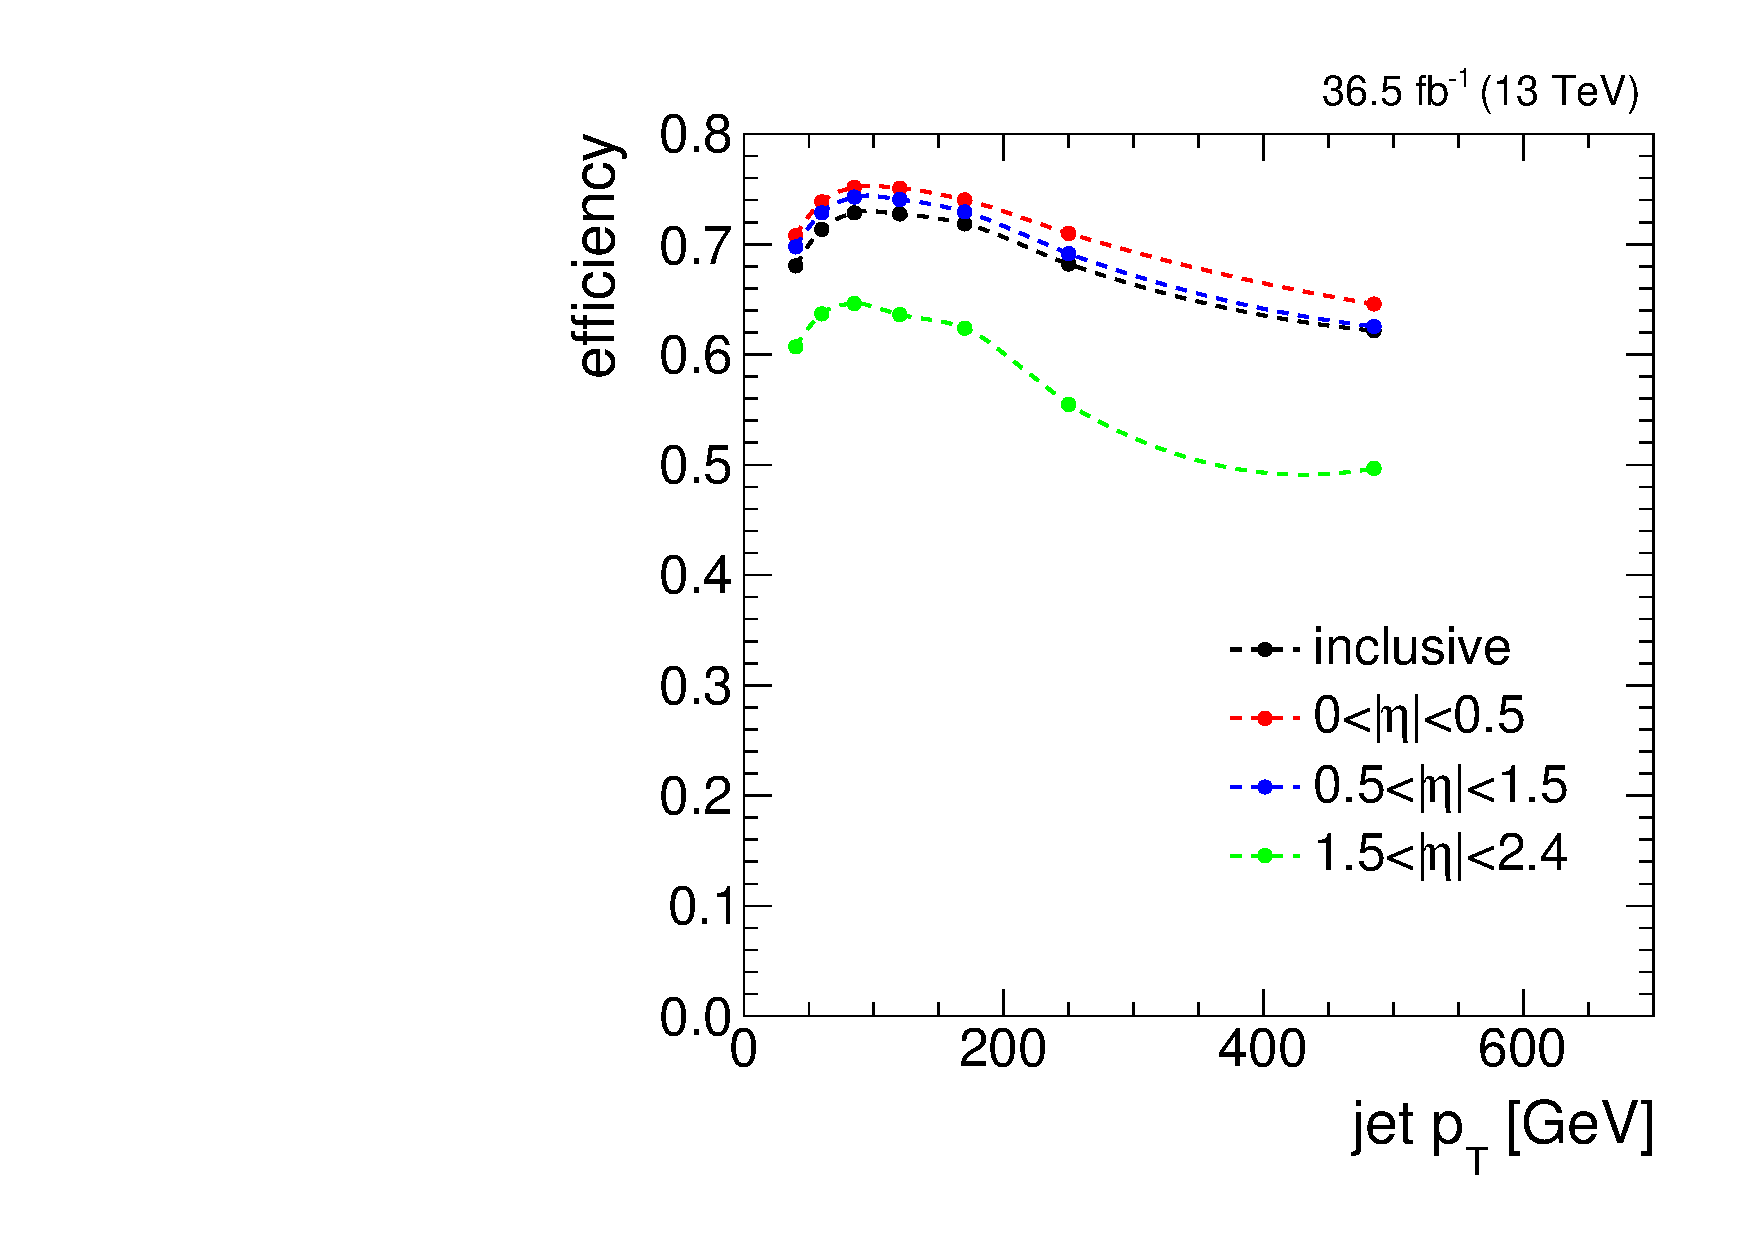
\includegraphics[width=0.48\textwidth]{figs/b_effpt.pdf}}
  \subfloat[][]{\label{subfig:ceff}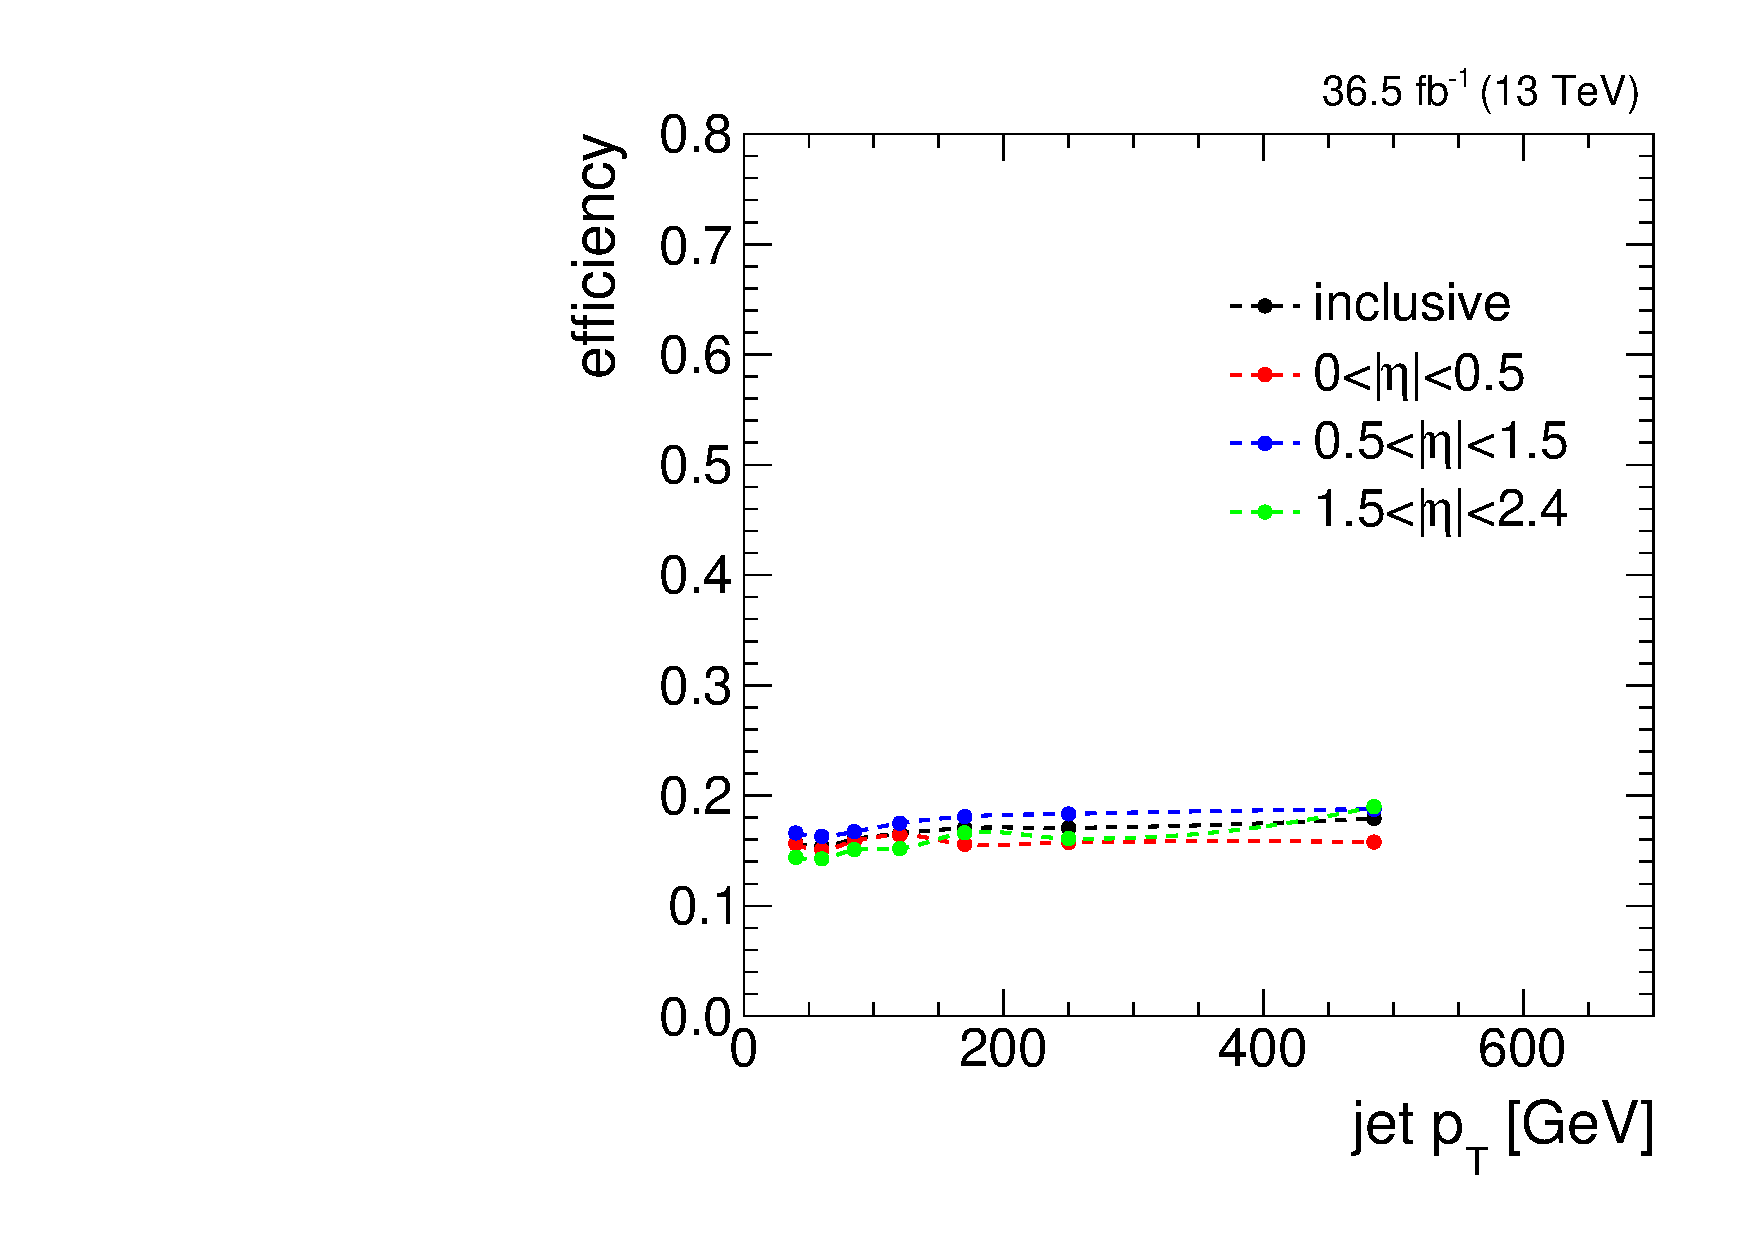
\includegraphics[width=0.48\textwidth]{figs/c_effpt.pdf}}\\
  \subfloat[][]{\label{subfig:leff}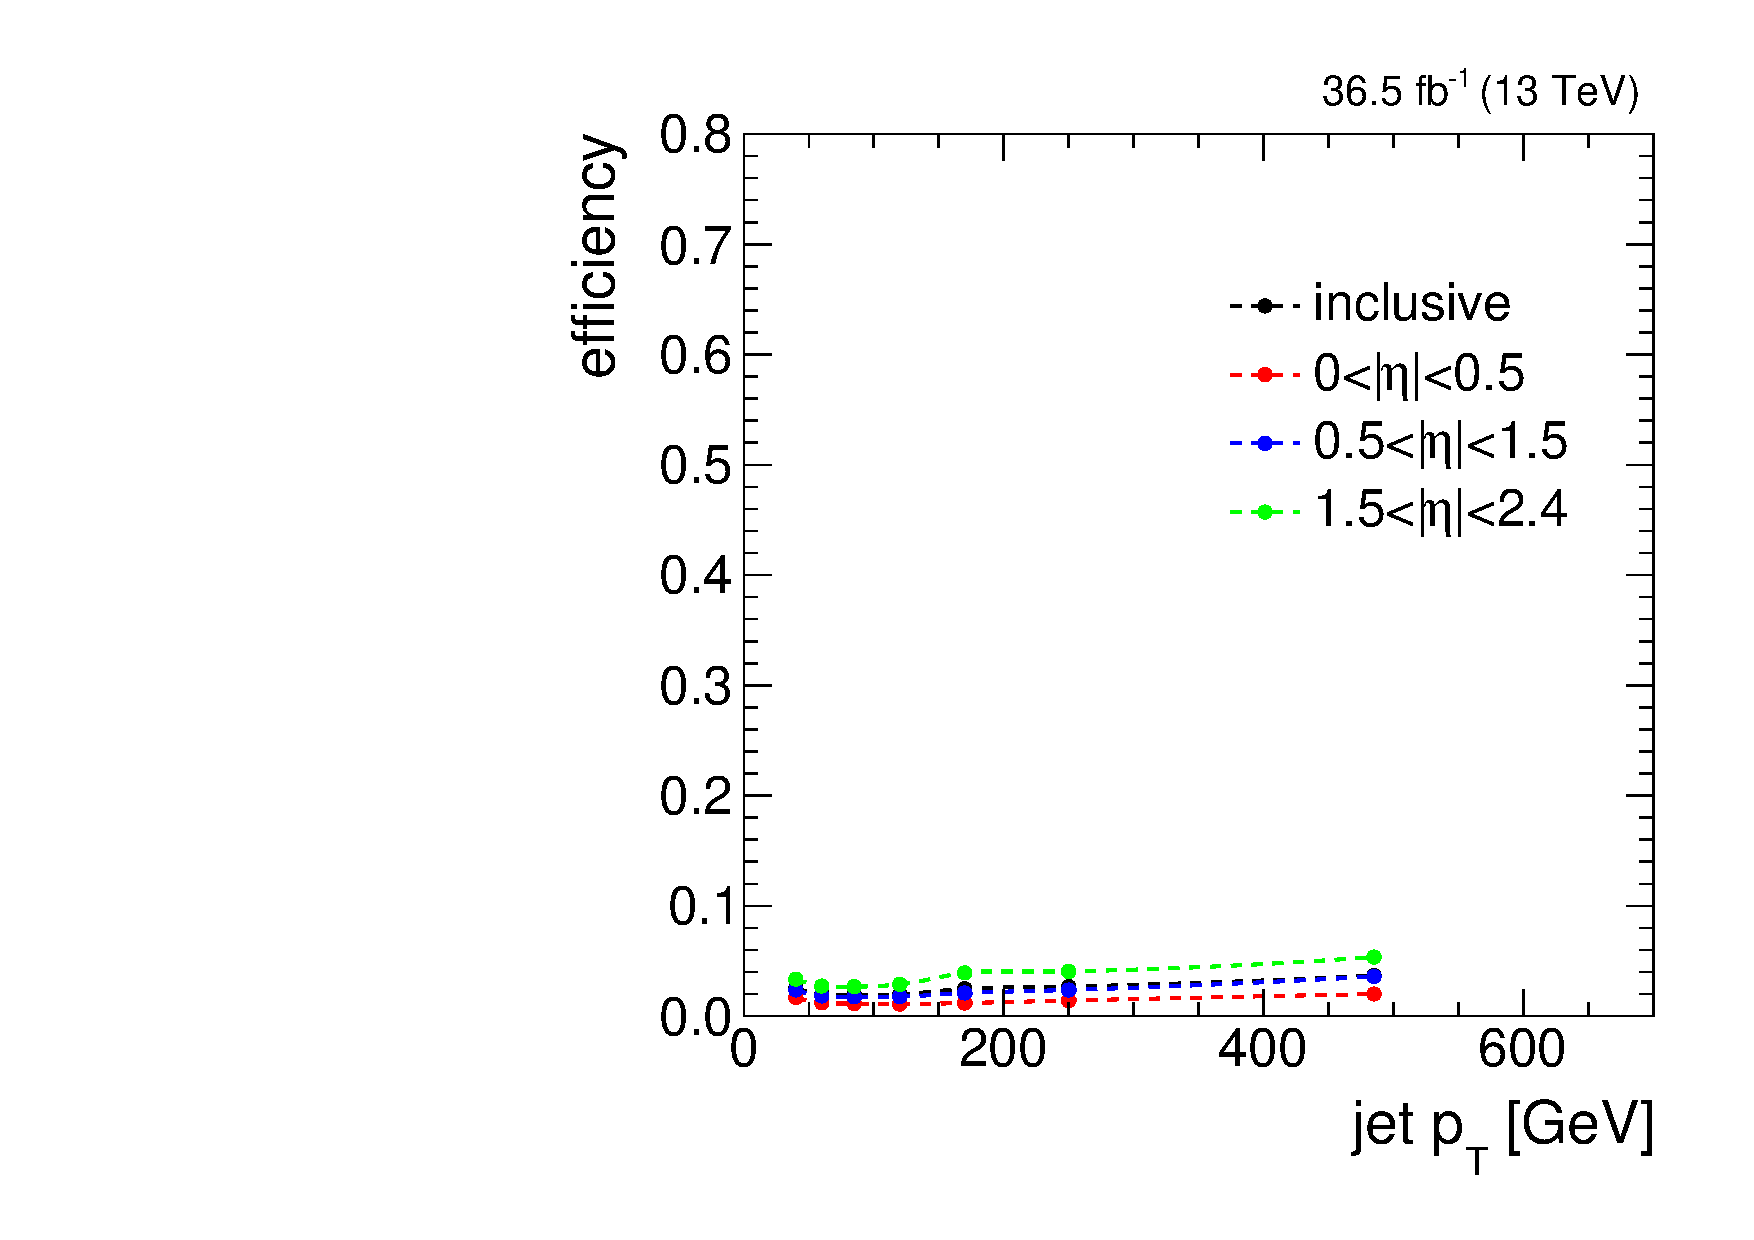
\includegraphics[width=0.48\textwidth]{figs/l_effpt.pdf}}
  \caption{The efficiency in \ttll simulation is measured as a function of jet \pt and various \eta bins for~\protect\subref{subfig:beff} correctly tagging b jets,~\protect\subref{subfig:ceff} misidentifying c jets,~\protect\subref{subfig:leff} and misidentifying light flavor or gluon jets.}
  \label{fig:btageff}
\end{figure}

The CSV algorithm has three working points which correspond to different values of $\epsilon_{udsg}$ as measured in data. They are defined as loose ($\epsilon_{udsg}=~10\%$), medium ($\epsilon_{udsg}=~1\%$), and tight ($\epsilon_{udsg}=~0.1\%$). In the following analysis, the medium working point is used and corresponds to a b-tagging efficiency of $\epsilon_{b}=69\%$, and an c-jet mistag efficiency of $\epsilon_{c}=35\%$ in data. The efficiency of the medium working point is measured in a simulation sample of dilepton \ttbar and shown in~\FigureRef{fig:btageff} for each jet flavor as a funtion of \pt and \eta. In general, the more central a jet is within the detector volume (corresponding to smaller $|\eta|$), the higher the b-tagging efficiency and lower the mistag rate is expected to be. As can be understood from~\FigureRef{subfig:beff}, although the efficiency in the highest \eta bin ranges from 0.62 to 0.5 for low to high jet \pt values, the inclusive efficiency lies at approximately 0.7 demonstrating that most of the selected b-jets are central. 

The corrections are applied in an event-by-event method, where the b-tagging combinatorics are also accounted for. For every selected jet in the event, the probability that it is correctly tagged or mis-tagged depending on flavor is $\epsilon^{\text{tag}}$ and $(1-\epsilon^{\text{tag}})$, respectively. If no b-tagged jets are expected, the corresponding event efficiency is then,

\begin{equation}
  \epsilon_{\text{event}} = \prod_{i=\text{\# jets}} (1-\epsilon^{\text{tag}}_i).
  \label{eq:0btag}
\end{equation}

The signal region selection stipulates that events must contain at least one b-tagged jet, so it follows that the event efficiency is defined as the ``inverse'' of Eq.~\ref{eq:0btag}, such that,

\begin{equation}
  \epsilon_{\text{event}} = 1 - \prod_{i=\text{\# jets}} (1-\epsilon^{\text{tag}}_i).
  \label{eq:more0btag}
\end{equation}

The corrections are applied to the simulation based on the ratio of the event efficiencies measured in the data and simulation, $\text{SF}_\text{b-tag} = \frac{\epsilon_{event}^{\text{data}}}{\epsilon_{event}^{\text{MC}}}$, in order to cover any differences in efficiency with respect to the performance in data.

\section{Discriminating observables}
\label{sec:observables}

\ptmiss is the detector observable which provides the strongest discrimination between the \ttDM signal and the dominant SM dileptonic \ttbar background. In addition to the main observable used for the signal extraction, multiple other observables are scrutinized as a means to ascertain that significant discrepancies between the data and the simulation are not present in the signal region. These can be seen in the same flavor and opposite flavor channels, respectively, in ~\FigureRef{fig:dilep_sr_sf} and ~\FigureRef{fig:dilep_sr_em}. The observables include the multiplicity of jets ($N_{\textrm{jets}}$), and that of b-tagged jets ($N_{\text{b-jets}}$), as well as kinematic distributions for the highest \pt (leading) lepton and jet in the event. Variables which combine the kinematic information from the two leptons in the event such as the \pt and mass of the dilepton system, $\pt^{\ell\ell}$ and $m_{\ell\ell}$ are presented. %The azimuthal separation between the dilepton system and the \ptvecmiss, $\Delta\phi(\vec{p}_{\text{T}}^{\ell\ell},\ptvecmiss)$, is also shown, along with the uncategorized \ptmiss spectrum.

The \mttll distribution used to categorize events into a low ($\mttll<110\:\GeV$) and high ($\mttll>110\:\GeV$) signal purity category is shown in ~\FigureRef{fig:mt2_sr}. The subsequent \ptmiss spectra in the low and high purity signal regions are shown in ~\FigureRef{fig:metlo} and ~\FigureRef{fig:methi}, respectively. 

\begin{figure}
  \centering
  \subfloat[$N_{\textrm{jets}}$]   {\label{subfig:njets_sf}    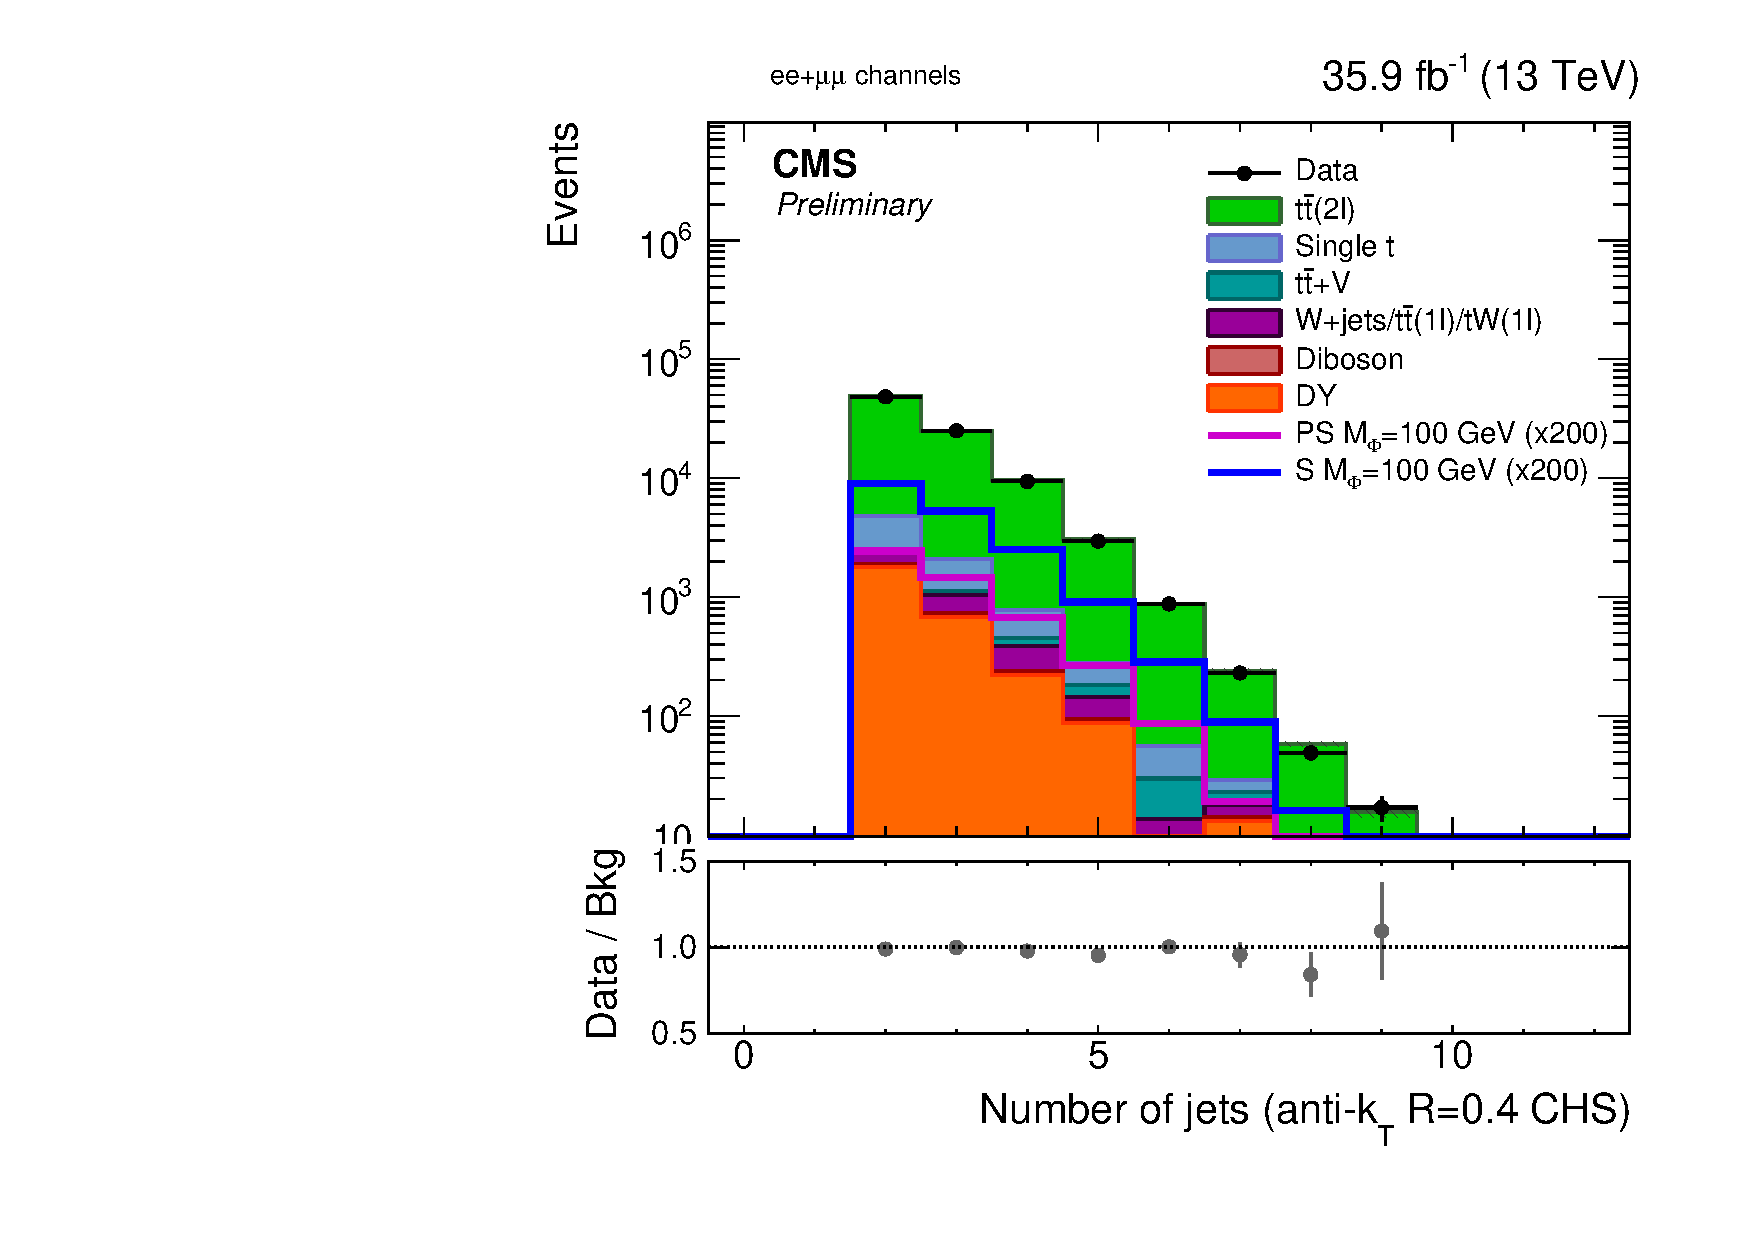
\includegraphics[width=0.4\textwidth]{figs/inclusiveSR/njets_sf.pdf}}
  \subfloat[$N_{\textrm{b-jets}}$] {\label{subfig:nbjets_sf}   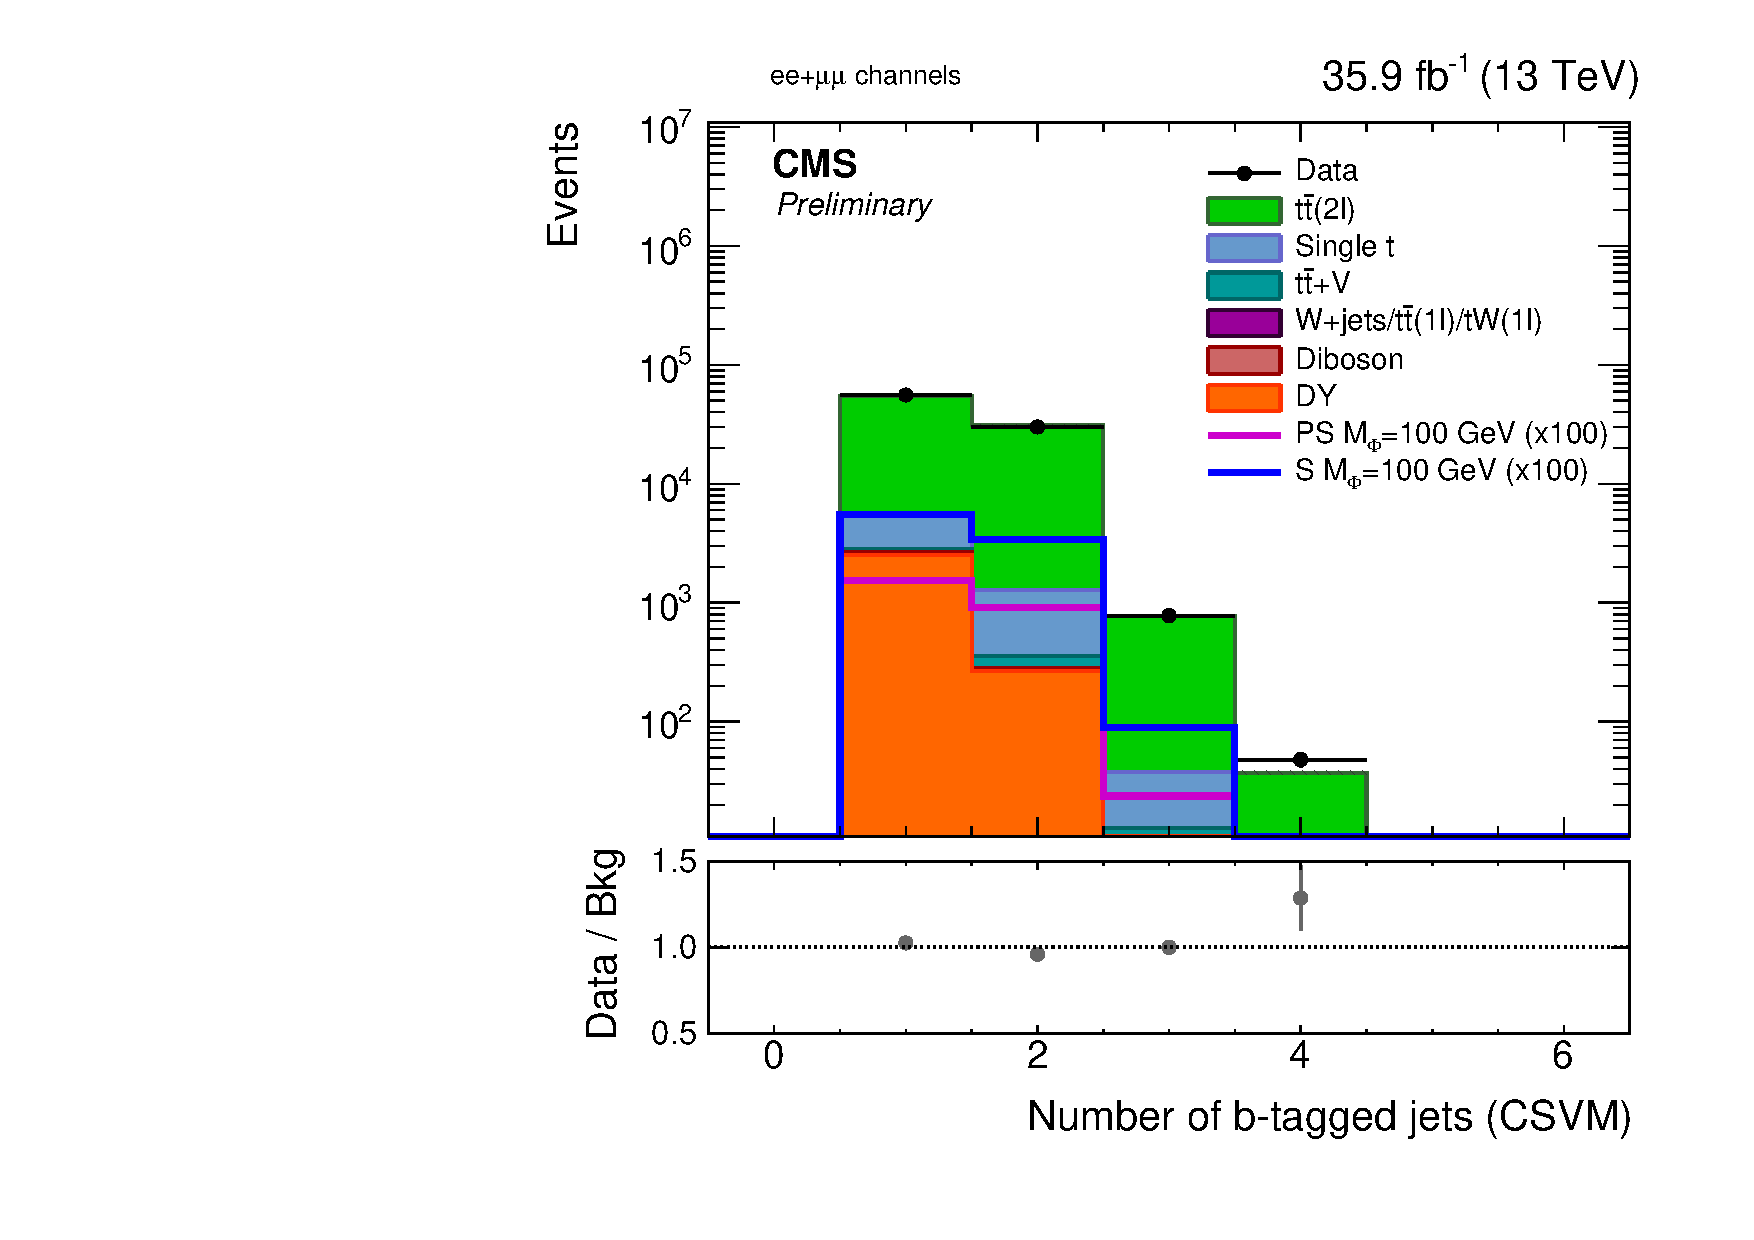
\includegraphics[width=0.4\textwidth]{figs/inclusiveSR/nbjetsm_sf.pdf}} \\
  \subfloat[leading lepton $\pt$]  {\label{subfig:leppt_sf}    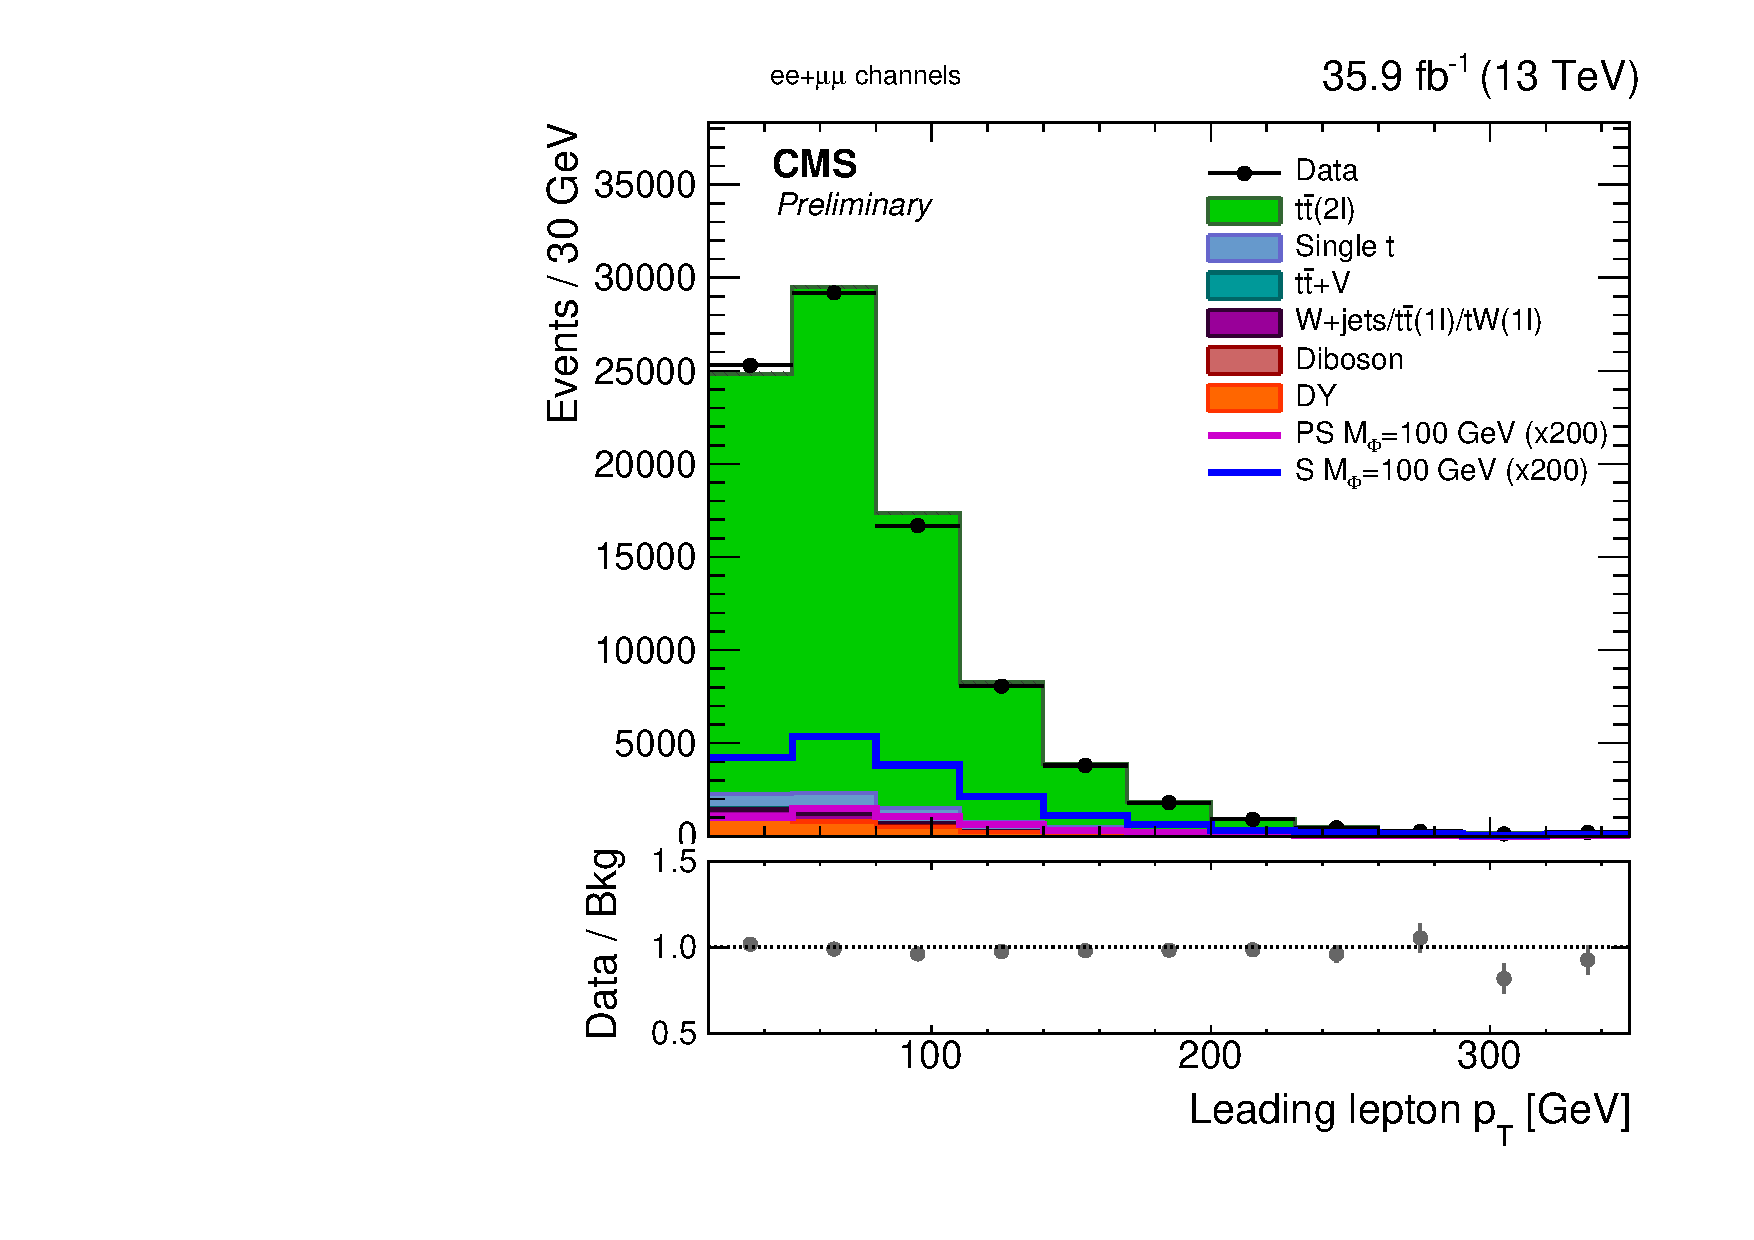
\includegraphics[width=0.4\textwidth]{figs/inclusiveSR/lep1pt_sf.pdf}}
  \subfloat[leading lepton $\eta$] {\label{subfig:lepeta_sf}   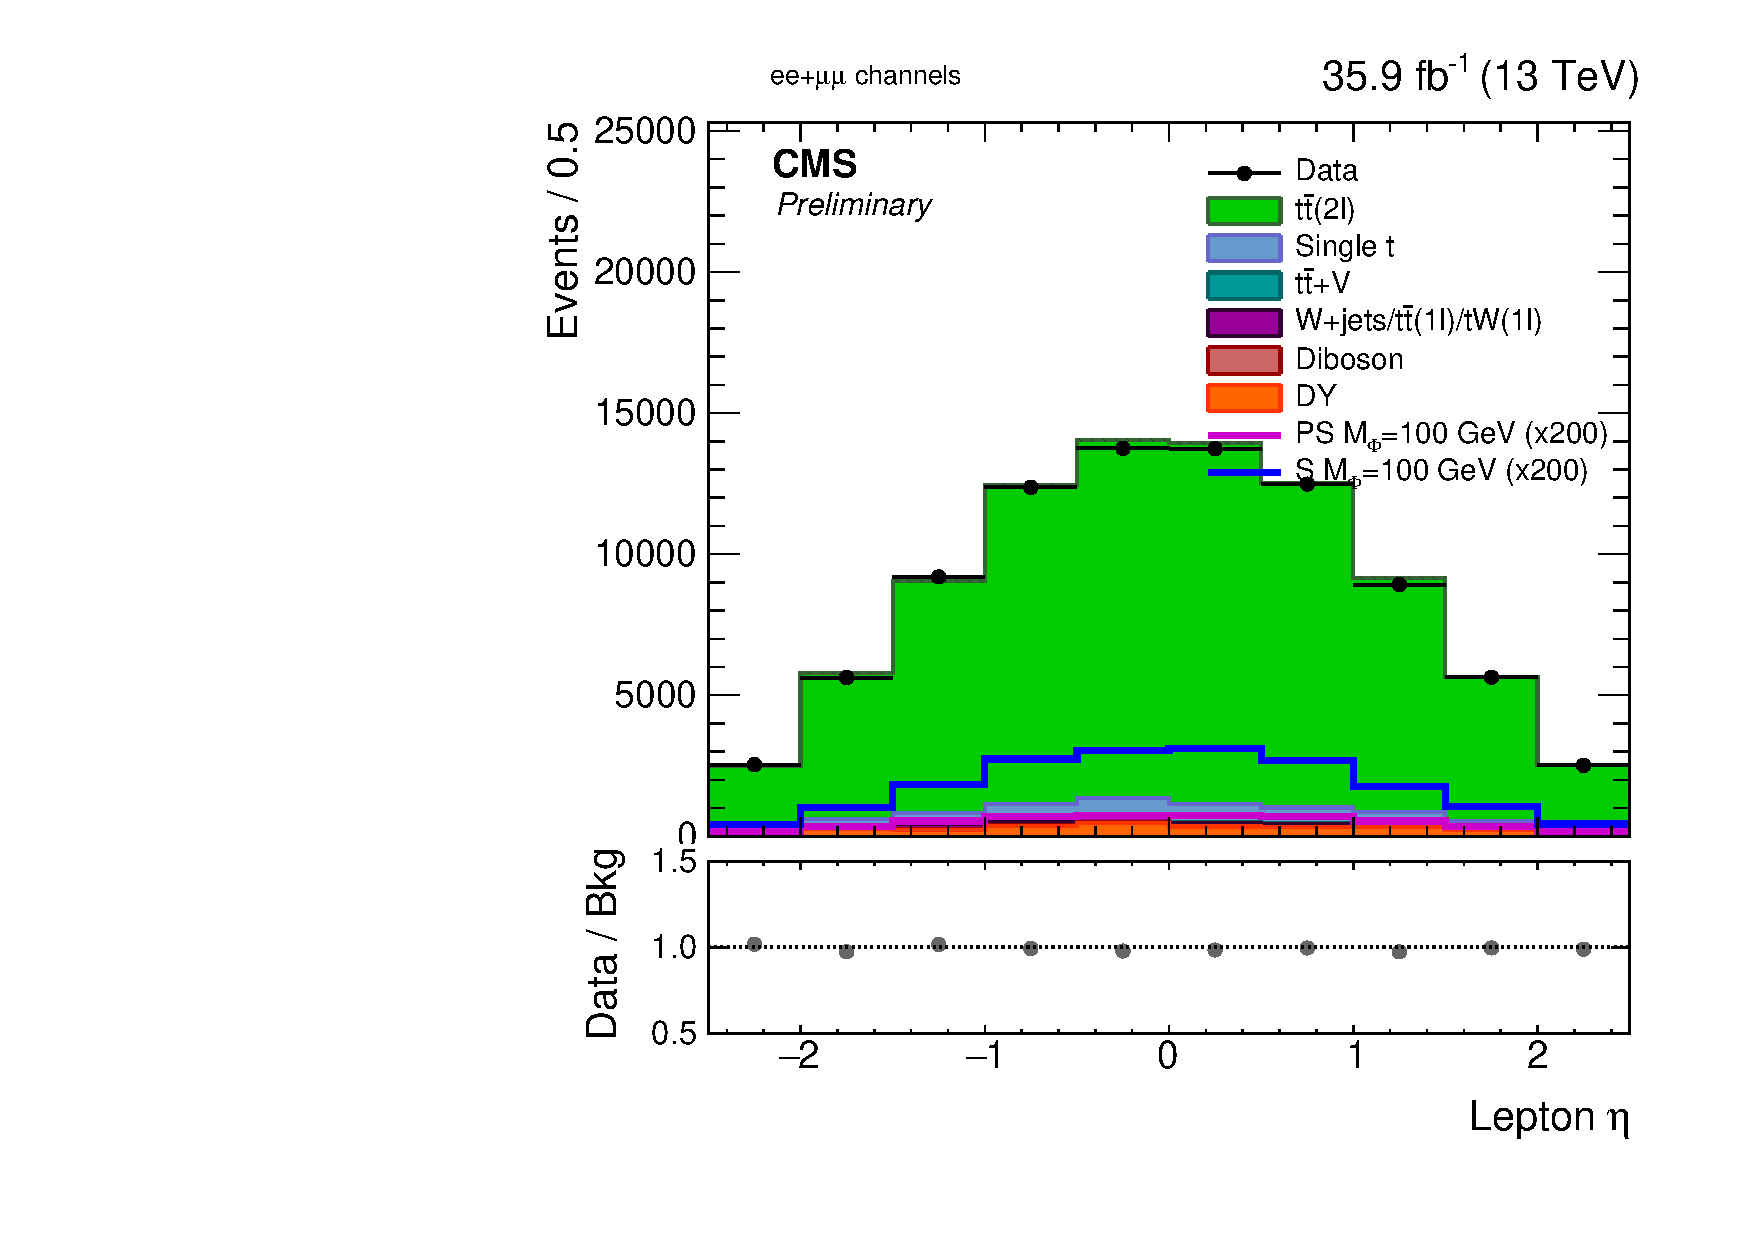
\includegraphics[width=0.4\textwidth]{figs/inclusiveSR/lep1eta_sf.pdf}} \\
  \subfloat[leading jet $\pt$]     {\label{subfig:jetpt_sf}    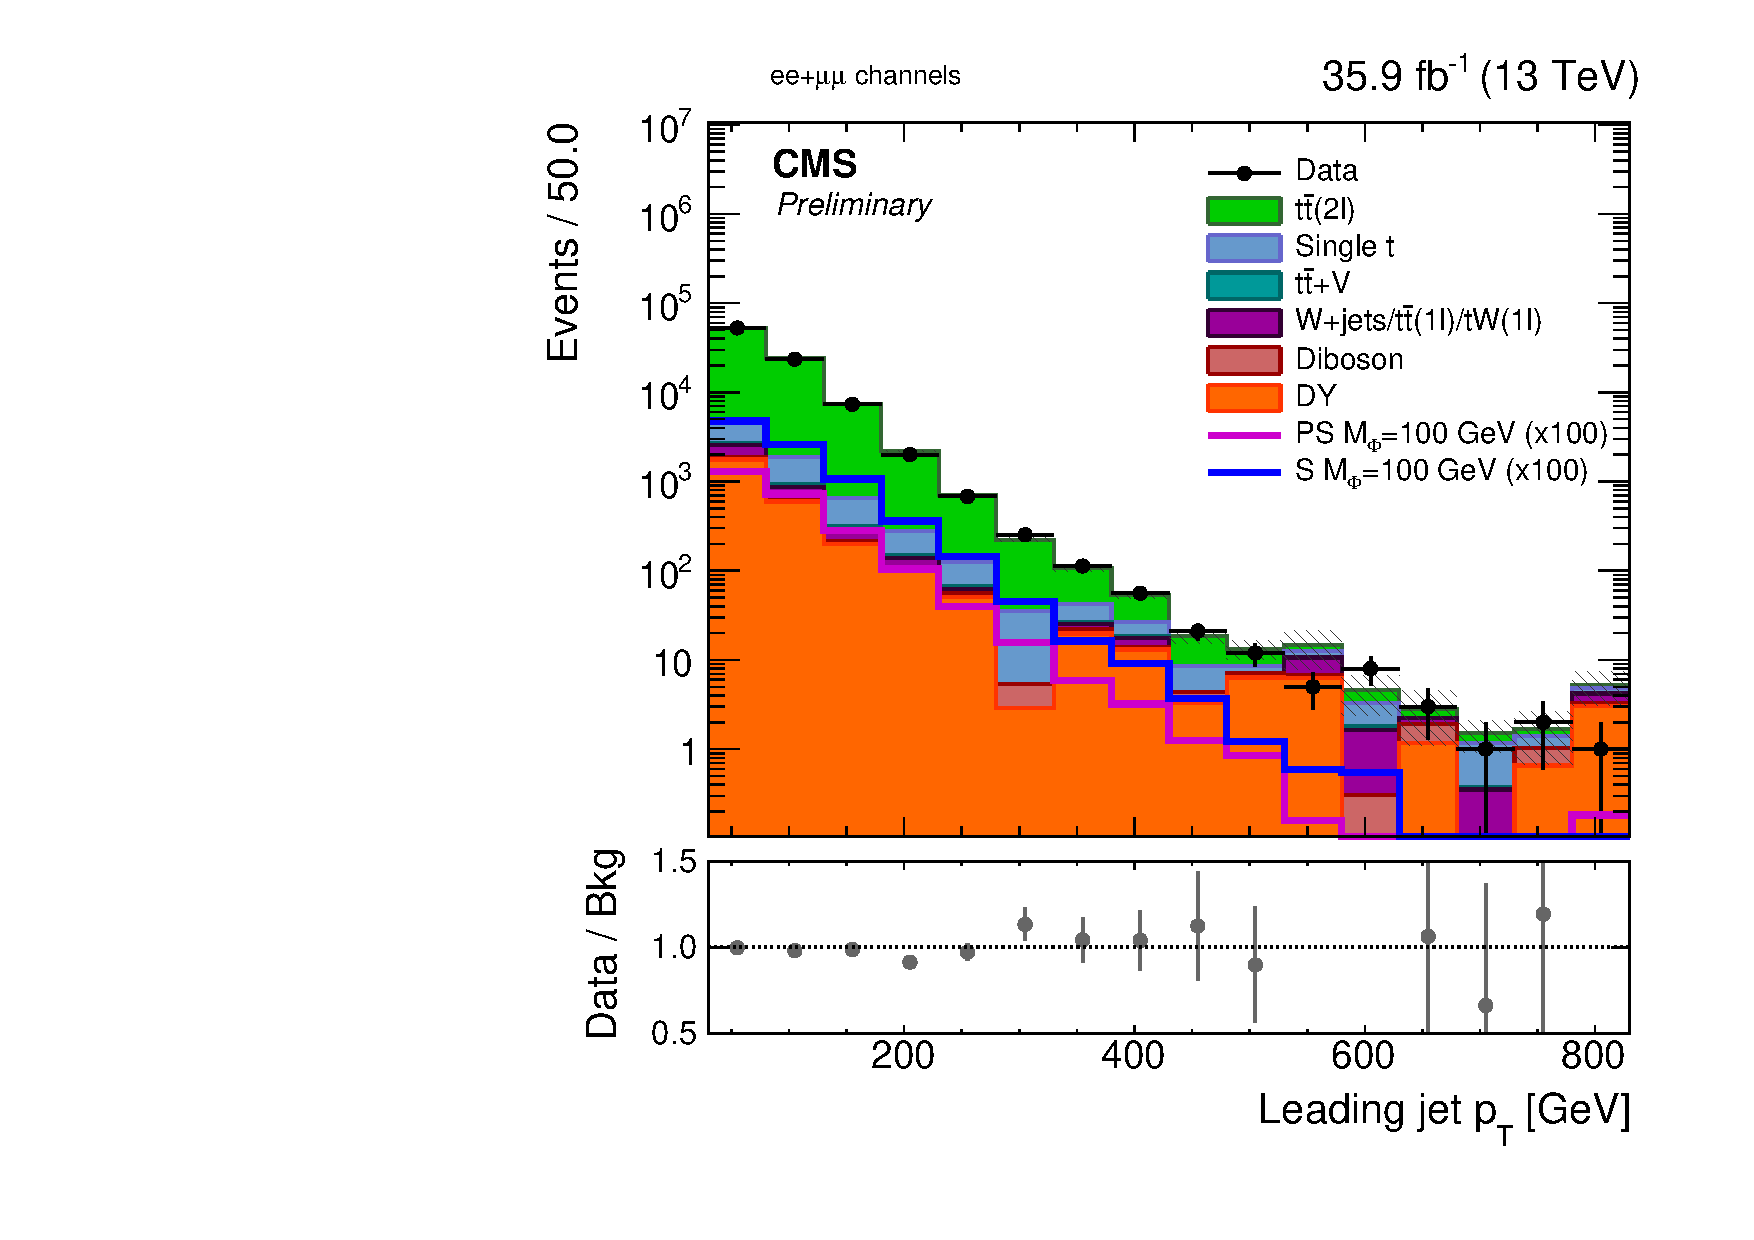
\includegraphics[width=0.4\textwidth]{figs/inclusiveSR/jet1ptlog_sf.pdf}}
  \subfloat[leading jet $\eta$]    {\label{subfig:jeteta_sf}   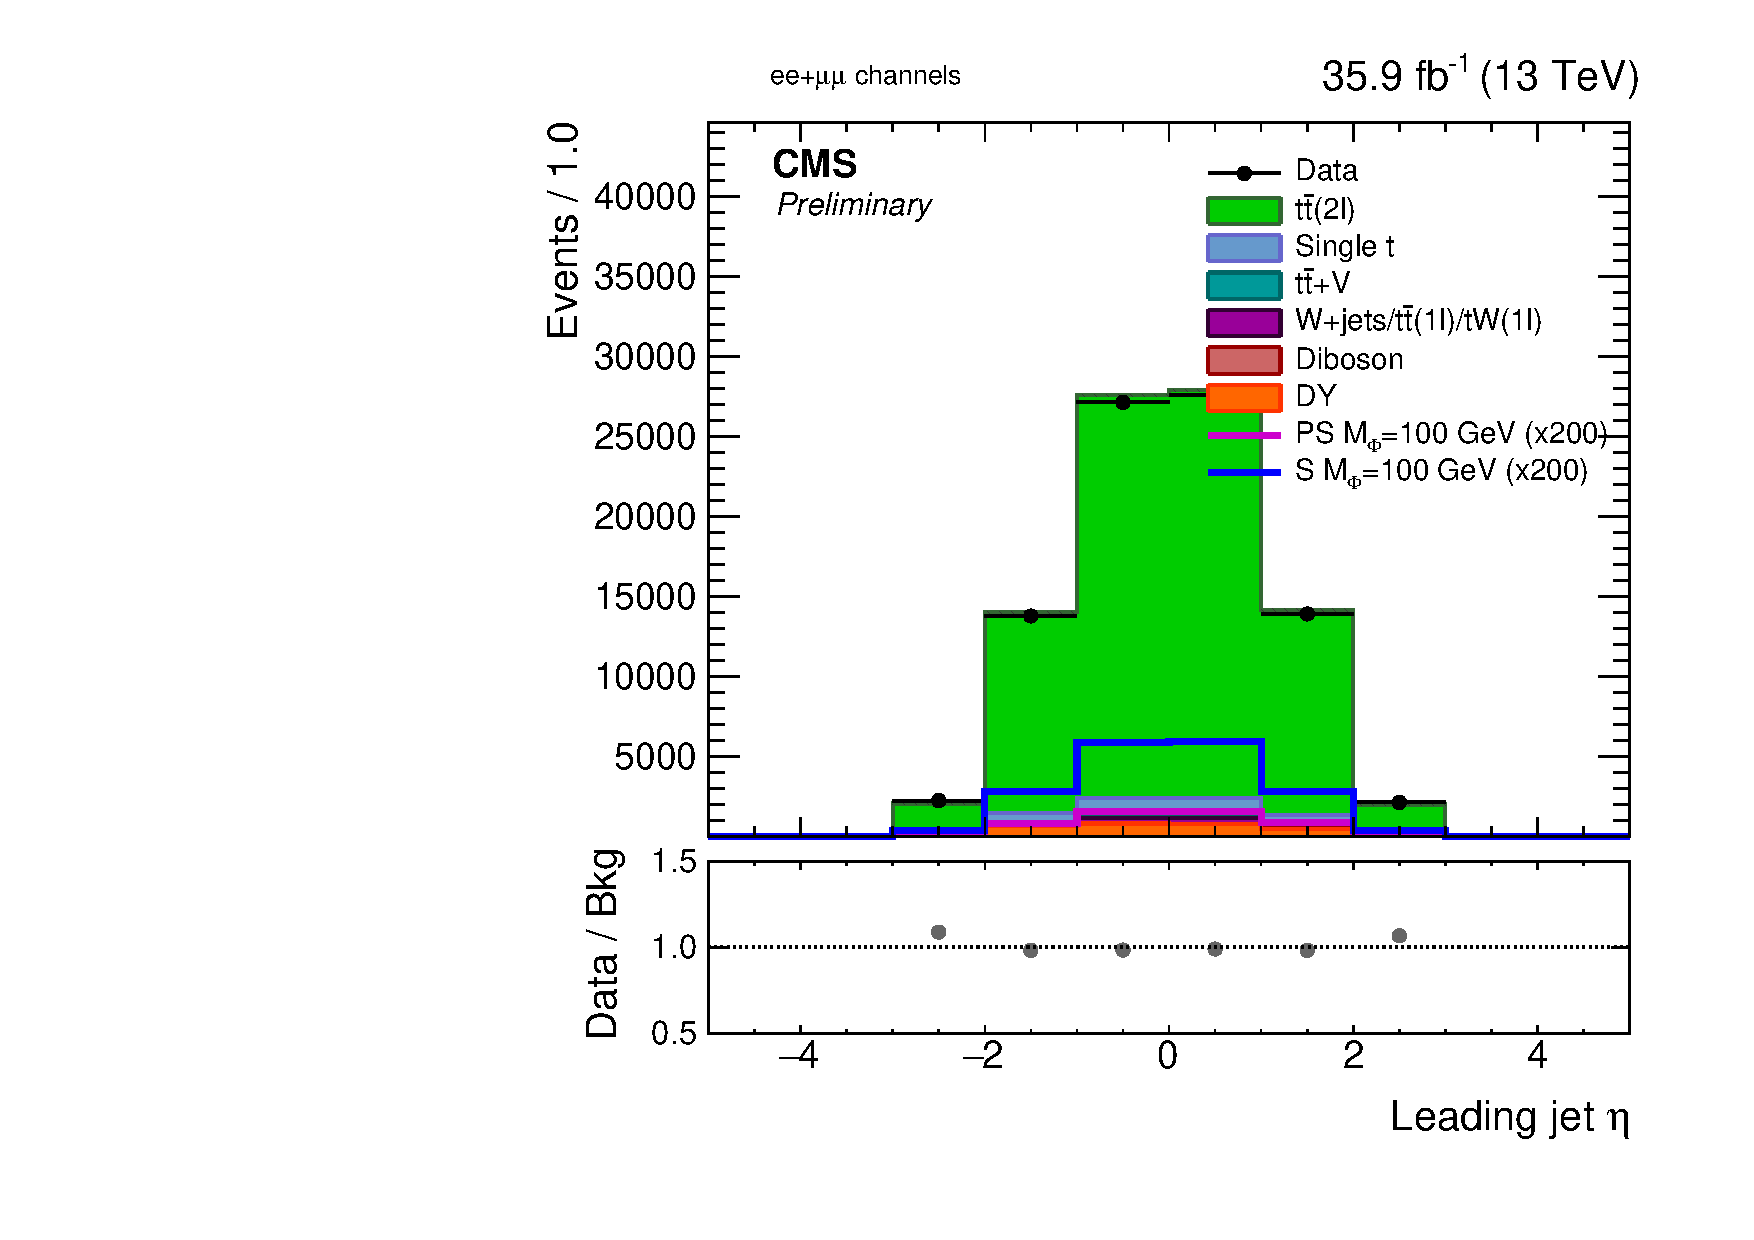
\includegraphics[width=0.4\textwidth]{figs/inclusiveSR/jet1eta_sf.pdf}}
  \caption{Kinematic distributions in the same flavor ($ee+\mu\mu$) channel. Signals with a pseudoscalar (magenta) and scalar (blue) mediator with $\mMed=100\:\GeV$ and $\mDM=1\:\GeV$ are overlayed and scaled by a factor of 200 to illustrate the potential shape differences between the signal and background in the various distributions. The uncertainties shown in these plots on the data and background are purely statistical.}
  \label{fig:dilep_sr_sf}
\end{figure}

\begin{figure}
  \centering
  \subfloat[$\pt^{\ell\ell}$]                  {\label{subfig:dileppt_sf}  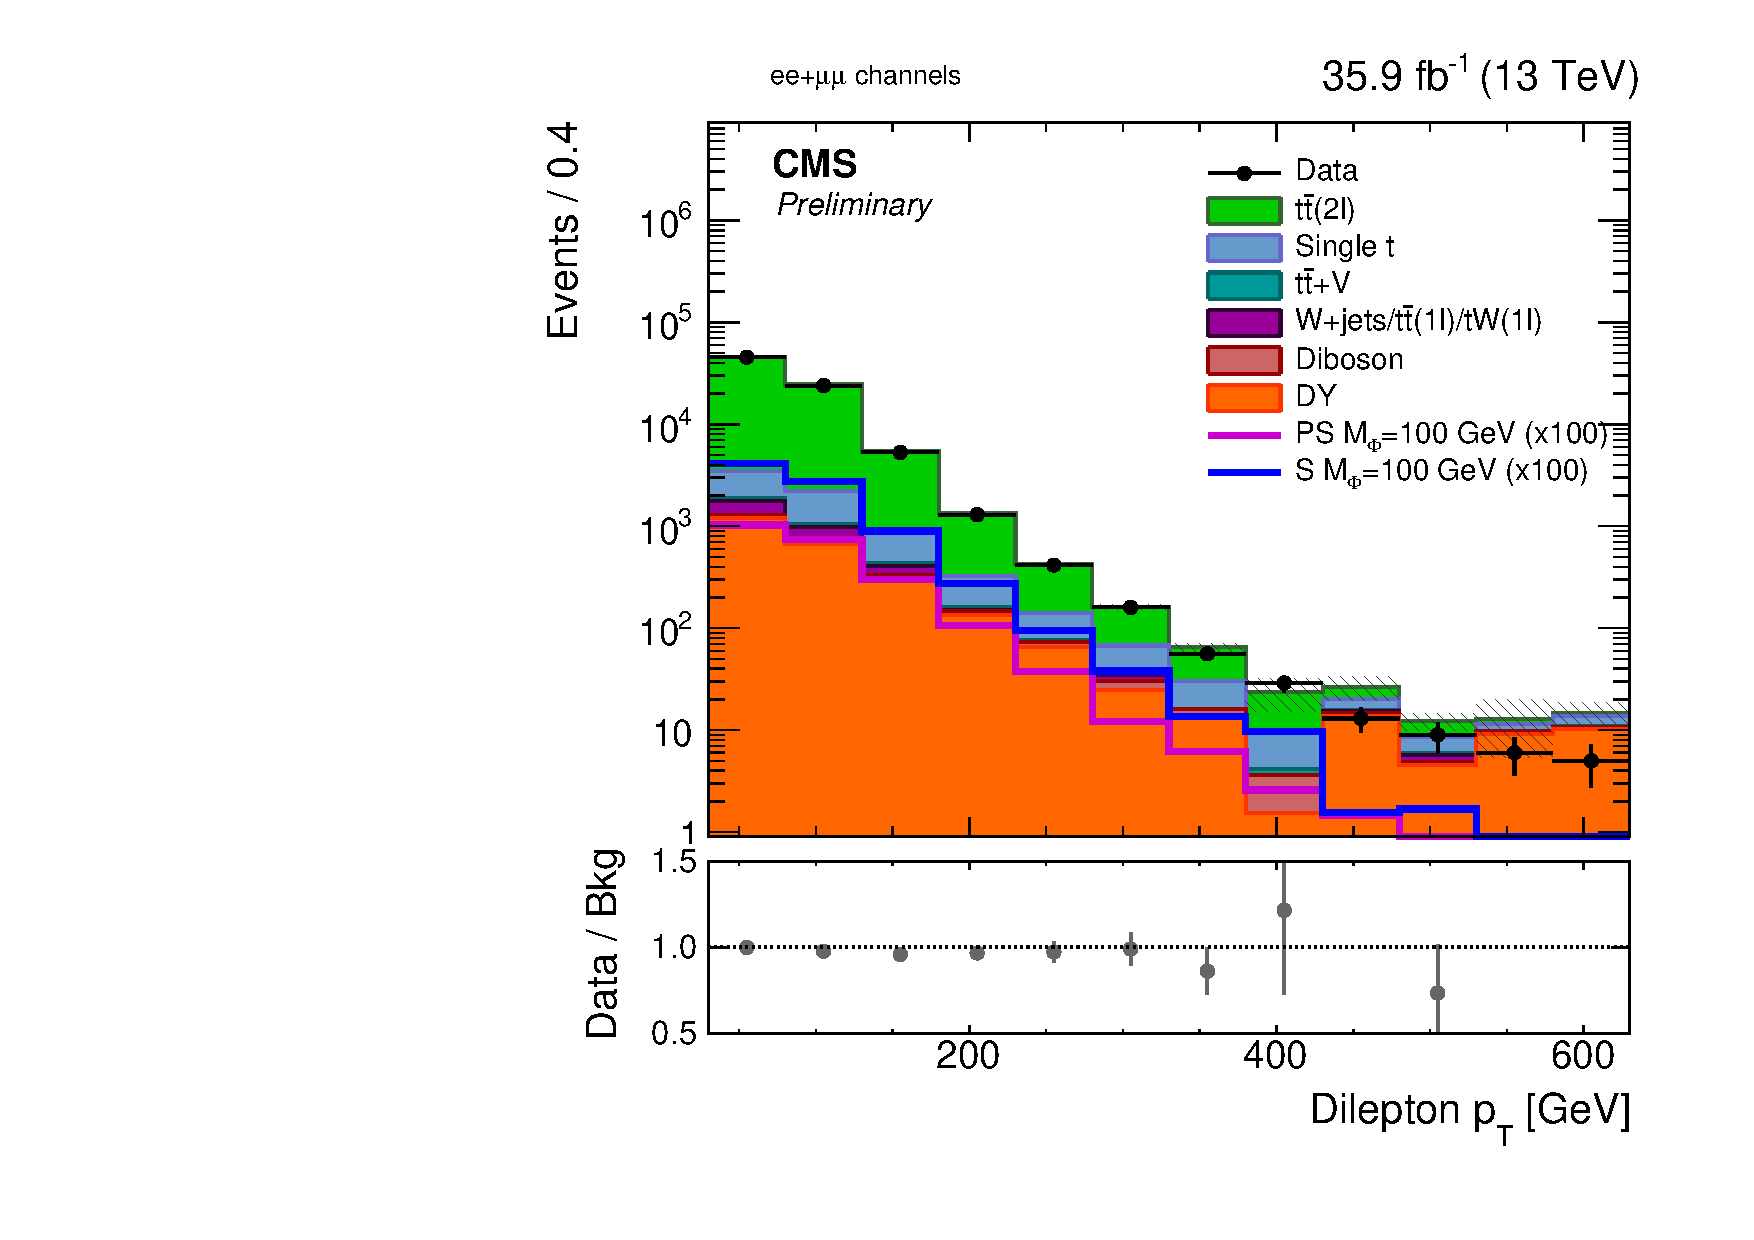
\includegraphics[width=0.45\textwidth]{figs/inclusiveSR/dilepptlog_sf.pdf}}
  \subfloat[$m_{\ell\ell}$]                    {\label{subfig:dilepmass_sf}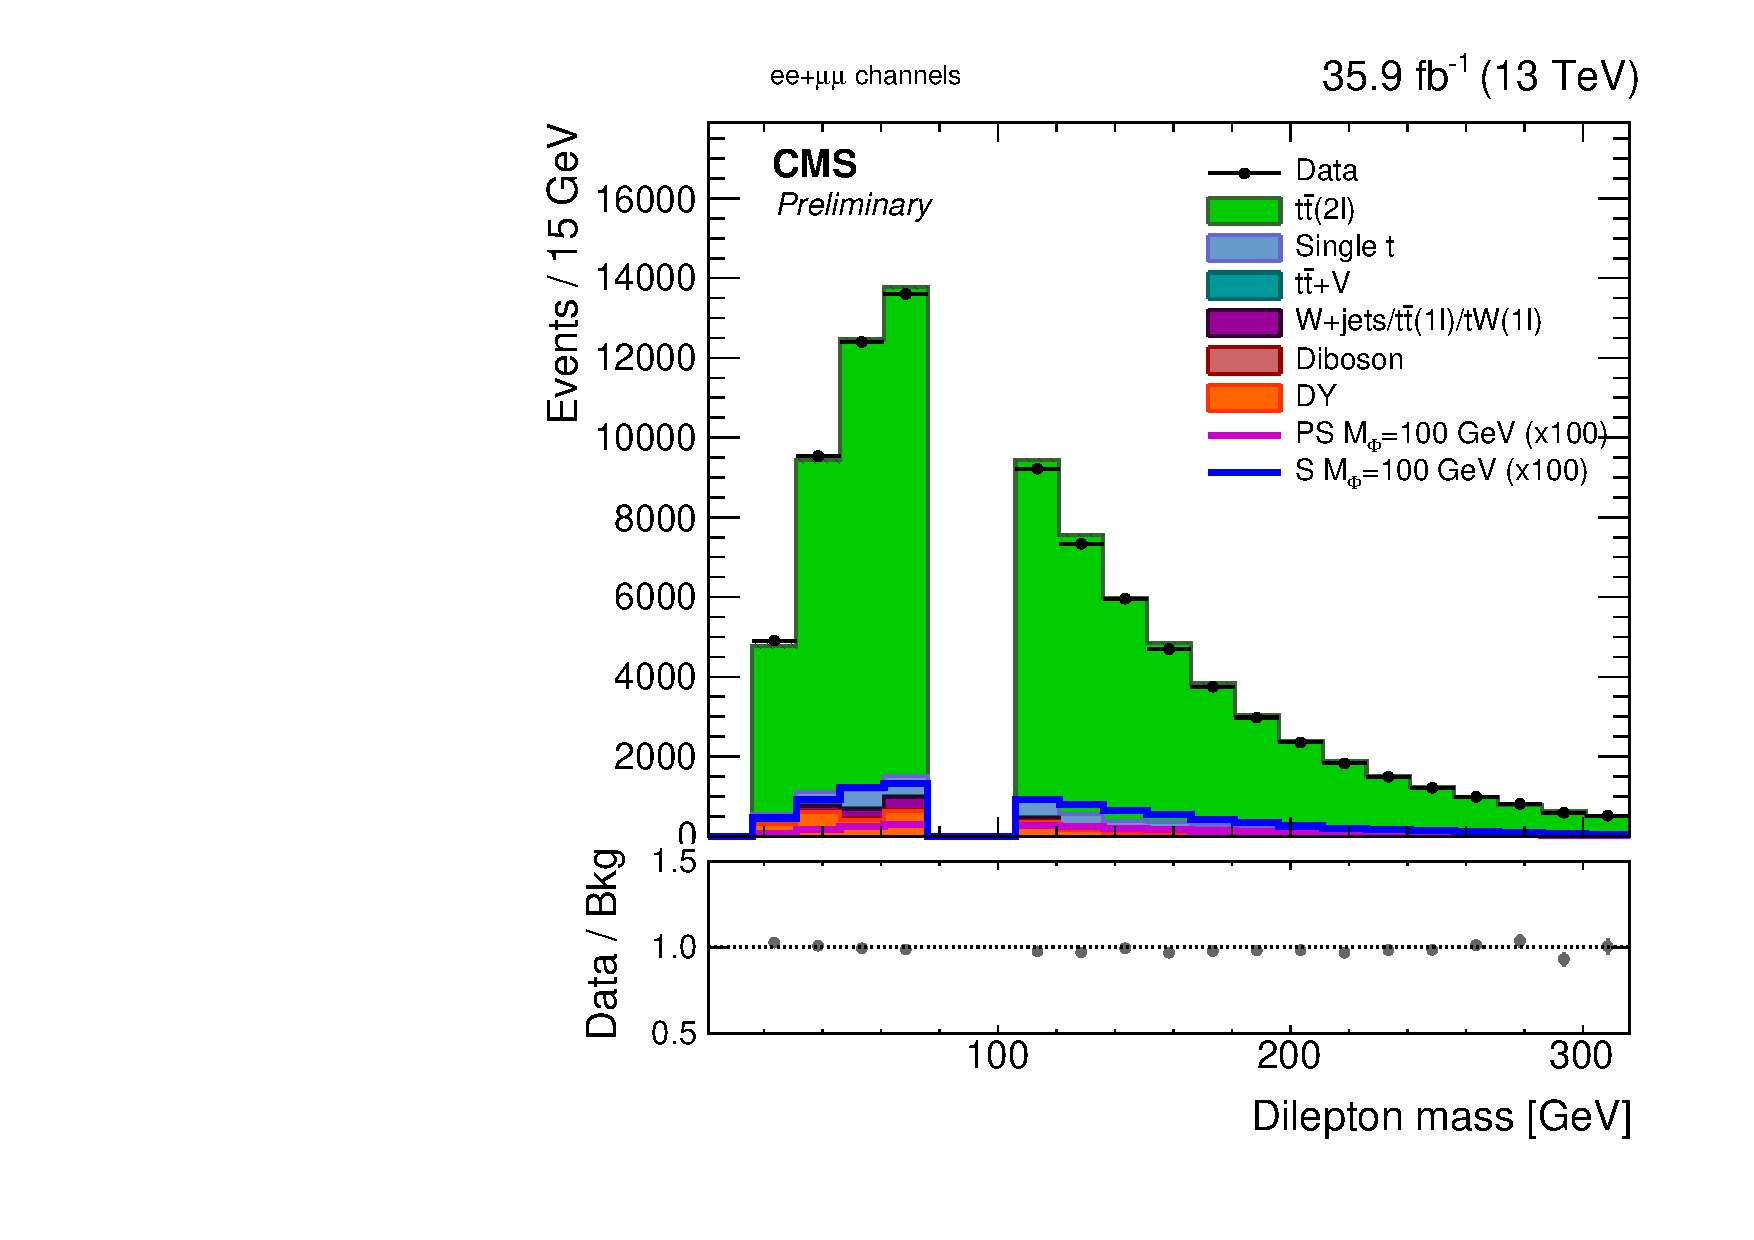
\includegraphics[width=0.45\textwidth]{figs/inclusiveSR/dilepmass_sf.pdf}} \\
%  \subfloat[$\Delta\phi(\vec{p}_{\text{T}}^{\ell\ell},\ptvecmiss)$] {\label{subfig:dphidilepmet_sf}  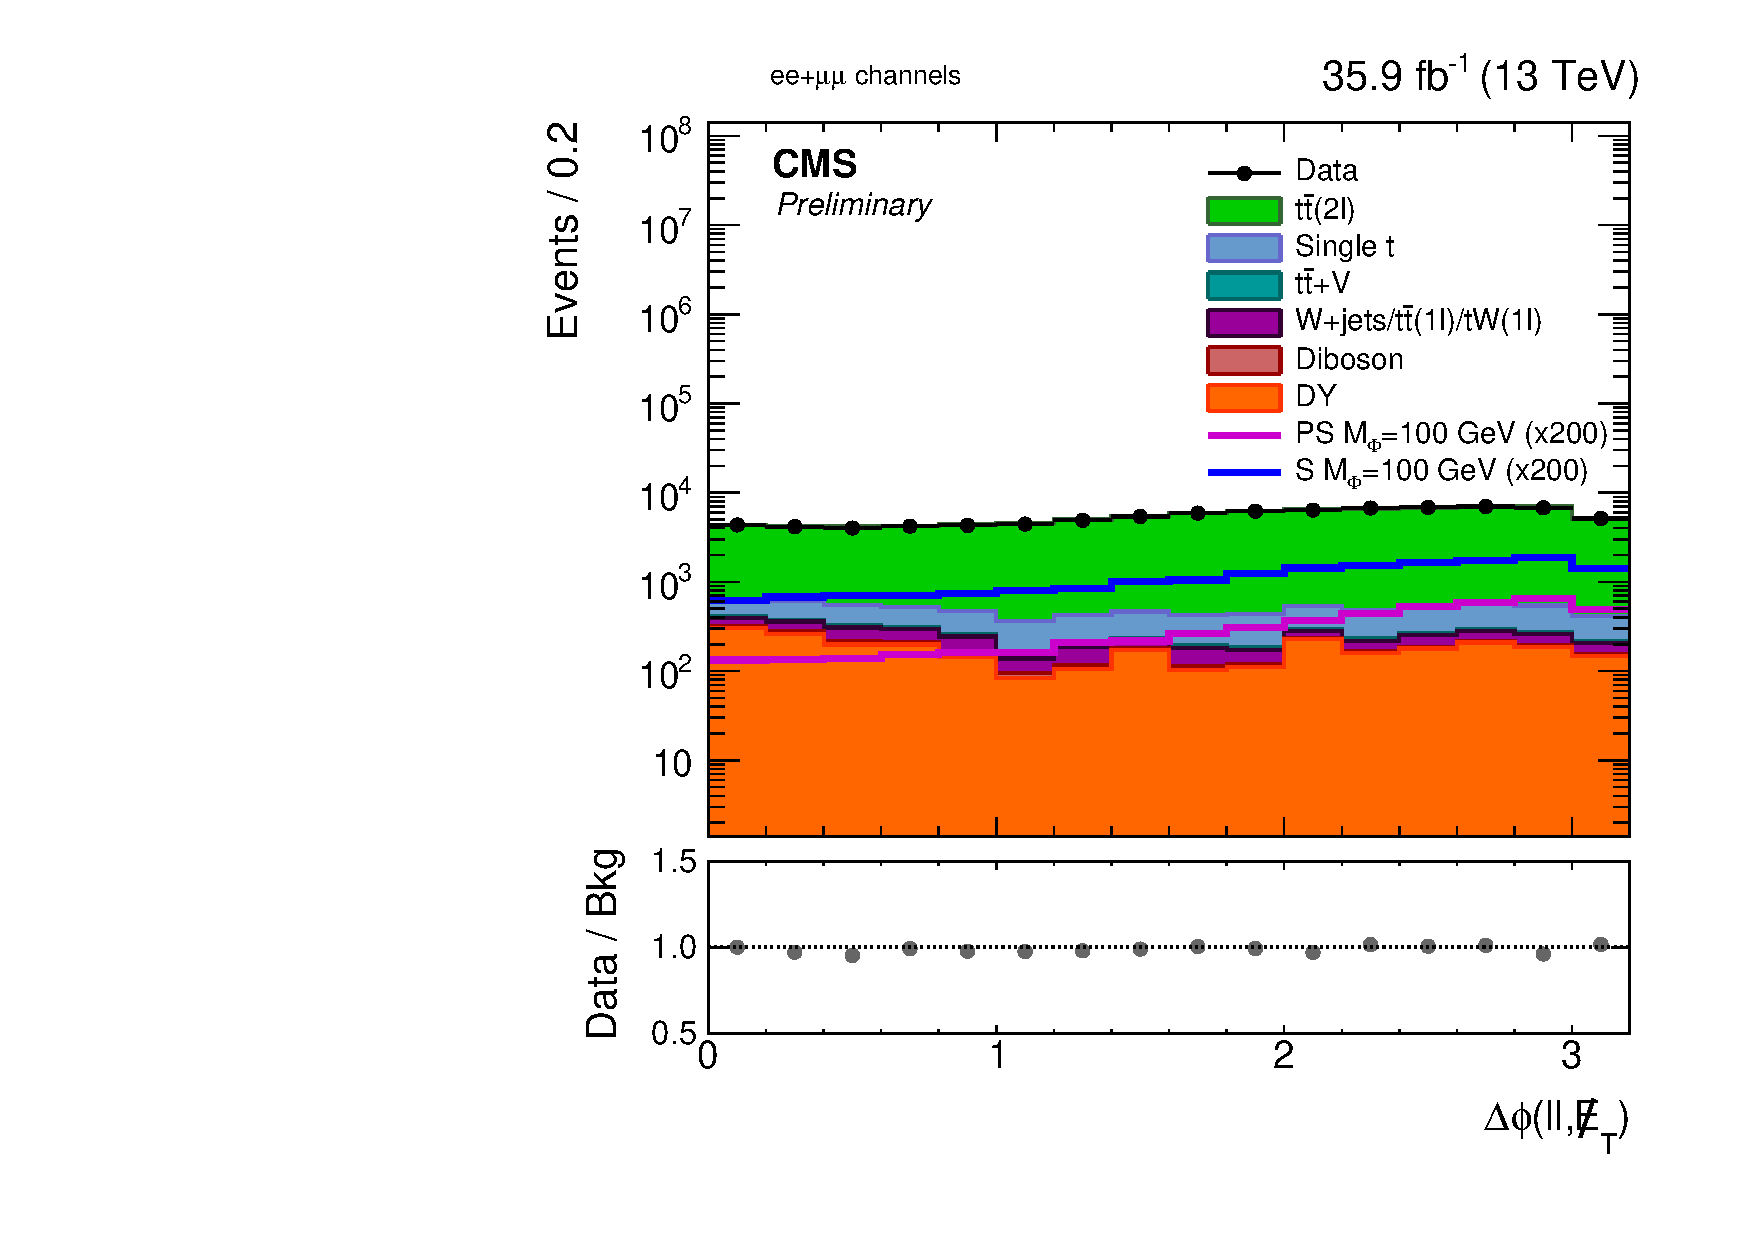
\includegraphics[width=0.4\textwidth]{figs/inclusiveSR/dphidilepmetlog_sf.pdf}}
  \subfloat[\ptmiss]                           {\label{subfig:met_sf}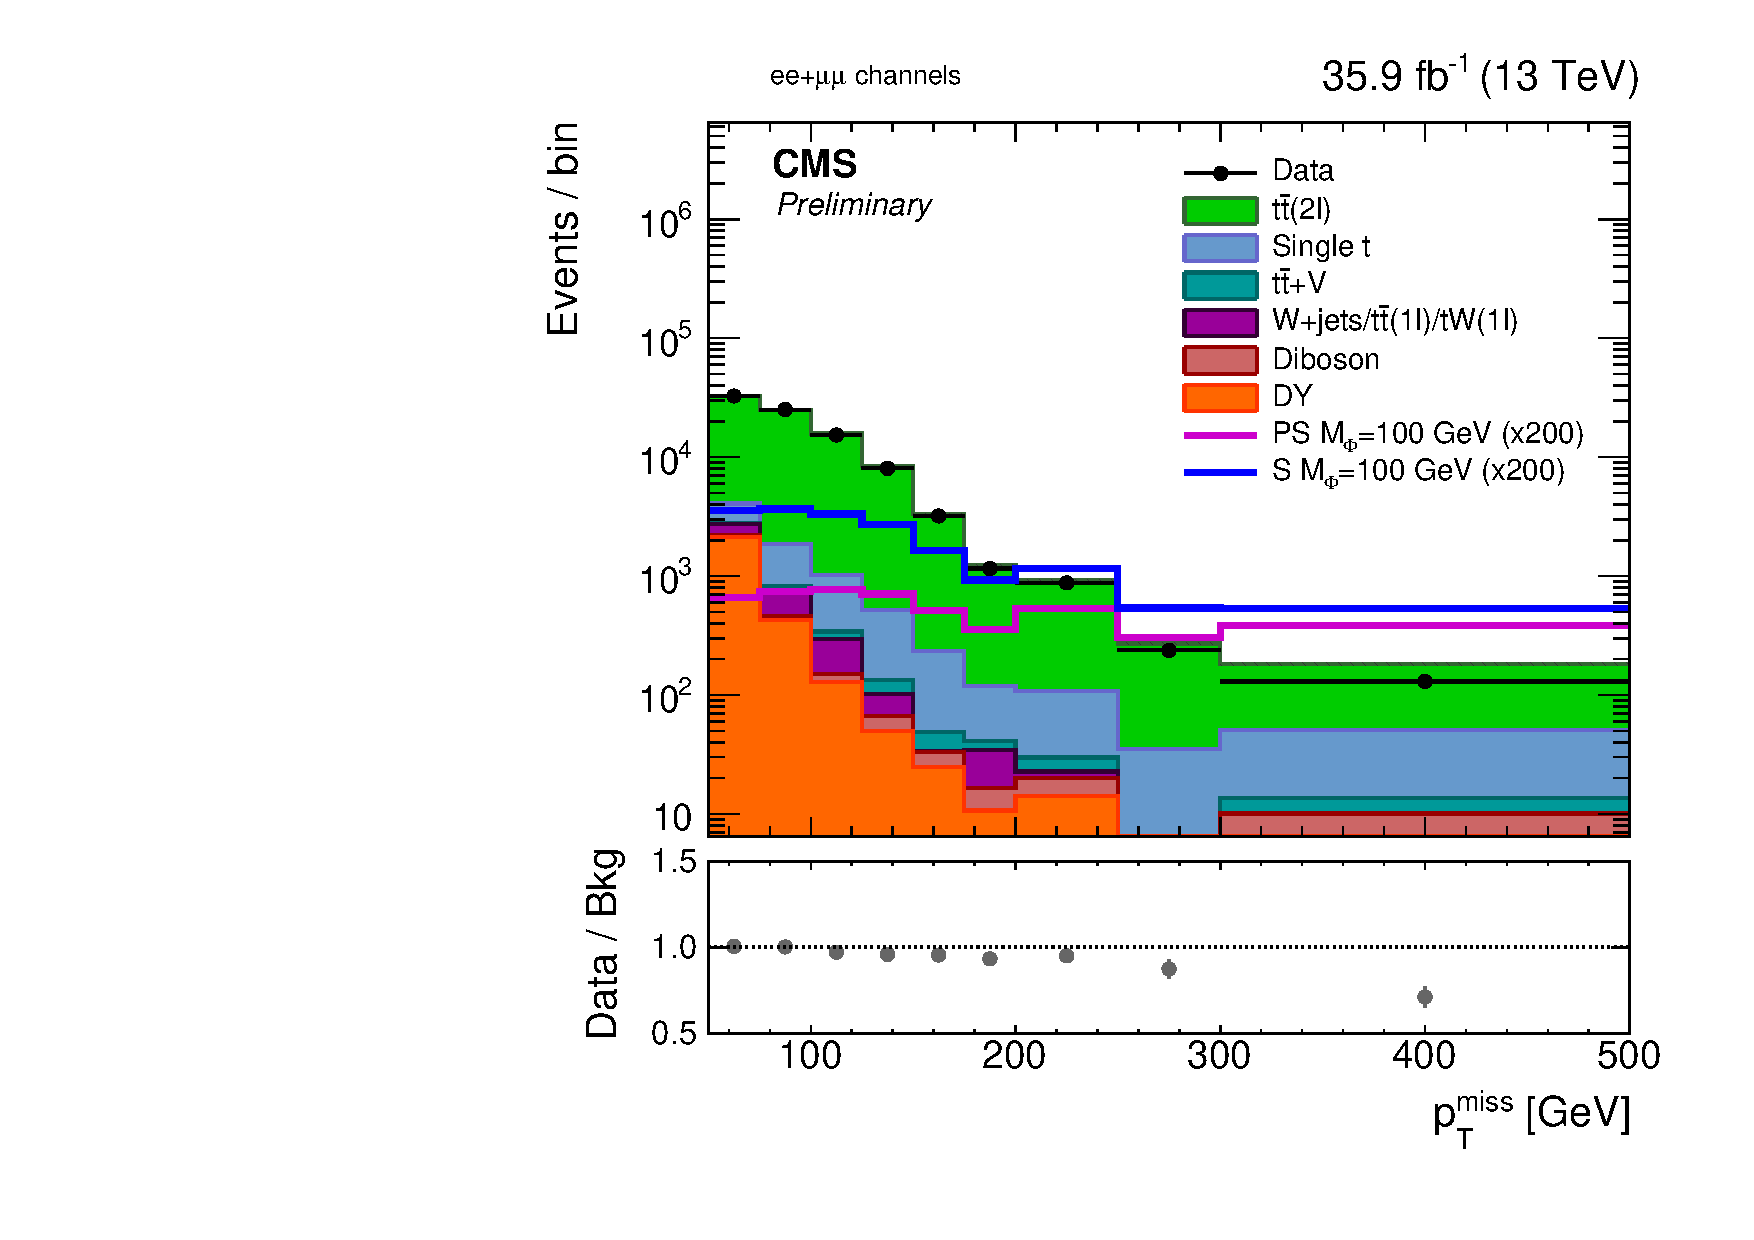
\includegraphics[width=0.45\textwidth]{figs/inclusiveSR/metlog_sf.pdf}}
  \caption{Kinematic distributions in the same flavor ($ee+\mu\mu$) channel. Signals with a pseudoscalar (magenta) and scalar (blue) mediator with $\mMed=100\:\GeV$ and $\mDM=1\:\GeV$ are overlayed and scaled by a factor of 200 to illustrate the potential shape differences between the signal and background in the various distributions. The uncertainties shown in these plots on the data and background are purely statistical.}
  \label{fig:dilep_sr_sf}
\end{figure}

\begin{figure}
  \centering
  \subfloat[$N_{\textrm{jets}}$]   {\label{subfig:njets_em}    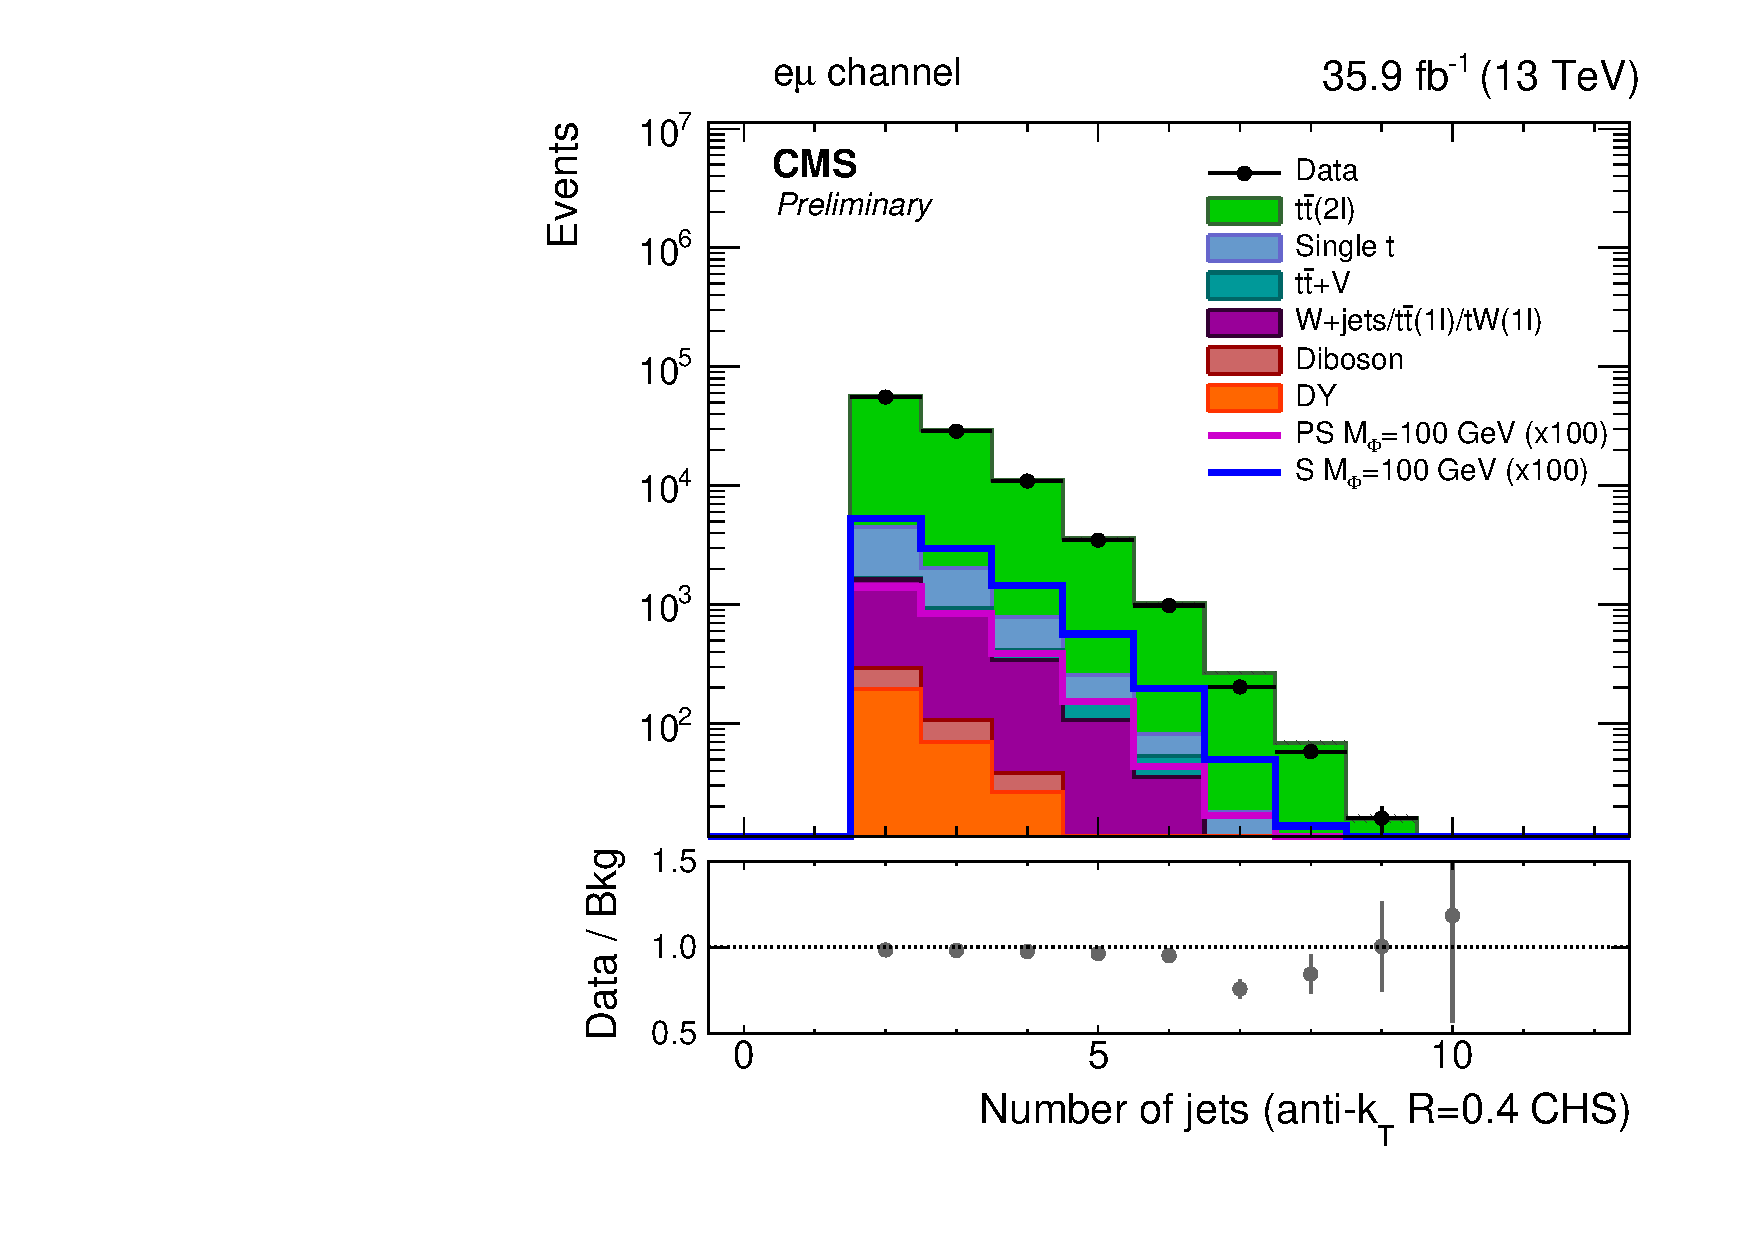
\includegraphics[width=0.4\textwidth]{figs/inclusiveSR/njets_em.pdf}}
  \subfloat[$N_{\textrm{b-jets}}$] {\label{subfig:nbjets_em}   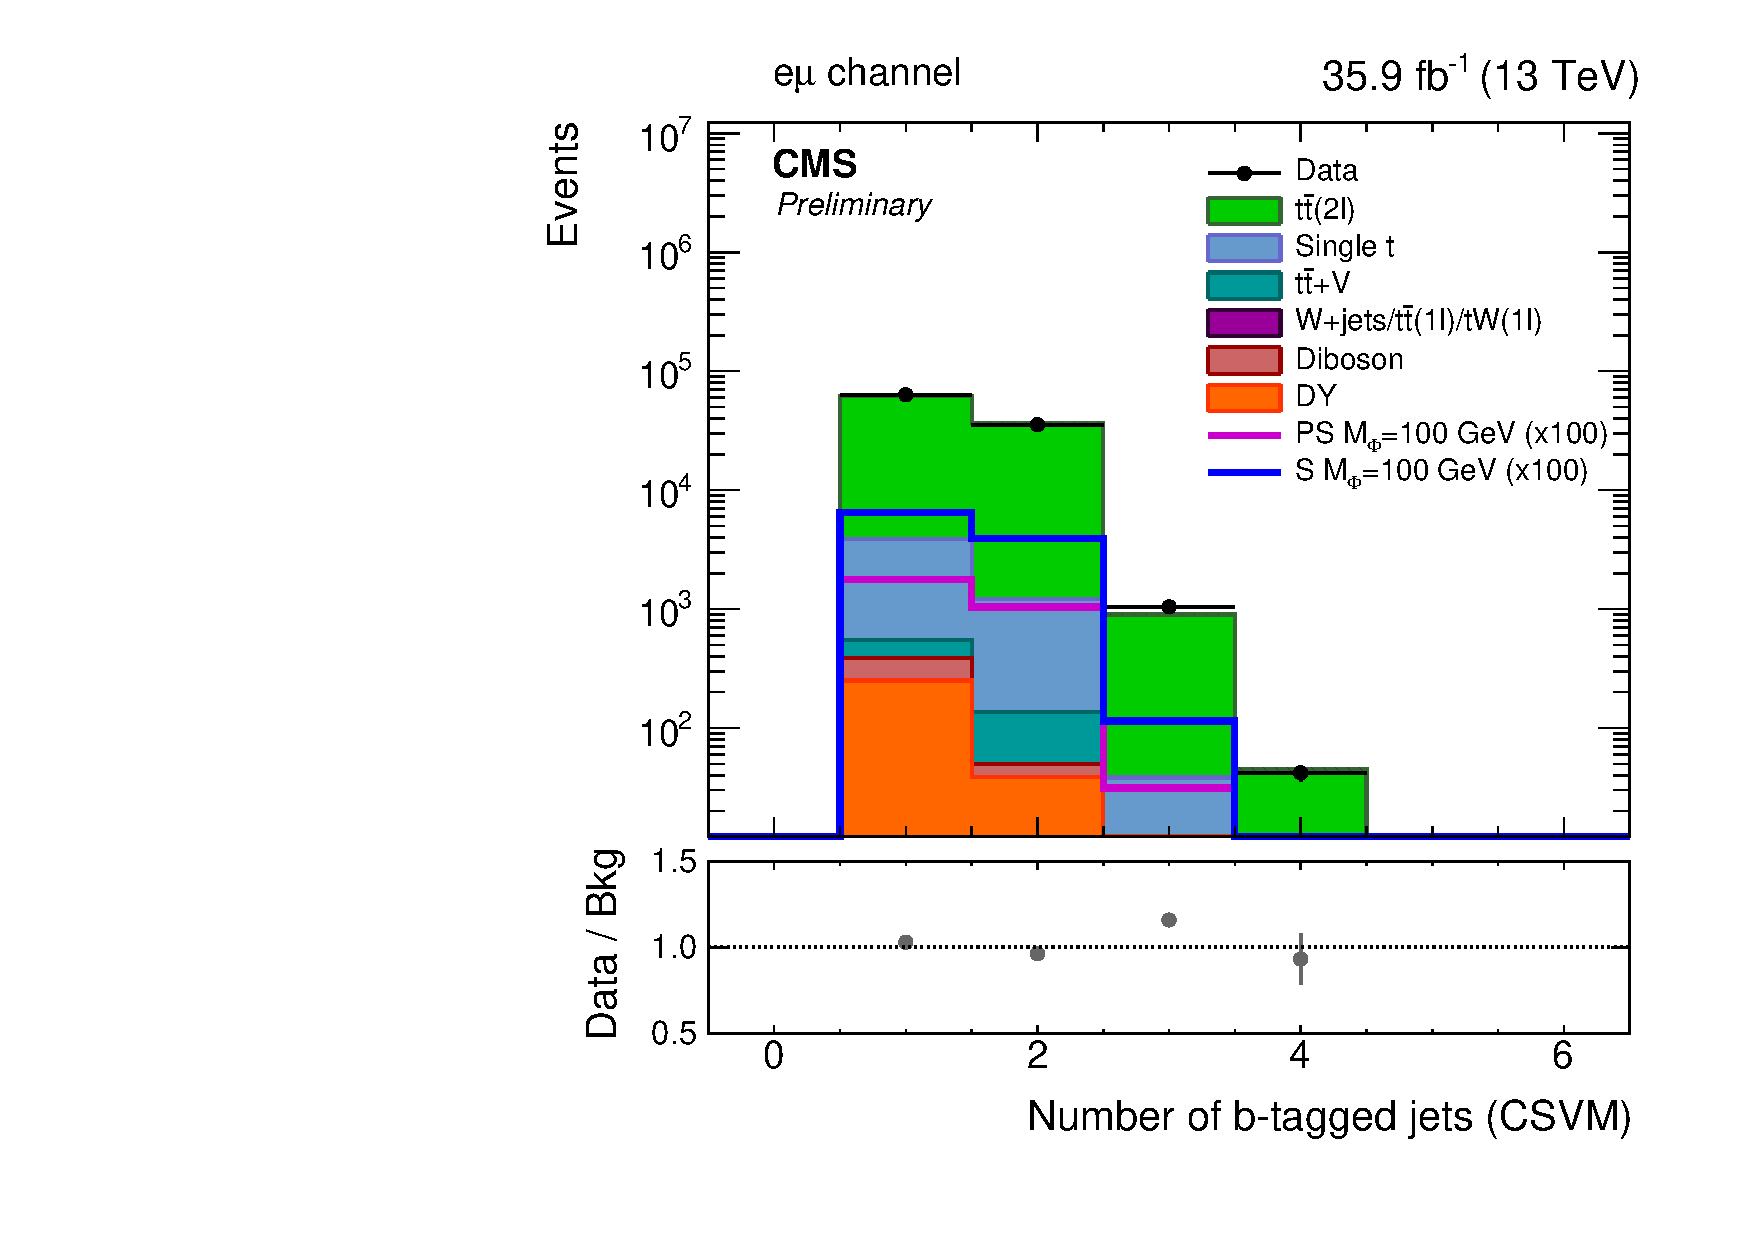
\includegraphics[width=0.4\textwidth]{figs/inclusiveSR/nbjetsm_em.pdf}} \\
  \subfloat[leading lepton $\pt$]  {\label{subfig:leppt_em}    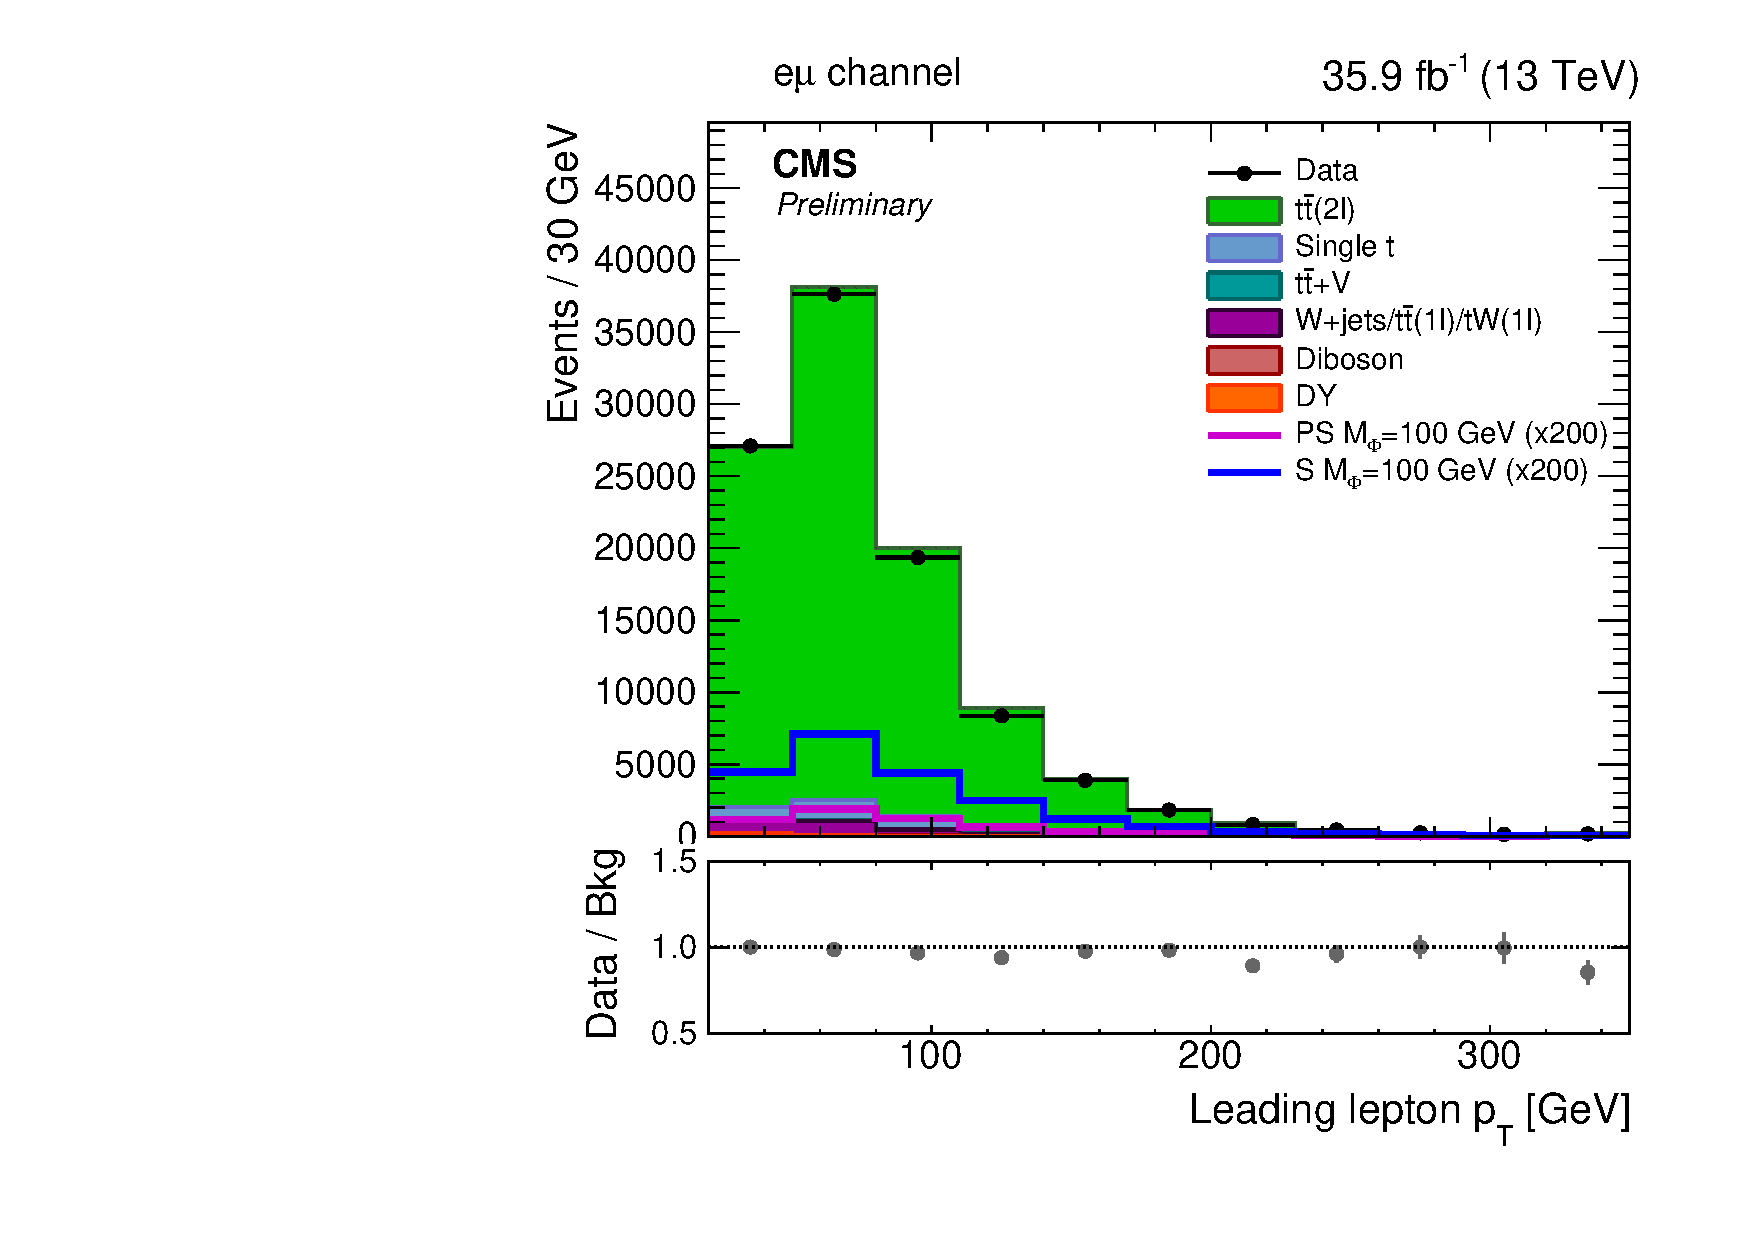
\includegraphics[width=0.4\textwidth]{figs/inclusiveSR/lep1pt_em.pdf}}
  \subfloat[leading lepton $\eta$] {\label{subfig:lepeta_em}   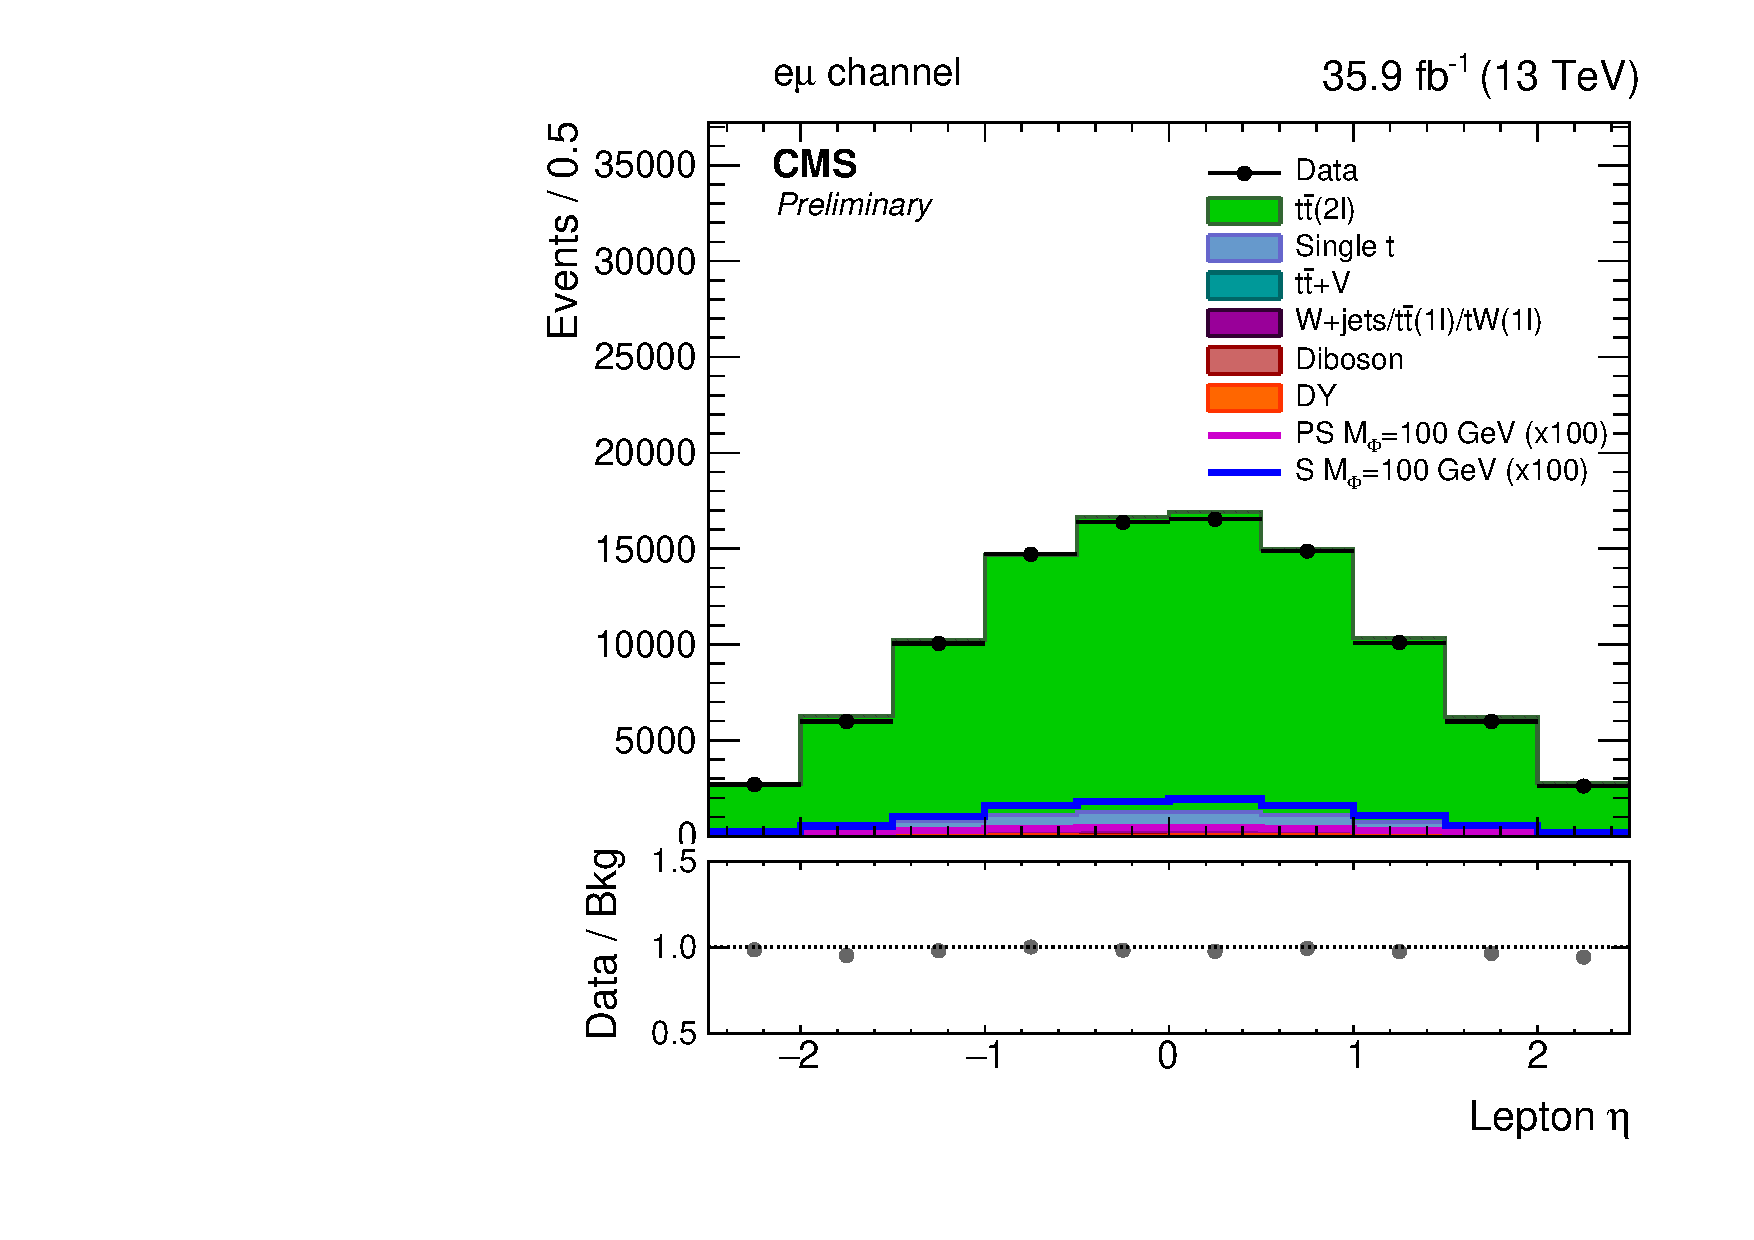
\includegraphics[width=0.4\textwidth]{figs/inclusiveSR/lep1eta_em.pdf}} \\
  \subfloat[leading jet $\pt$]     {\label{subfig:jetpt_em}    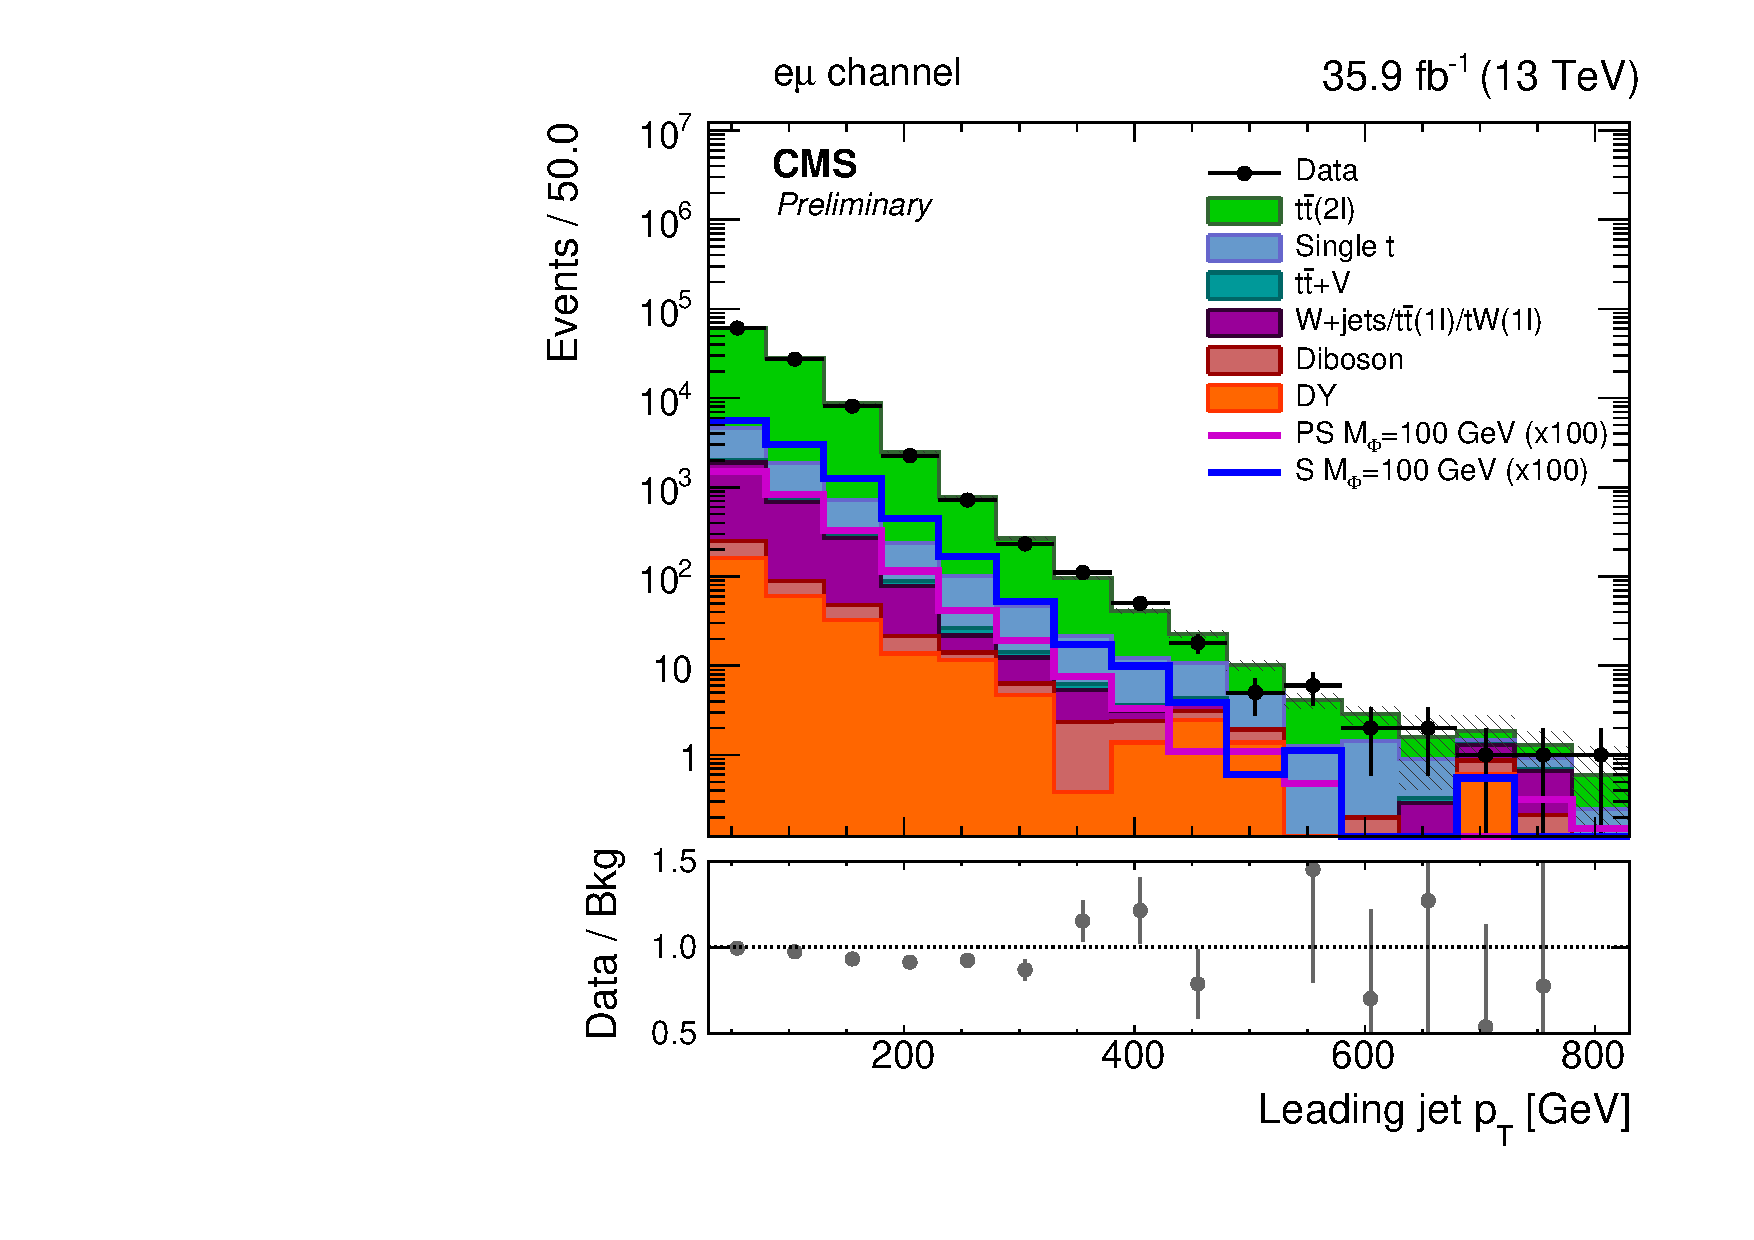
\includegraphics[width=0.4\textwidth]{figs/inclusiveSR/jet1ptlog_em.pdf}}
  \subfloat[leading jet $\eta$]    {\label{subfig:jeteta_em}   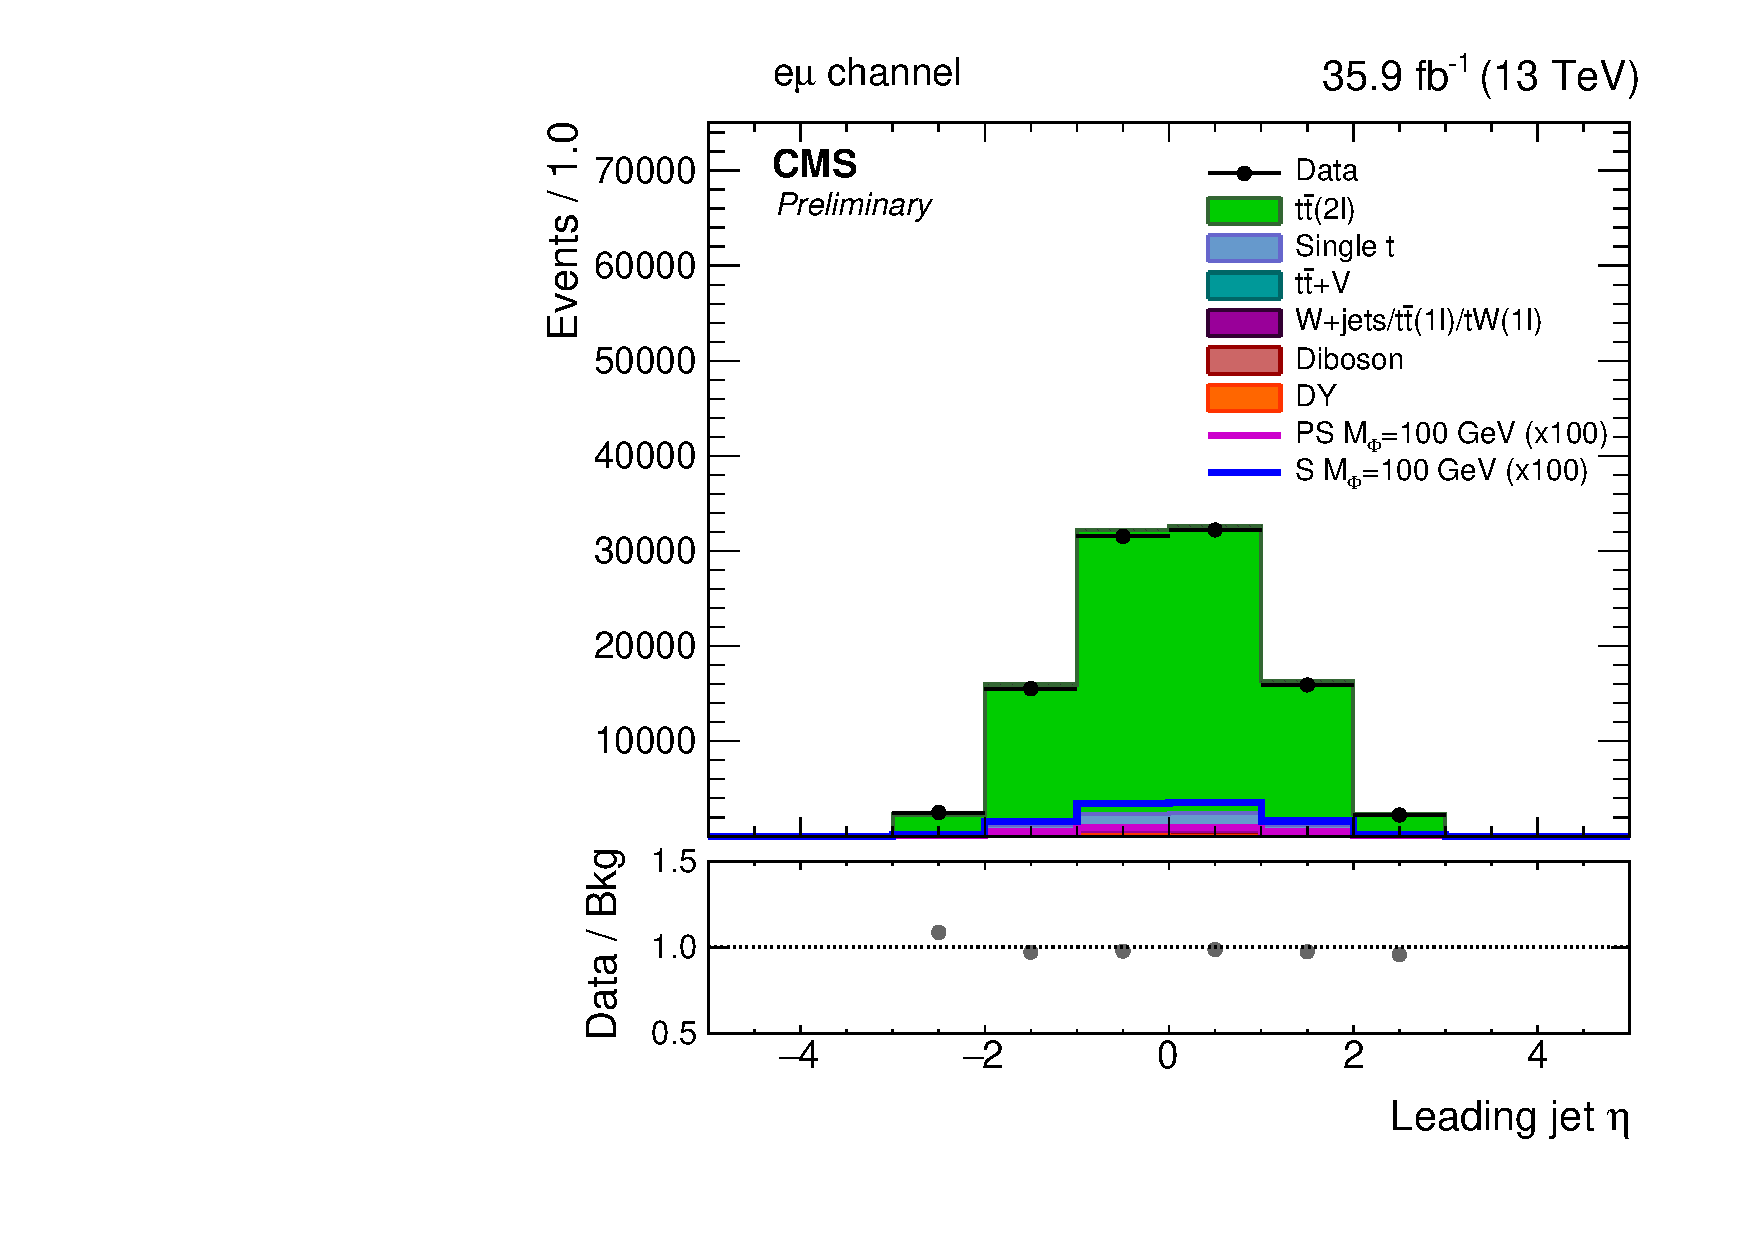
\includegraphics[width=0.4\textwidth]{figs/inclusiveSR/jet1eta_em.pdf}}
  \caption{Kinematic distributions in the same flavor ($e\mu$) channel. Signals with a pseudoscalar (magenta) and scalar (blue) mediator with $\mMed=100\:\GeV$ and $\mDM=1\:\GeV$ are overlayed and scaled by a factor of 200 to illustrate the potential shape differences between the signal and background in the various distributions. The uncertainties shown in these plots on the data and background are purely statistical.}
  \label{fig:dilep_sr_em}
\end{figure}

\begin{figure}
  \centering
  \subfloat[$\pt^{\ell\ell}$]                  {\label{subfig:dileppt_em}  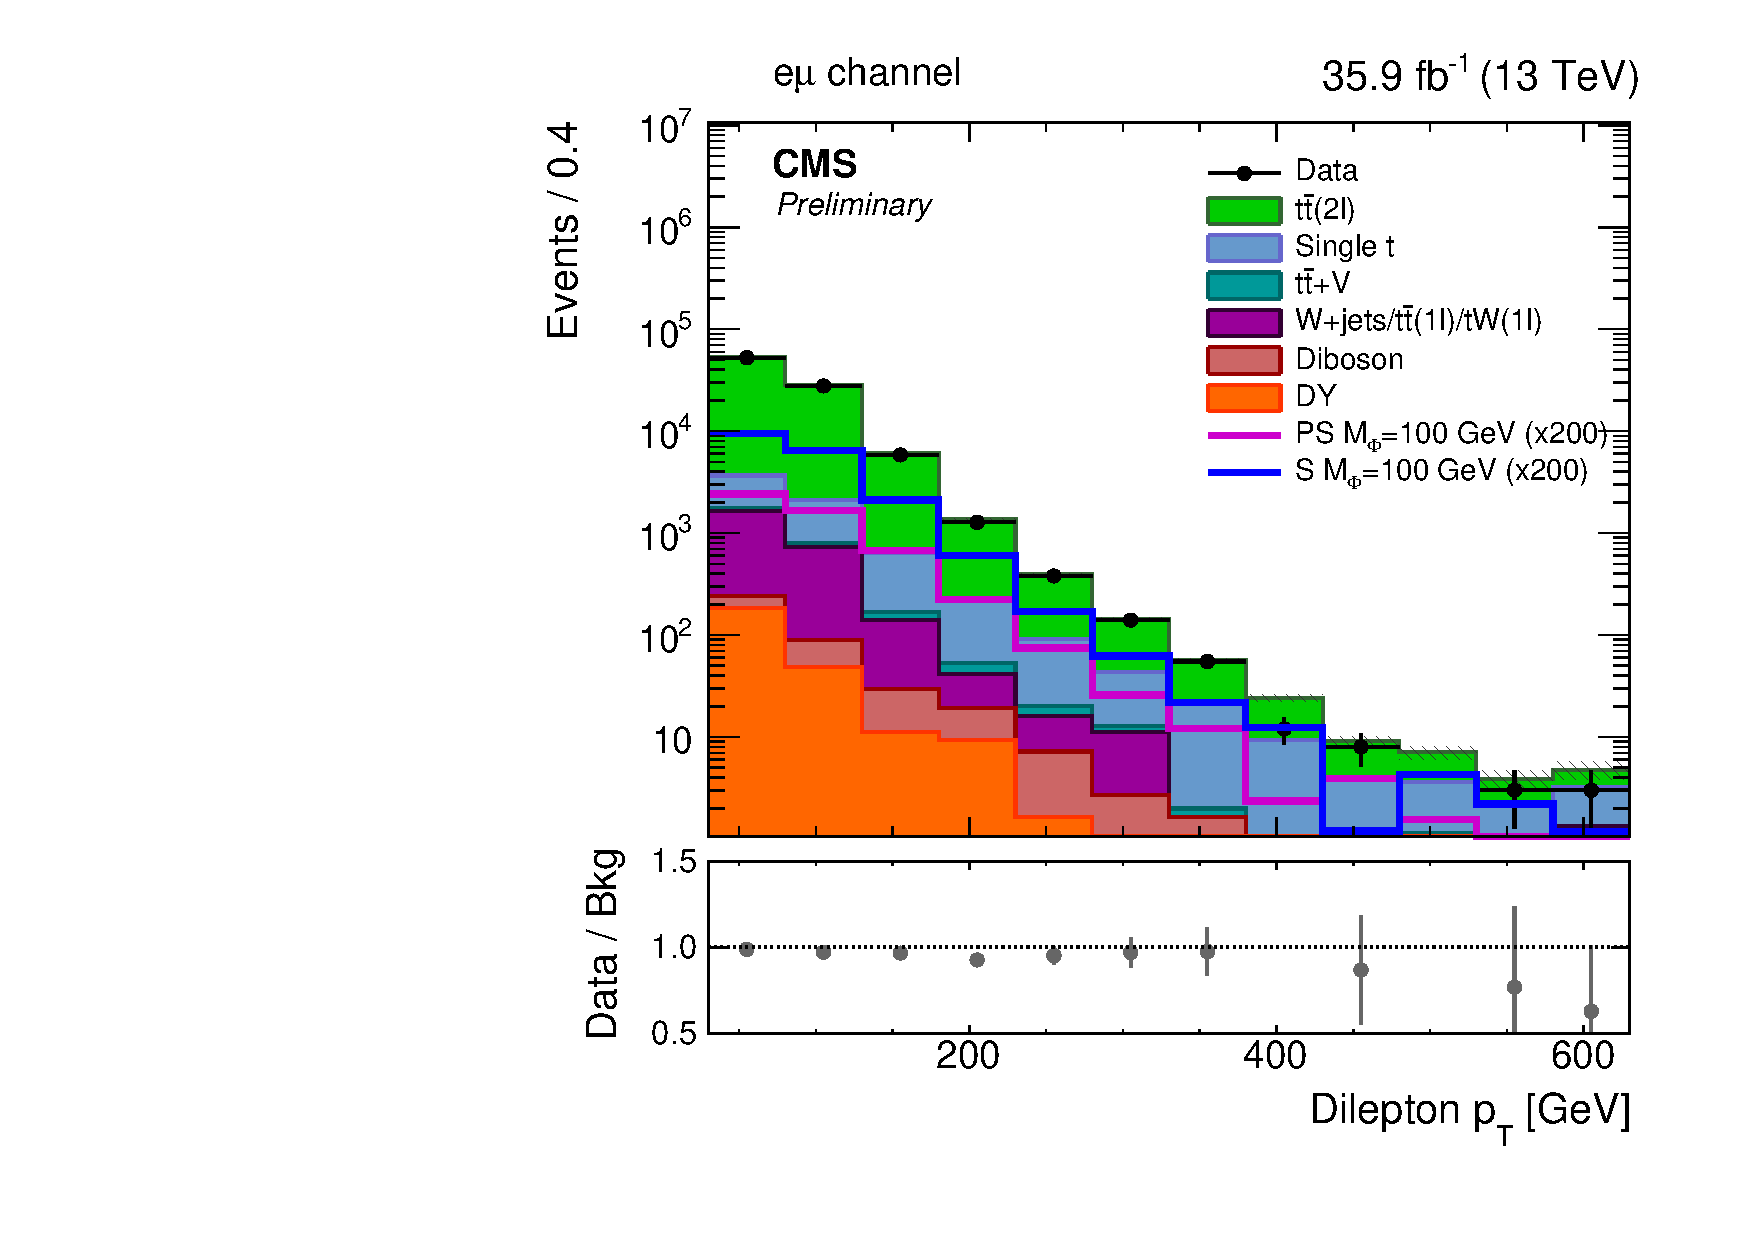
\includegraphics[width=0.45\textwidth]{figs/inclusiveSR/dilepptlog_em.pdf}}
  \subfloat[$m_{\ell\ell}$]                    {\label{subfig:dilepmass_em}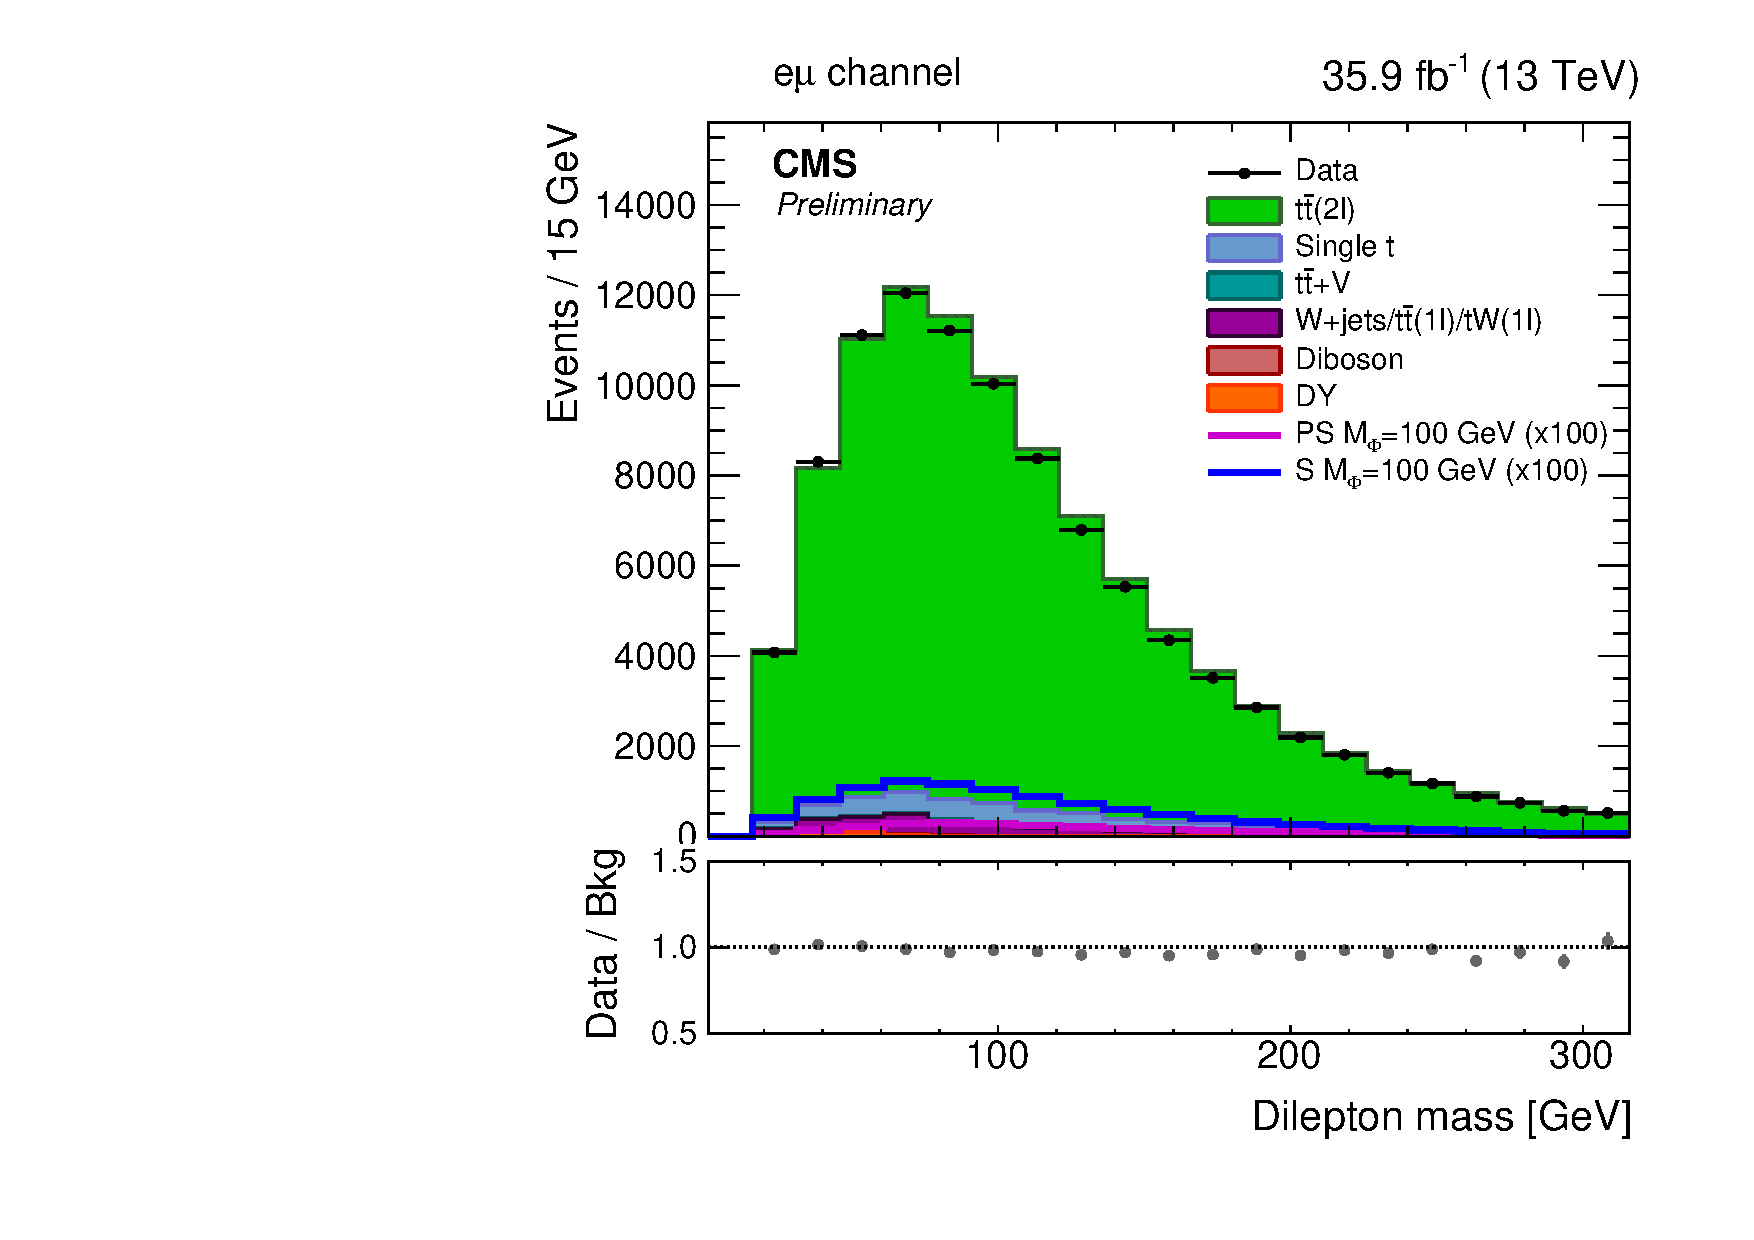
\includegraphics[width=0.45\textwidth]{figs/inclusiveSR/dilepmass_em.pdf}} \\ 
%  \subfloat[$\Delta\phi(\vec{p}_{\text{T}}^{\ell\ell},\ptvecmiss)$] {\label{subfig:dphidilepmet_em}  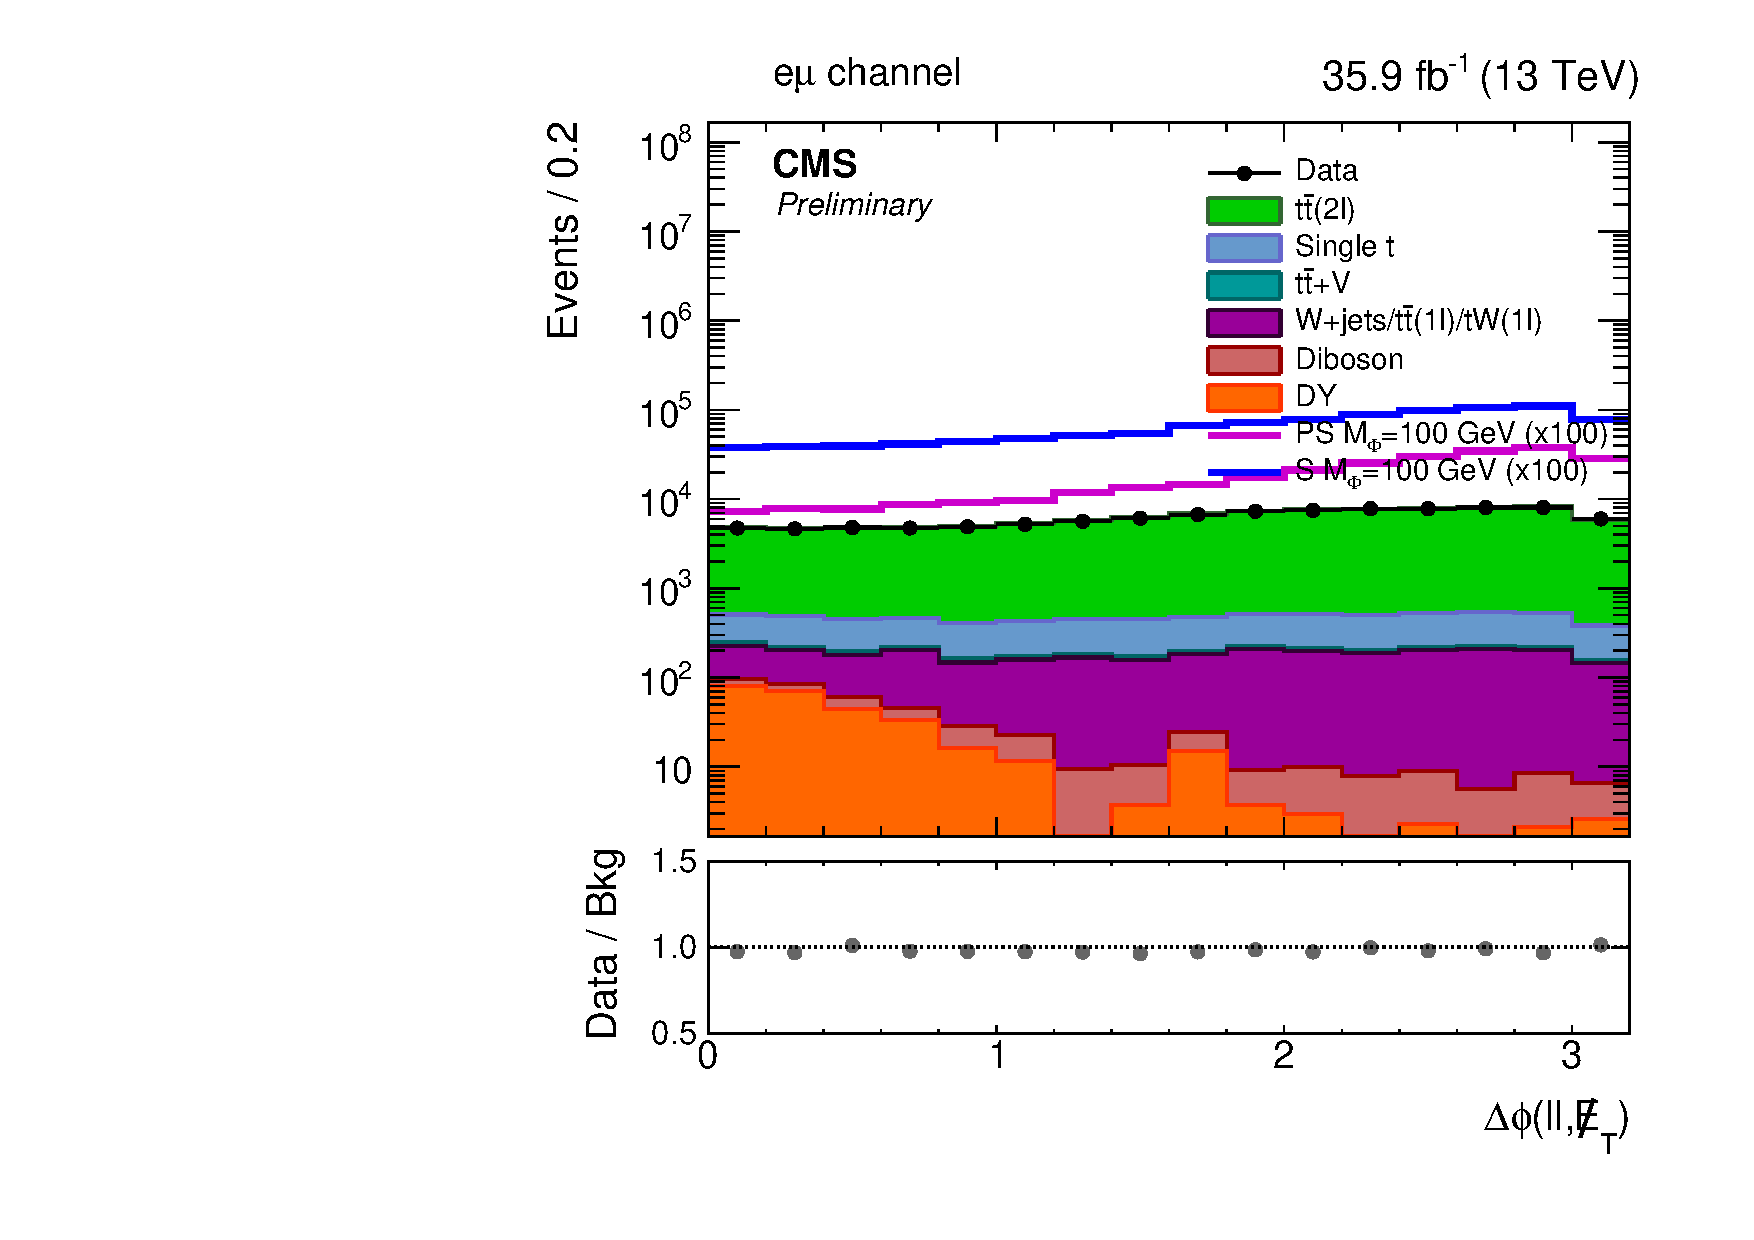
\includegraphics[width=0.4\textwidth]{figs/inclusiveSR/dphidilepmetlog_em.pdf}}
  \subfloat[\ptmiss]                           {\label{subfig:met_em}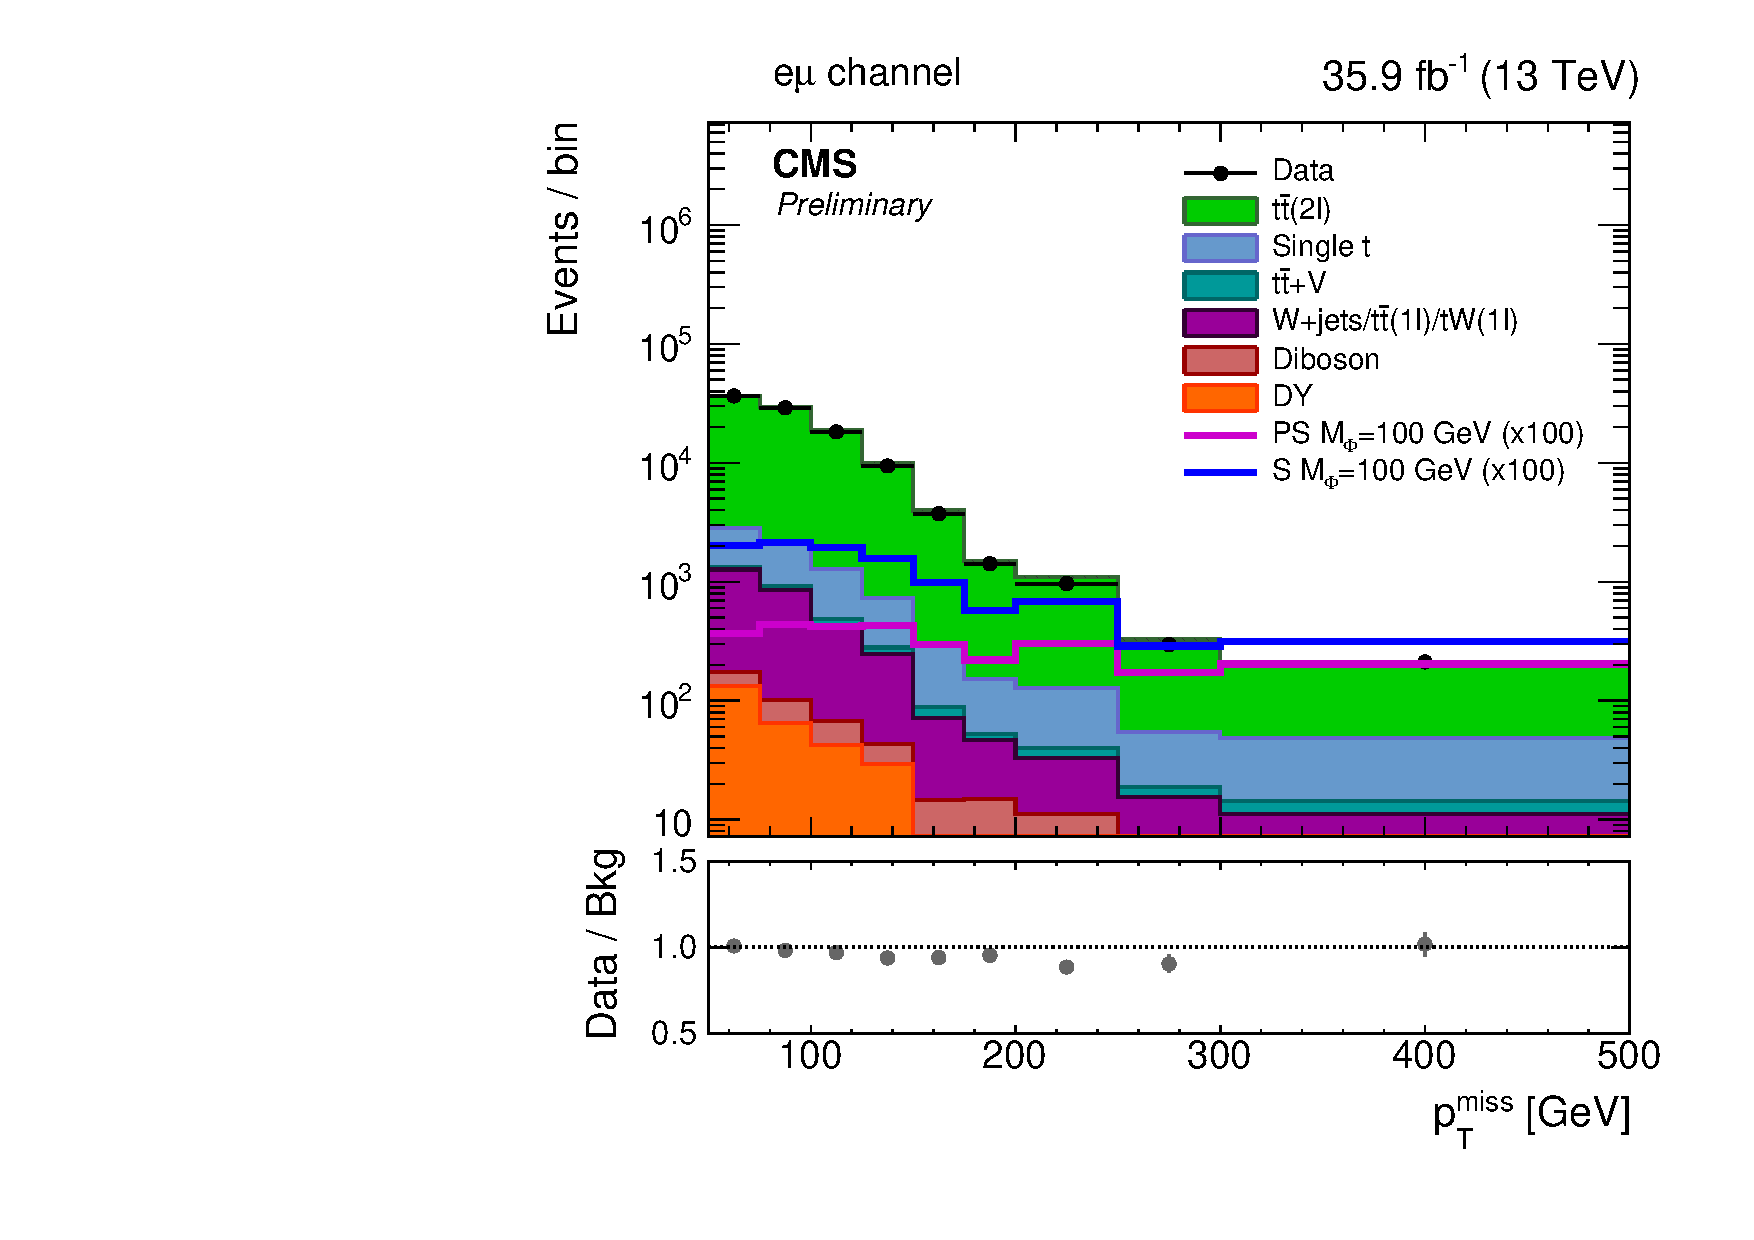
\includegraphics[width=0.45\textwidth]{figs/inclusiveSR/metlog_em.pdf}}
  \caption{Kinematic distributions in the same flavor ($e\mu$) channel. Signals with a pseudoscalar (magenta) and scalar (blue) mediator with $\mMed=100\:\GeV$ and $\mDM=1\:\GeV$ are overlayed and scaled by a factor of 200 to illustrate the potential shape differences between the signal and background in the various distributions. The uncertainties shown in these plots on the data and background are purely statistical.}
  \label{fig:dilep_sr_em}
\end{figure}

\begin{figure}
  \subfloat[][$ee+\mu\mu$ channel] {\label{subfig:mt2ll_sf} 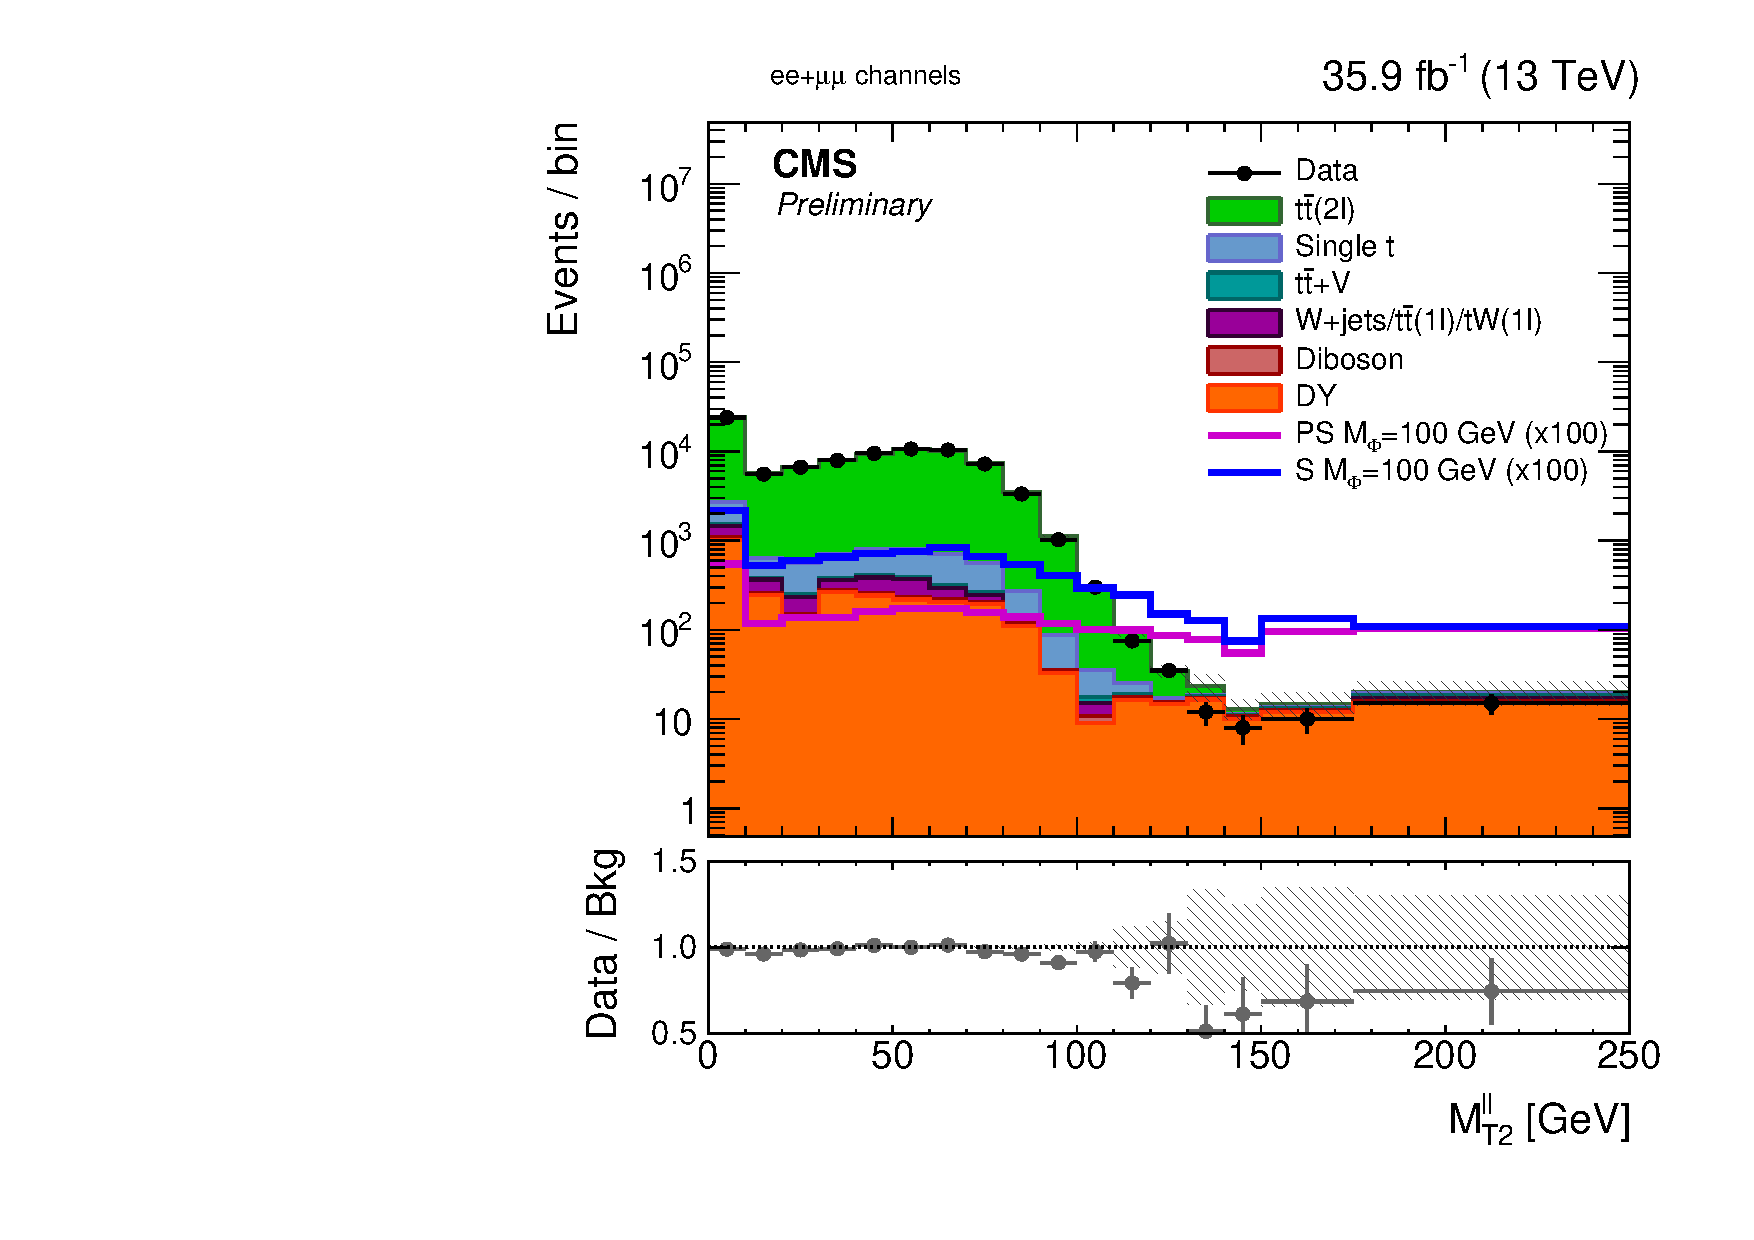
\includegraphics[width=0.48\textwidth]{figs/inclusiveSR/mt2log_sf.pdf}} 
  \subfloat[][$e\mu$ channel]      {\label{subfig:mt2ll_em} 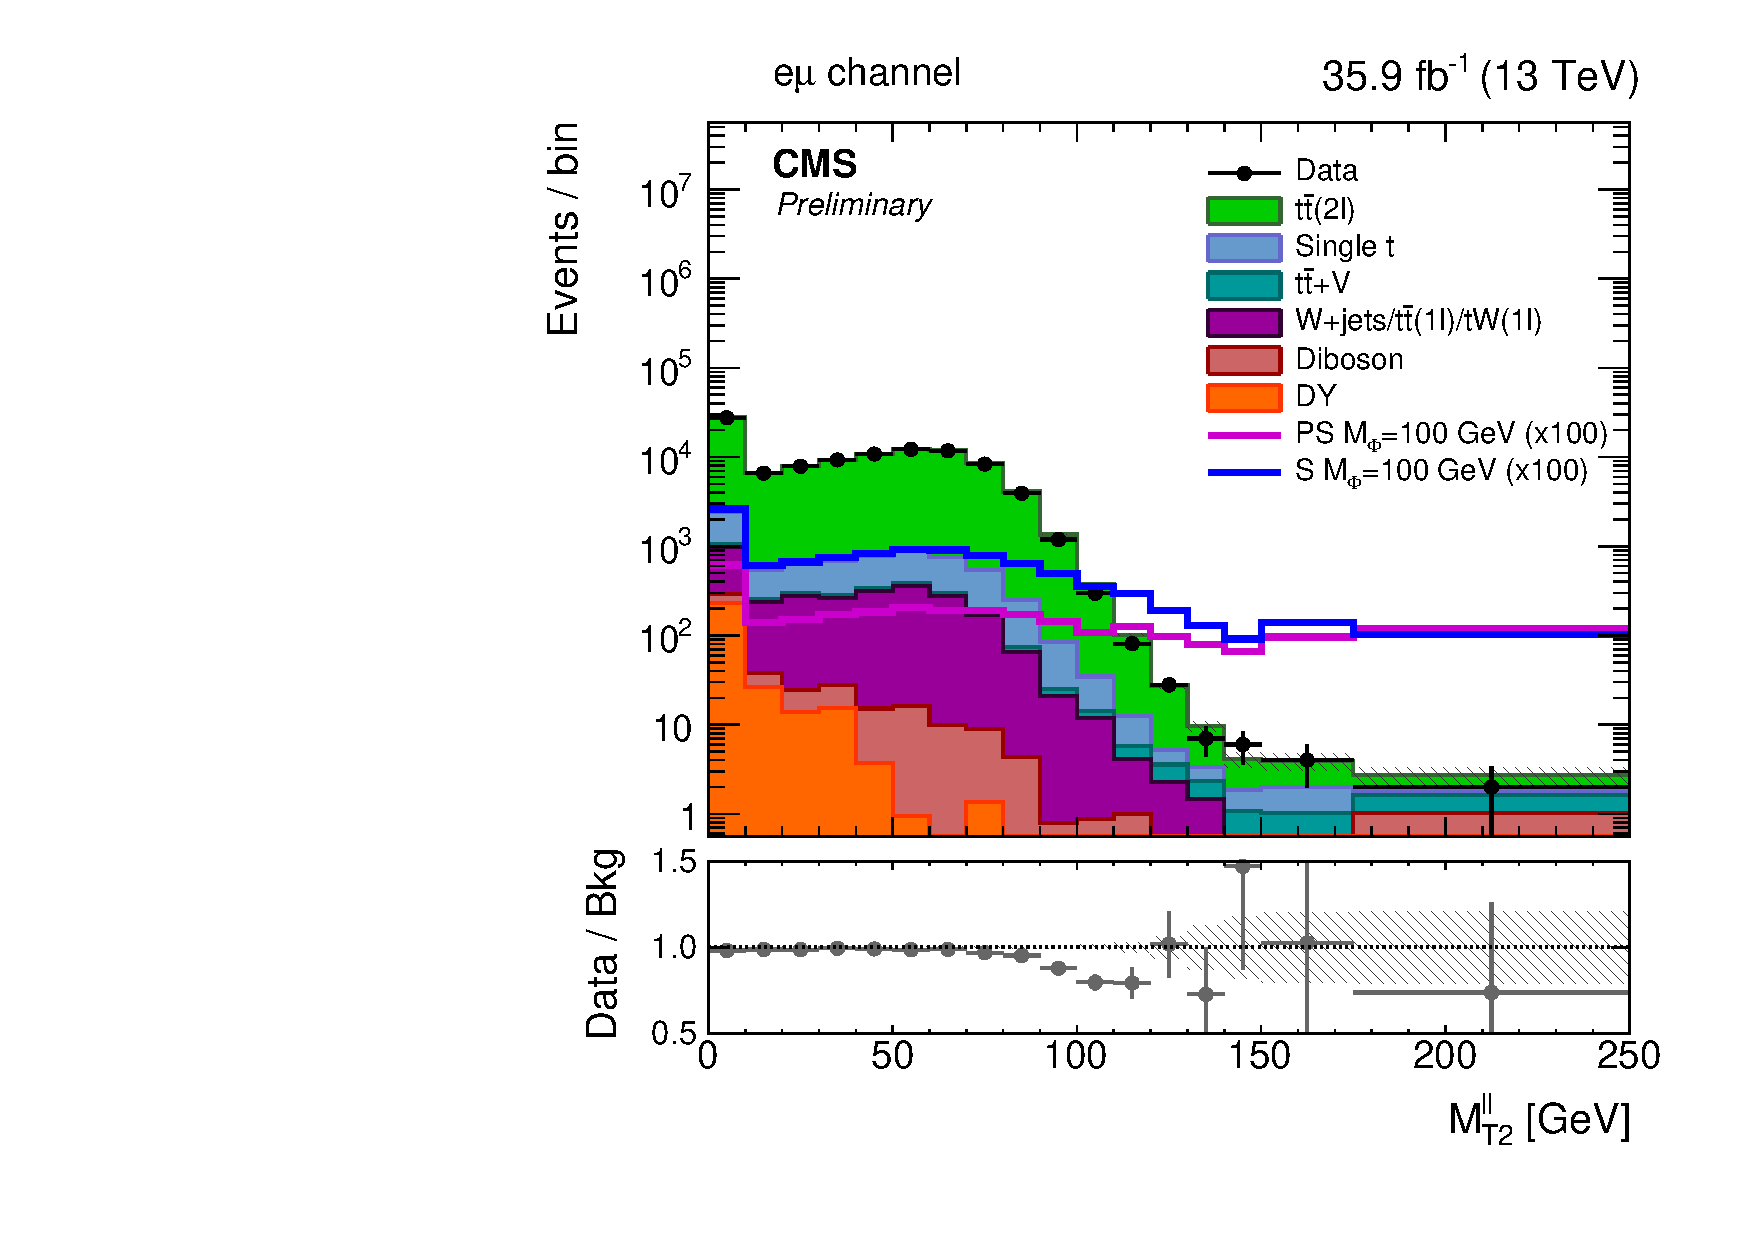
\includegraphics[width=0.48\textwidth]{figs/inclusiveSR/mt2log_em.pdf}} 
  \caption{The \mttll distribution in the~\protect\subref{subfig:mt2ll_sf} same flavor and~\protect\subref{subfig:mt2ll_em} opposite flavor channels. Events with \mttll below (above) $110\:\GeV$ form the low (high) signal purity categories. The uncertainties in the above plots are statistical only. The \mttll templates for signals with a pseudoscalar (magenta) and scalar (blue) mediator with $\mMed=100\:\GeV$ and $\mDM=1\:\GeV$ are overlayed and scaled by a factor of 200.}
  \label{fig:mt2_sr}
\end{figure}

\begin{figure}
  \subfloat[][low purity: $ee+\mu\mu$] {\label{subfig:metlo_sf} 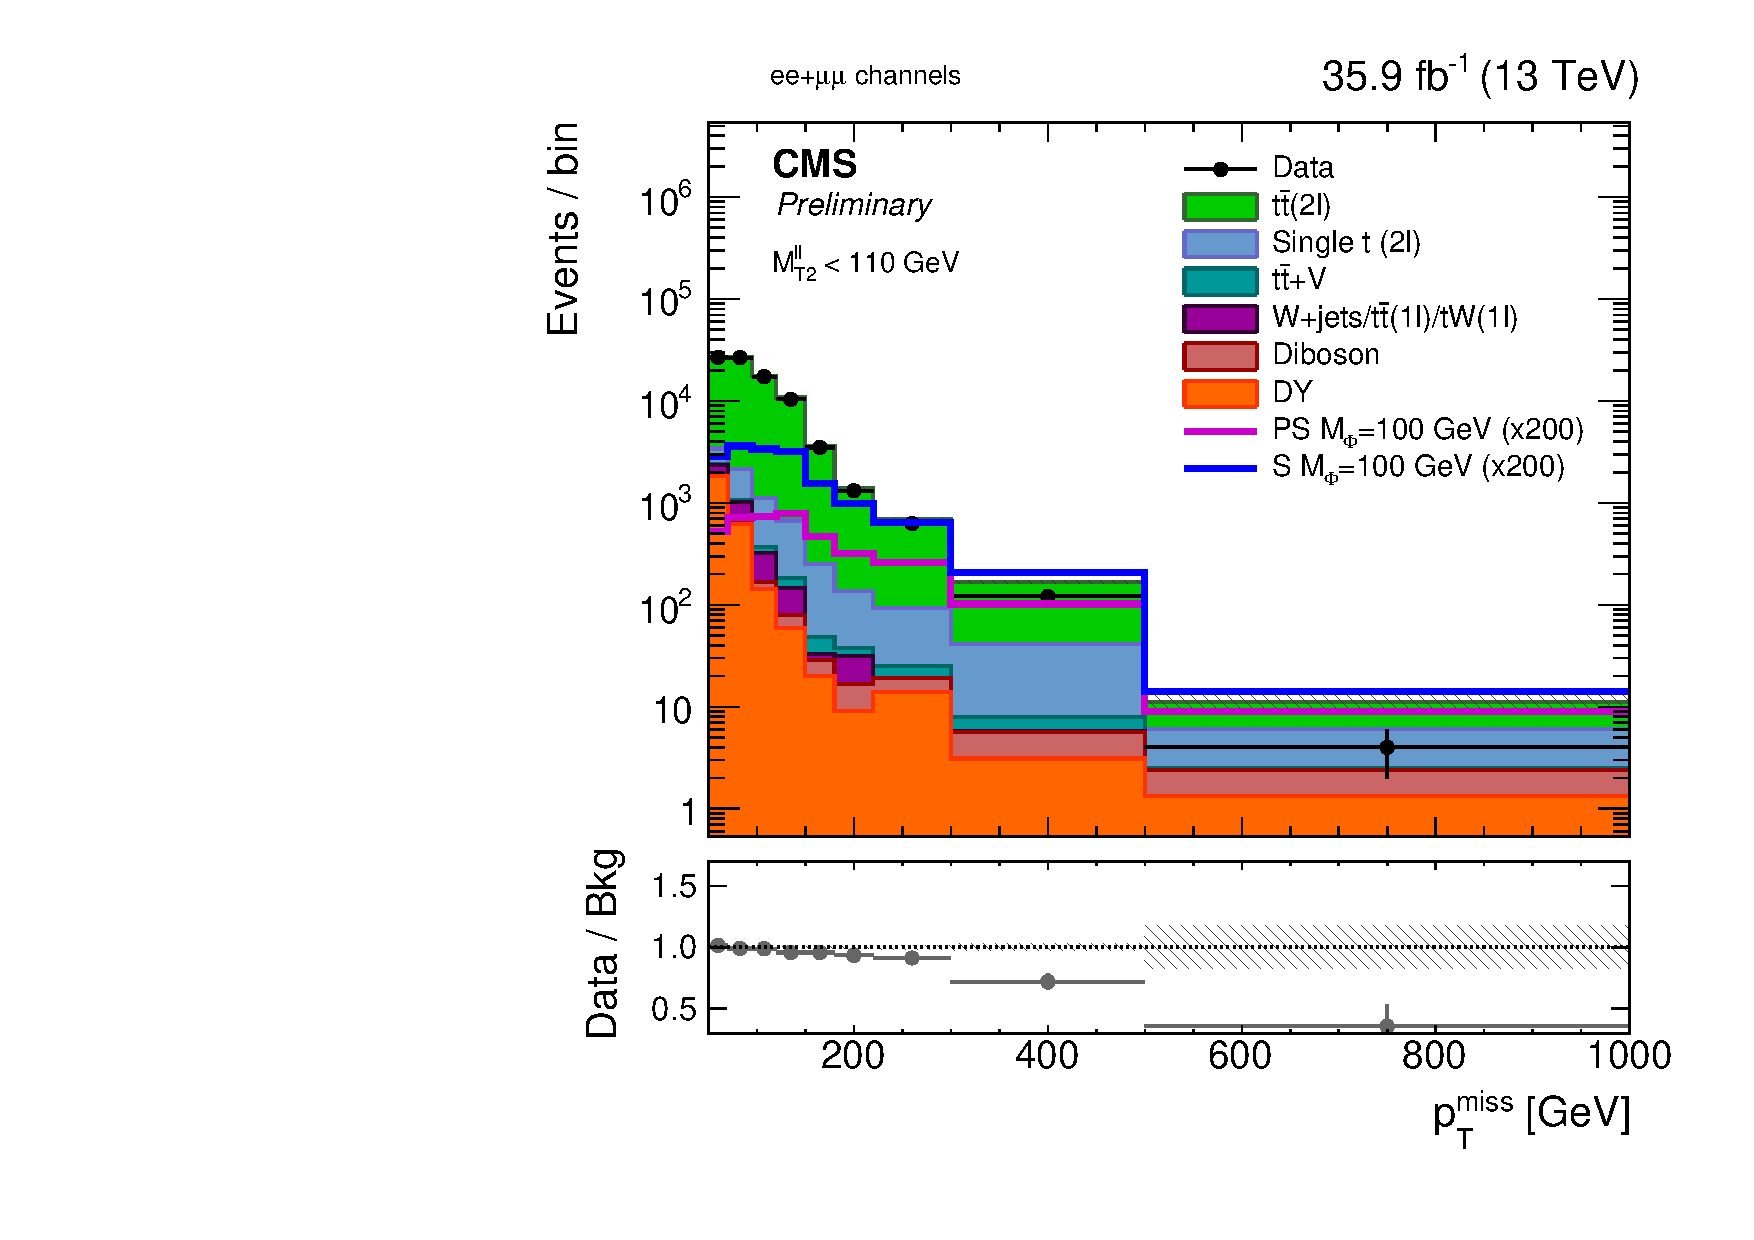
\includegraphics[width=0.48\textwidth]{figs/cat-lo_metlog_ll.pdf}}
  \subfloat[][low purity: $e\mu$]      {\label{subfig:metlo_em} 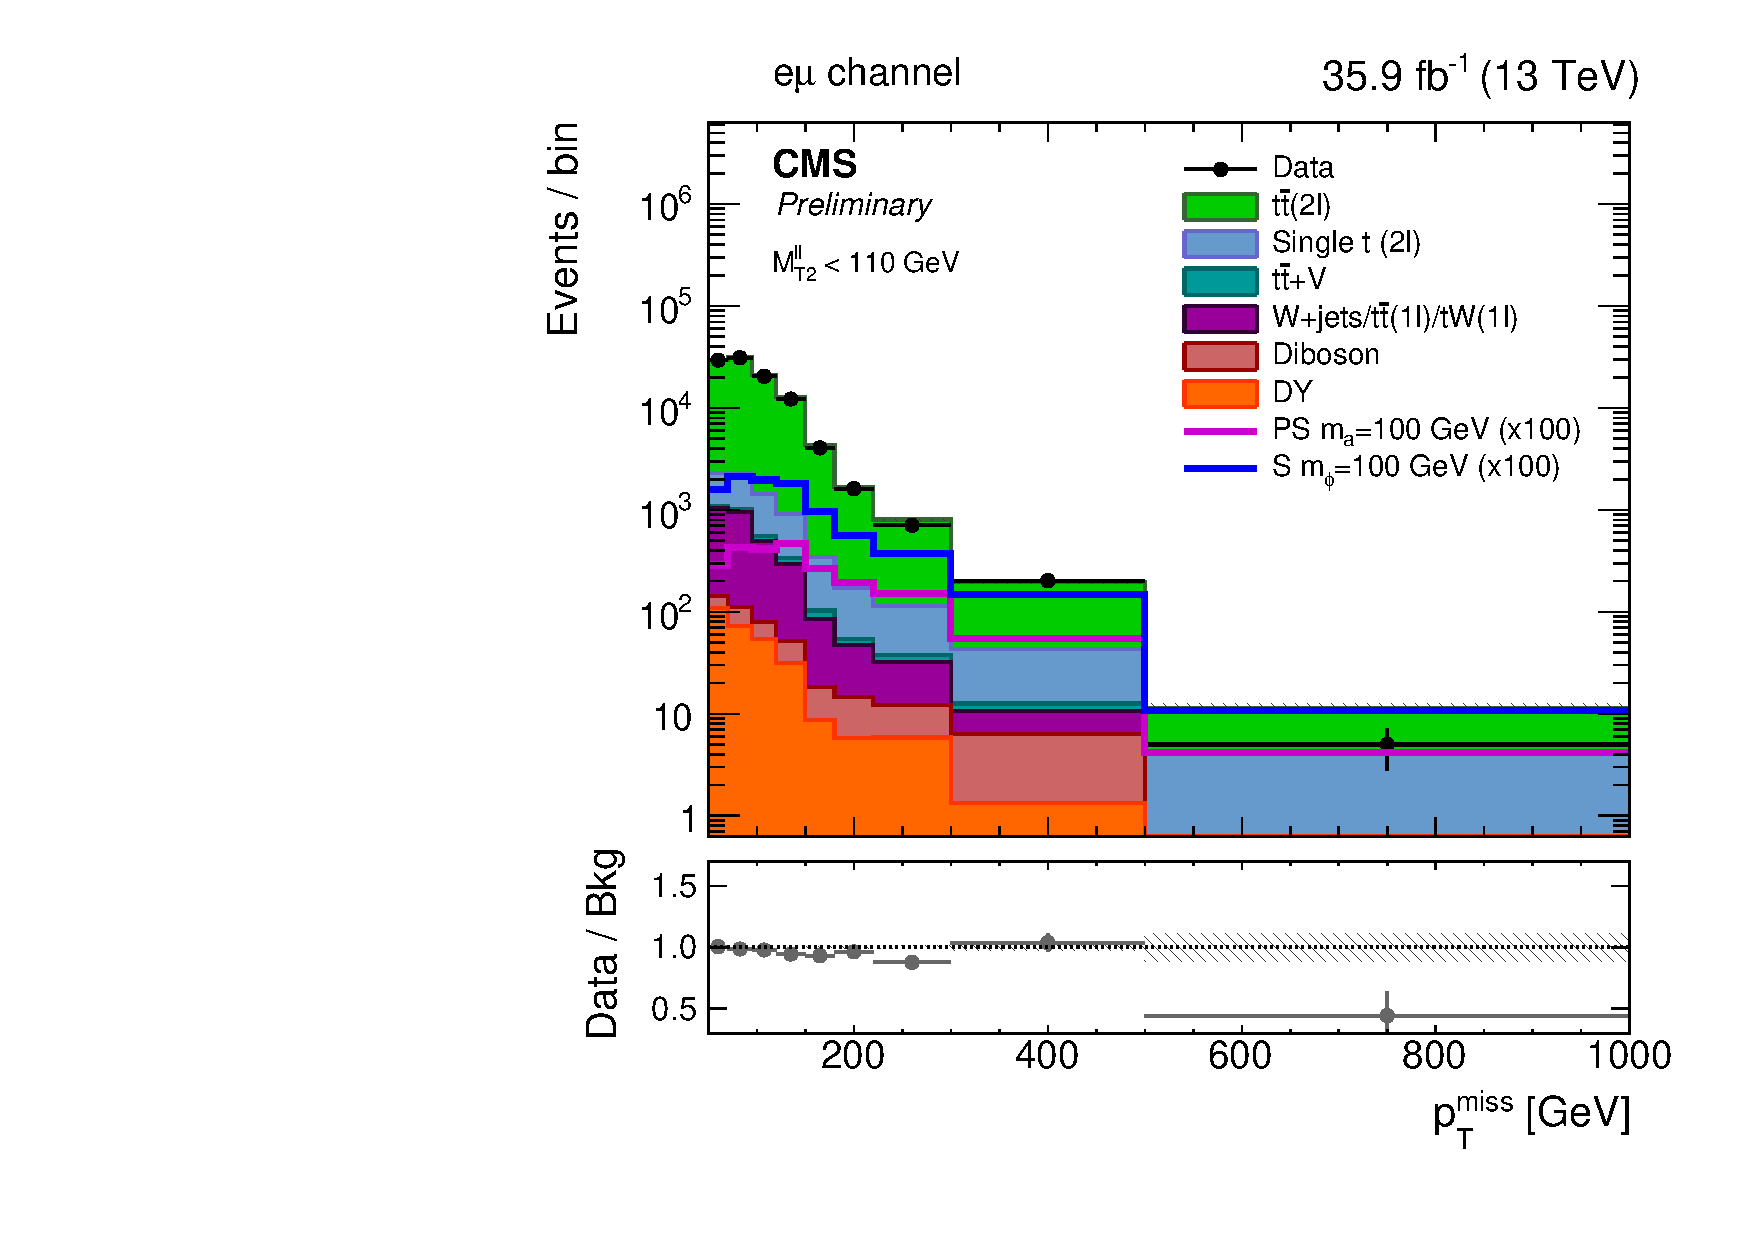
\includegraphics[width=0.48\textwidth]{figs/cat-lo_metlog_em.pdf}}
  \caption{The \ptmiss distributions in the low purity signal region for~\protect\subref{subfig:metlo_sf} same flavor and~\protect\subref{subfig:metlo_em} opposite flavor events. The uncertainties in the above plots are statistical only. The \ptmiss templates in the low purity signal region for signals with a pseudoscalar (magenta) and scalar (blue) mediator with $\mMed=100\:\GeV$ and $\mDM=1\:\GeV$ are overlayed and scaled by a factor of 200.}
  \label{fig:metlo}
\end{figure}

\begin{figure}
  \subfloat[][high purity: $ee+\mu\mu$] {\label{subfig:methi_sf} 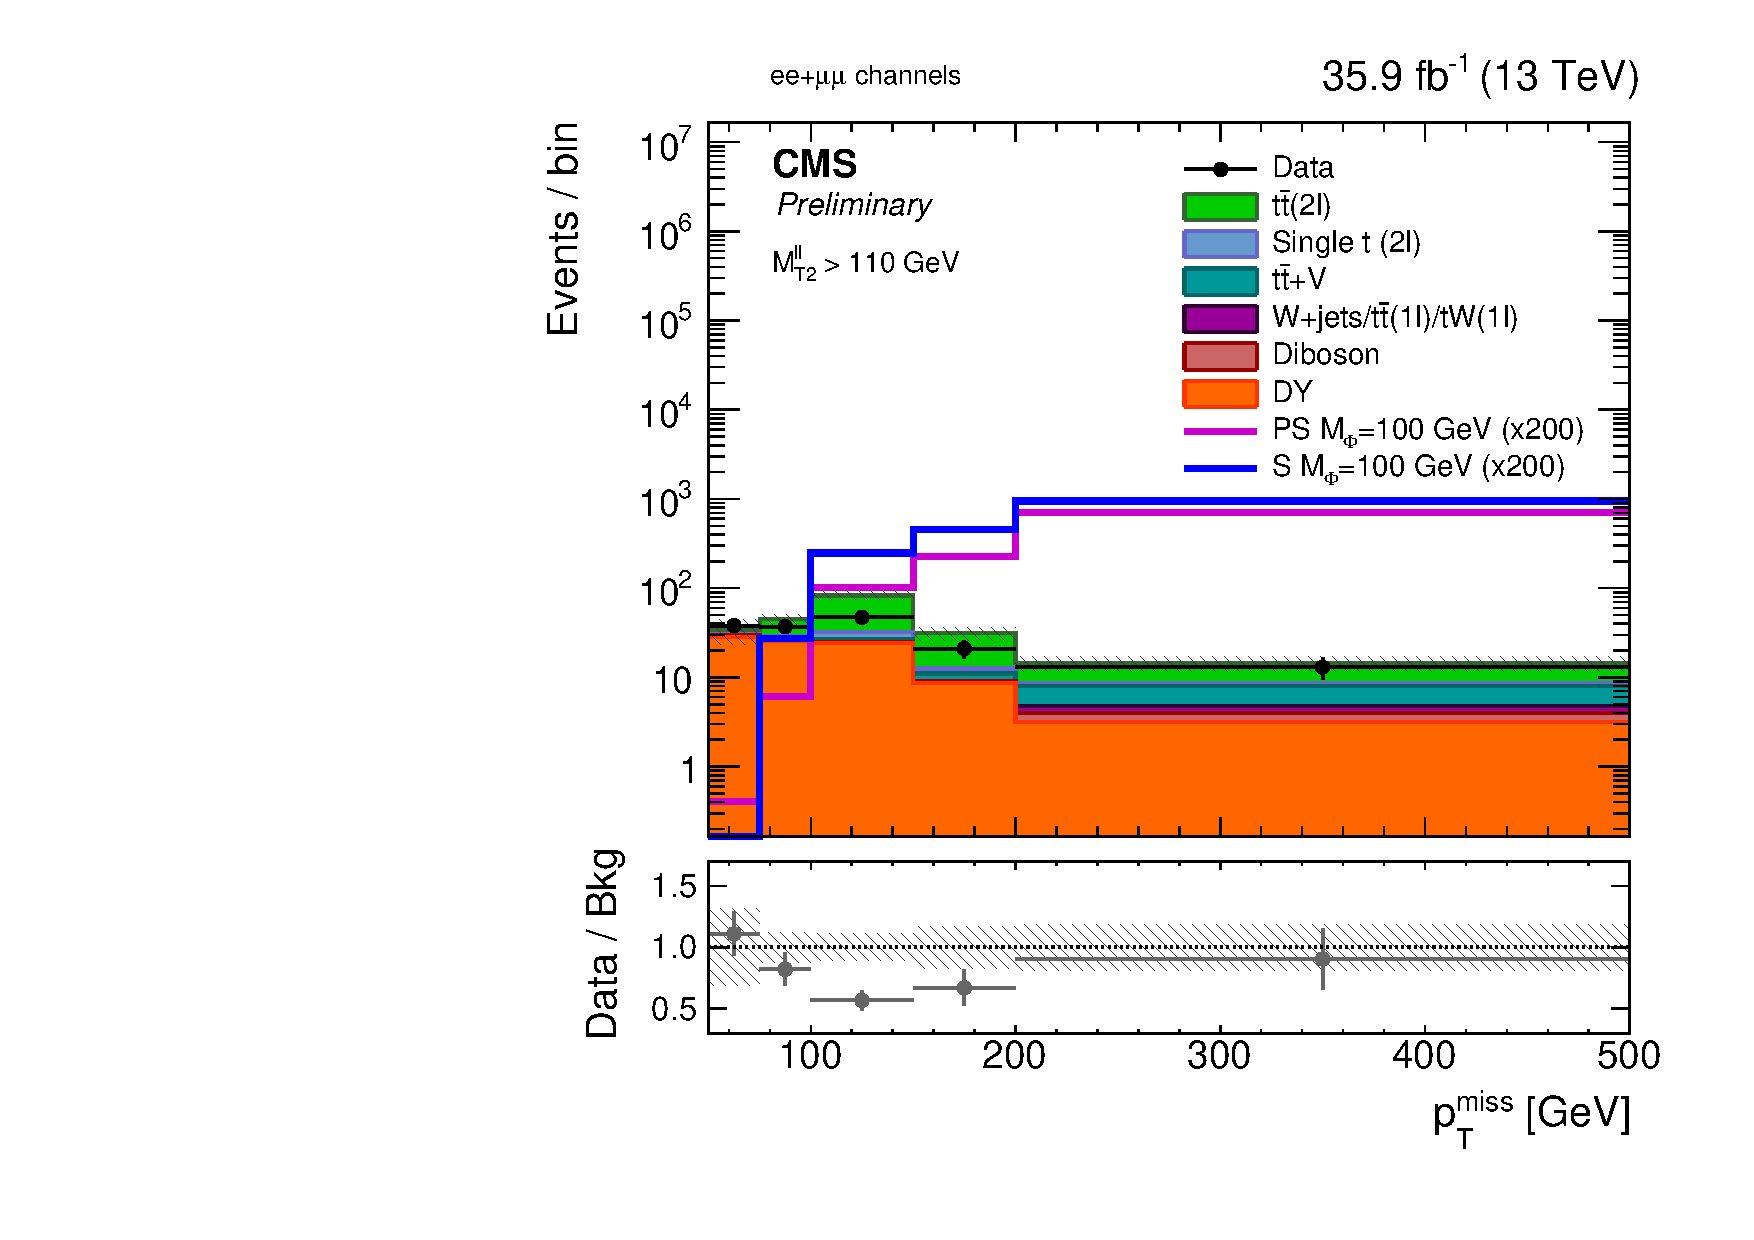
\includegraphics[width=0.48\textwidth]{figs/cat-hi_metlog_ll.pdf}}
  \subfloat[][high purity: $e\mu$]      {\label{subfig:methi_em} 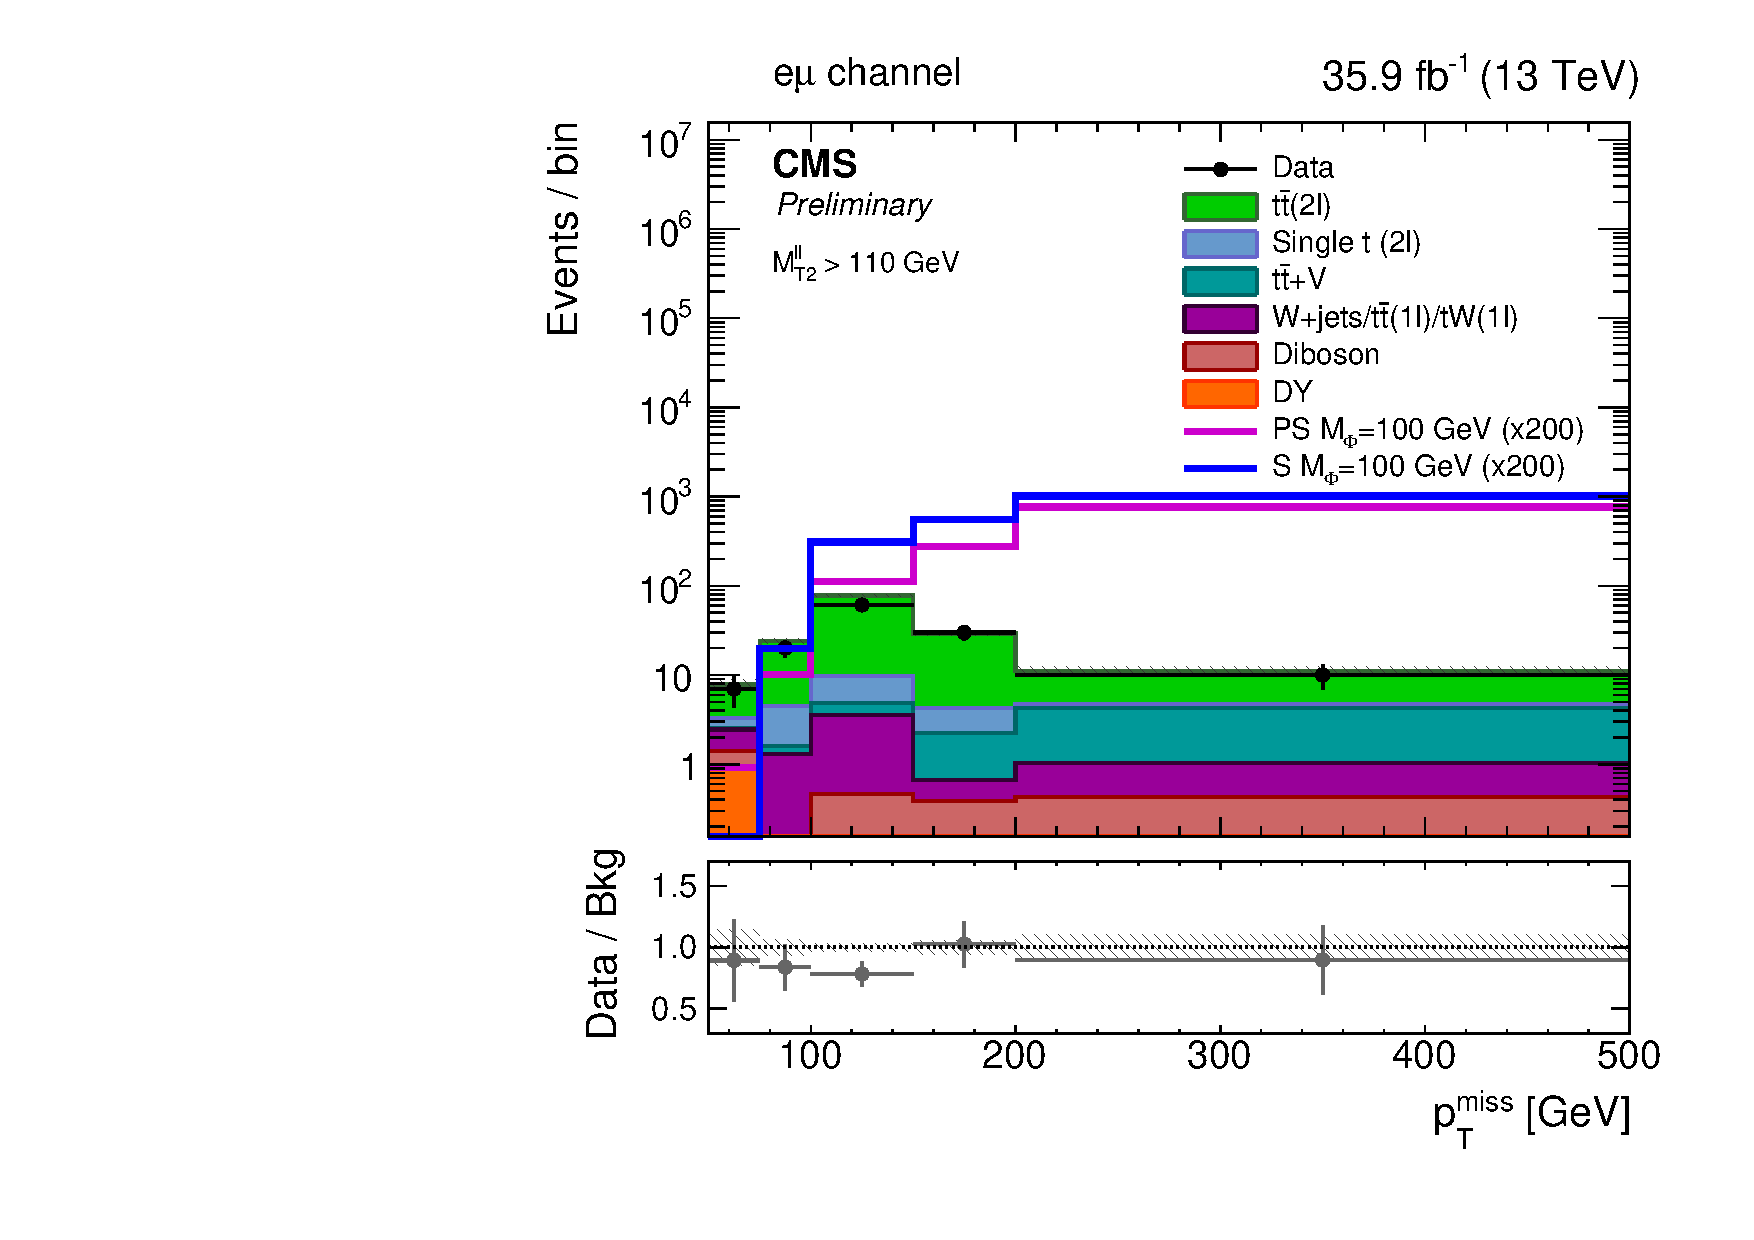
\includegraphics[width=0.48\textwidth]{figs/cat-hi_metlog_em.pdf}}
  \caption{The \ptmiss distributions in the high purity signal region for~\protect\subref{subfig:methi_sf} same flavor and~\protect\subref{subfig:methi_em} opposite flavor events. The uncertainties in the above plots are statistical only. The \ptmiss templates in the high purity signal region for signals with a pseudoscalar (magenta) and scalar (blue) mediator with $\mMed=100\:\GeV$ and $\mDM=1\:\GeV$ are overlayed and scaled by a factor of 200.}
  \label{fig:methi}
\end{figure}


\section{Systematic uncertainties}
\label{sec:systunc}

The signal and background \ptmiss templates derived from simulation are subject to effects incurred from experimental and theoretical sources of uncertainty. The \ptmiss distributions are parametrized in order to allow for constrained shape and normalization variations as a cause of the systematic uncertainties, referred to throughout as ``systematics''. Each systematic is represented by a nuisance parameter, $\theta$, with a probability density function, $pdf$, denoted as $\rho(\theta)$, that contains the central value of the nuisance, $\widetilde{\theta}$, and other parameters that describe the overall shape of the $pdf$, such as its width. 

Uncertainties which affect the normalization of the signal and background processes are modeled using nuisance parameters with log-normal probability densities. The log-normal $pdf$ follows the form~\cite{CMS-NOTE-2011-005},

\begin{equation}
  \rho(\theta) = \frac{1}{\sqrt{2\pi}\ln{\kappa}}\exp{\bigg(-\frac{(\ln{(\theta/\widetilde{\theta})})^2}{2(\ln{\kappa})^2}\bigg)}\frac{1}{\theta}.
\end{equation}

where the width of the log-normal distribution is characterized by $\kappa$, and $\widetilde{\theta}$ represents the best estimate of the nuisance $\theta$. In the limit of small uncertainty ($\epsilon$), the width of a Gaussian $pdf$ is given by $\sigma=\epsilon$, which equates directly to the log-normal width via a Taylor expansion for $\kappa = e^{\epsilon}$, such that $\kappa=1+\epsilon$. The log-normal $pdf$ is useful in the case of large uncertainties as the distribution has a longer tail in comparison with a Gaussian $pdf$, and avoids the problem of negative parameter values obtained from a Gaussian probability density, since $\rho(\theta)\rightarrow0$ as $\theta\rightarrow0$.

A number of uncertainties influence the overall shape of the signal and background \ptmiss templates along with the normalization. Systematics of this type are implemented using a general technique known as ``vertical morphing''~\cite{Conway:2011in}. A change in a particular type of uncertainty (such as an energy scale) can cause a distortion in both the shape and overall normalization of the efficiency as a function of the observable (\ptmiss) bin. Raising and lowering a particular parameter to its corresponding values at one standard deviation will cause the bin efficiencies, denoted as $\epsilon_{ij}$ for source $i$ in observable bin $j$, to also shift, thus resulting in three measures of the bin efficiency shape, referred to as $\epsilon^{+}_{ij}$, $\epsilon^{0}_{ij}$, and $\epsilon^{-}_{ij}$. In order to transform the three shape measures into a continuous estimate as a function of the parameter value, a morphing parameter, represented by $f$ and nominally equal to 0 with a unitary uncertainty, is used. A quadratic interpolation is used for values where $|f|<1$, to express the efficiency in a bin as a function of the morphing parameter such that, 

\begin{equation}
  \epsilon_{ij} = \frac{f(f-1)}{2}\epsilon^{-}_{ij} - (f-1)(f+1)\epsilon^{0}_{ij} + \frac{f(f+1)}{2}\epsilon^{+}_{ij}.
  \label{eq:morph}
\end{equation}

The form of Eq.~\ref{eq:morph} guarantees that the value of the expression is $\epsilon^{\pm}_{ij}$ for $f=\pm 1$. In the case that a nuisance parameter is shifted by more than one standard deviation from its nominal value and thereby resulting in efficiency values in the range $|f|>1$, a linear extrapolation is performed.

\subsection{Sources of systematic uncertainty}
\label{subsec:sources}
The following sources of uncertainty affect the normalization of the signal and background processes: 

\begin{itemize}
  \item \textbf{Pileup modeling}: As described in \SectionRef{subsec:pu}, the total inelastic cross section used to calculate the data pileup distributions is varied by $\pm4.6\%$, in order to account for systematic uncertainties due to pileup modeling. Normalization differences in the range of $0.3-11\%$ across the different physics processes result from reweighting the simulation accordingly.
  \item \textbf{Integrated luminosity}: The overall uncertainty of the measurement of the integrated luminosity delivered to the CMS Experiment during the 2016 LHC pp run at $\sqrt{s}=13\:\TeV$ is estimated to be $2.5\%$~\cite{CMS-PAS-LUM-17-001}.
  \item \textbf{Lepton reconstruction and selection}: The uncertainty on lepton reconstruction and selection efficiency is associated with the efficiency measurement with samples of Z bosons decaying to dielectrons or dimuons~\cite{CMS:2011aa}. The $\pt$- and $\eta$-dependent scale factors are varied within their uncertainties which amounts to $\approx 2\%$ per lepton.
  \item \textbf{Lepton trigger}: The uncertainty on lepton triggering efficiency is associated with the efficiency measurement with samples of Z bosons decaying to dielectrons or dimuons. For muon triggers, the uncertainties across physics processes for both low and high \mttll SRs are approximately $2\%$ in the SF and $1.5\%$ in the OF categories. Analogously, the uncertainties for electron triggers are approximately $1.8\%$ in the SF and $2.2\%$ in the OF categories. 
  \item \textbf{b-tagging efficiency}: The b-tagging efficiency and mis-tag rate and the respective uncertainties are measured on independent control samples. Uncertainties from gluon splitting, the b quark fragmentation function, and the selections used to define the control samples are propagated to the efficiency scale factors~\cite{CMS-PAS-BTV-15-001}. The uncertainties on the mis-tag rate range from $0.1-4\%$, while the b-tagging efficiency uncertainties range from $0.1-2\%$, across physics processes across all categories where the largest uncertainty is incurred in the low \mttll category for the diboson background.
  \item \textbf{Single top and diboson normalization}: In practice, the expected yields for background processes are either scaled to data or to theory predictions with the best available accuracy. The PDF and the renormalization and factorization scale variations take into account the uncertainties on the background acceptances. However, in the single top and diboson simulation samples used, the aforementioned variations are not available, so a conservative uncertainty of $20\%$ and $10\%$ is assigned respectively to the normalizations, and these uncertainties are treated independently of eachother.  
\item \textbf{Drell-Yan background uncertainty}: The uncertainties incurred from the data-driven estimate of the Drell-Yan background normalization are dominated by the statistical uncertainties on $N_{\mbox{\tiny{in}}}$ and $R^{1b}_{\mbox{\tiny{MC}}}$, quantities used to extrapolate yields from a region near the Z boson mass to regions away from it, as described in \SectionRef{sec:DY}. The uncertainties are $11\%$ and $6\%$ for the $ee$ and $\mu\mu$ channels and only applies to the DY background in the SF regions.
\item \textbf{Fake lepton background uncertainty}:
The sources of uncertainty in the fake lepton background stem from the uncertainty in the measured fake rate, and from the statistical uncertainty of the single-lepton application sample to which the rate is applied, as described in \SectionRef{sec:fakes}. The uncertainties are $78\%$ ($ee$), $70\%$ ($e\mu$), $74\%$ ($\mu\mu$) in the high signal purity category and $47\%$ ($ee$), $12\%$ ($e\mu$), and $20\%$ ($\mu\mu$) in the low signal purity category, and are dominated by the statistical uncertainty associated with the single-lepton application sample. Since the fake lepton background is small, these relatively large uncertainties do not significantly degrade the sensitivity of the search.
\end{itemize}

The systematics affecting the overall \ptmiss shape and normalization are listed below in order of decreasing dominance on the final result. For some systematics, the changes in the \ptmiss spectra as a result of the $\pm 1\sigma$ uncertainty variation has been shown for pertinent processes. A full suite of such experimental plots for all systematics affecting the \ptmiss templates derived for various signal and background processes can be found in ~\AppendixRef{}.

\begin{itemize}
  \item \textbf{Jet energy scale (JES)}: The reconstructed energy of every jet in an event taken from simulation is varied simultaneously by one standard deviation of the JES uncertainty of the corresponding jet above and below the nominal energy. These JES uncertainties are coherently propagated to all observables impacted, including the jet \pt, jet multiplicity, \ptmiss, and \mttll.~\FigureRef{fig:JESshape} shows an example of the effect on the SM \ttll \MET templates in the high and low \mttll-SF region after variation by $\pm1\sigma$ of the JES uncertainty, as represented by the dashed red ($+1\sigma$) and blue ($-1\sigma$) shapes. Uncertainty effects due to the jet energy resolution (JER) were found to be negligible.

    \begin{figure}[h]
      \centering
      \subfloat[][\ttll, low \mttll-OF]{\label{subfig:JESlo}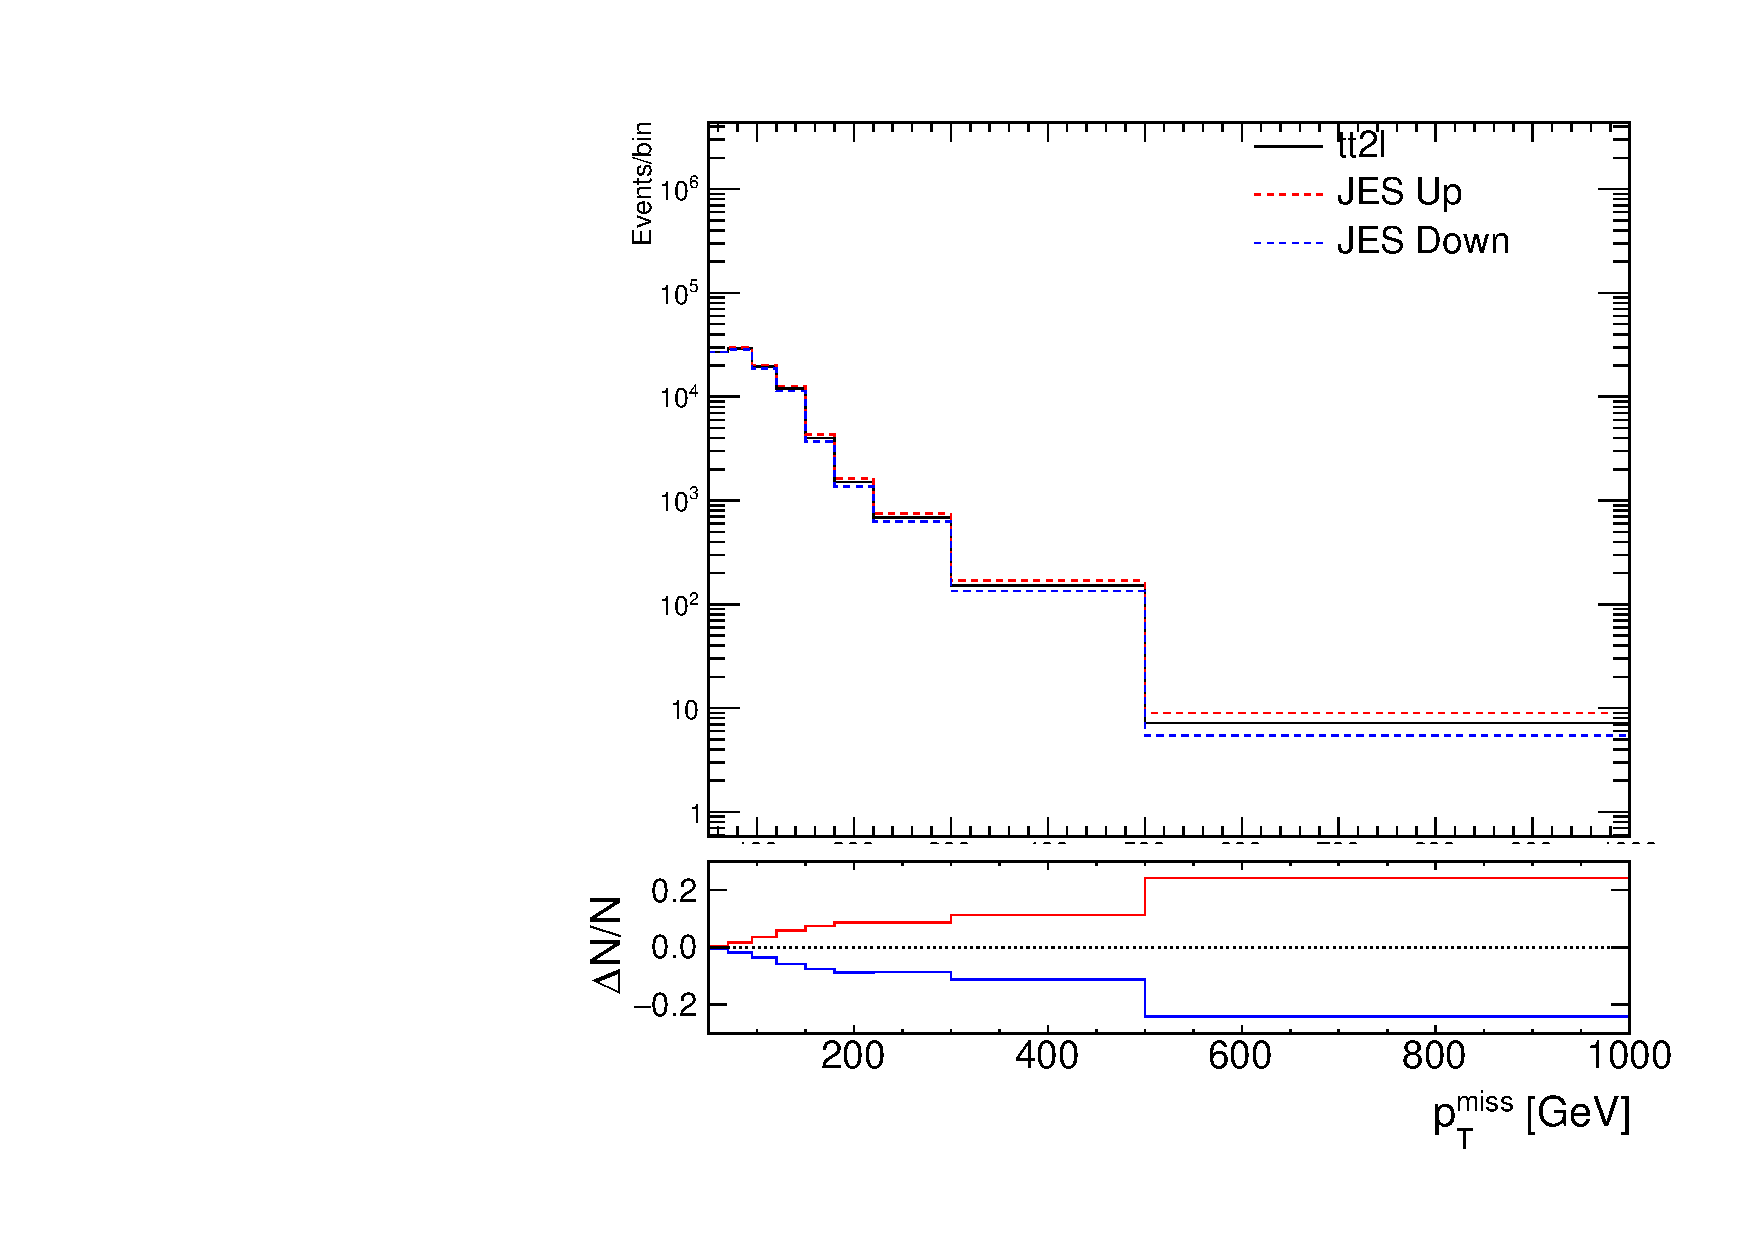
\includegraphics[width=0.48\textwidth]{systs/shapes_ttdm805101_em_lo/tt2l_CMS_scale_j}}
      \subfloat[][\ttll, high \mttll-OF]{\label{subfig:JEShi}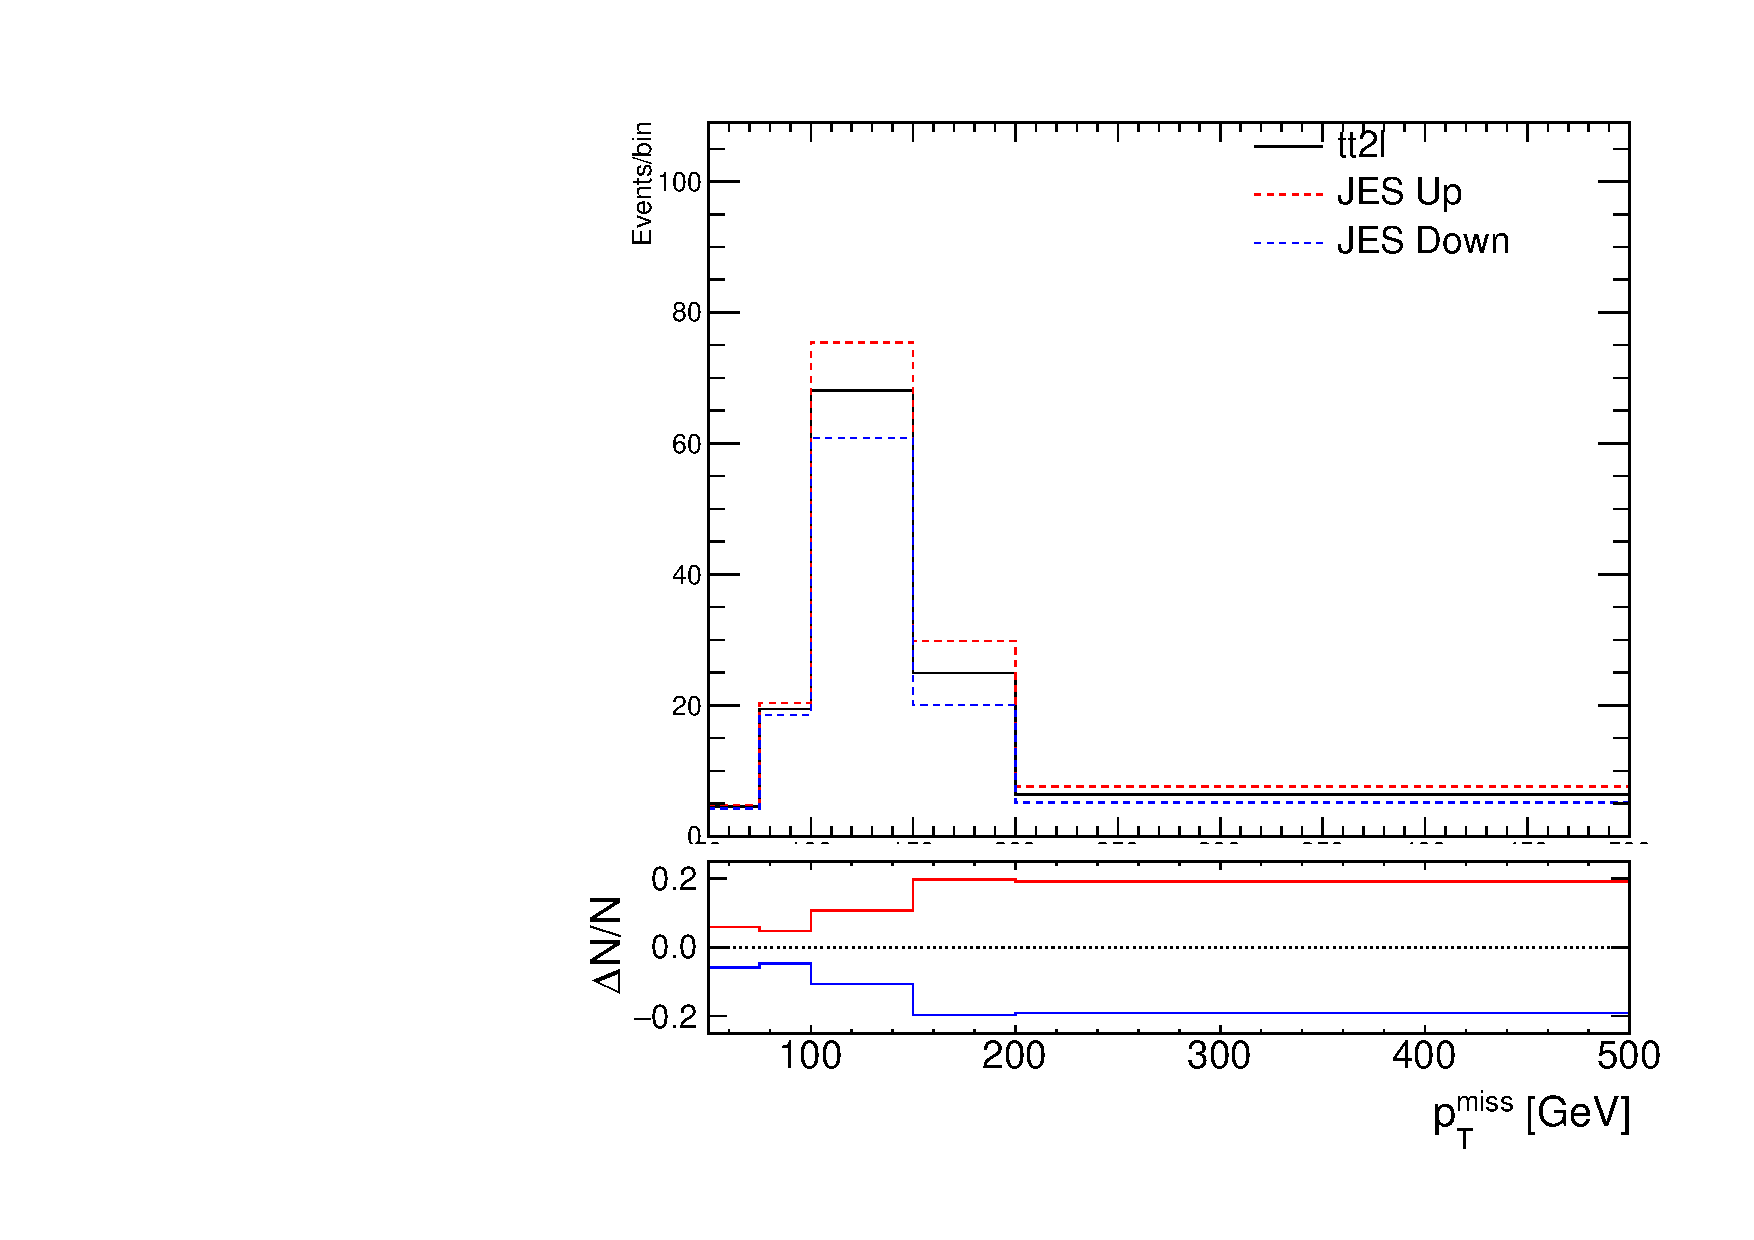
\includegraphics[width=0.48\textwidth]{systs/shapes_ttdm805101_em_hi/tt2l_CMS_scale_j}}
      \caption{The variation in the \ptmiss spectra for \ttll in the low and high \mttll-OF SRs due to the variation of the JES uncertainty by $+1\sigma$ (red) and $-1\sigma$ (blue). The normalized residuals of the ``up'' and ``down'' shapes are shown in the lower panel.}
      \label{fig:JESshape}
    \end{figure}

\item \textbf{Fake \ptmiss uncertainty}: As discussed in \SectionRef{subsec:mt2ll}, in perfect conditions, the SM \ttll contribution should be suppressed below $M_W$, however in practice, the mismeasurement of \ptmiss is possible as a result of jet and lepton detector misreconstruction effects. Hence, SM \ttll events with large values of ``fake'' \ptmiss leak into the high \mttll SRs. Similarly, although genuine sources of \ptmiss are not expected in DY events, lepton mismeasurements lead to an observed ``fake'' \ptmiss in such events. Thus, in the high \mttll-SF and \mttll-OF categories, an uncertainty is assigned to the background \ptmiss shapes derived from simulation to account for potential mismodeling of the rate of events with large fake \ptmiss in simulation. This uncertainty is derived using Z bosons decaying to dielectrons and dimuons, as a function of hadronic recoil (i.e. \ptmiss with the two leptons removed), and also passing $\mttll > 110\:\GeV$. The difference between the simulation and data after the subtraction of non-DY events as expected from simulation, is taken as the uncertainty and added/subtracted to the nominal recoil distribution to obtain the one standard deviation variations. A second-order polynomial is fit to the fake \ptmiss uncertainty scale factor distributions in an effort to smoothen the uncertainty as a function of the recoil, as shown in ~\FigureRef{fig:recoilSF}. The effect on the DY and \ttll templates in the high \mttll-SF region after the variation of the $\pm 1\sigma$ fake \ptmiss uncertainty is applied is shown in~\FigureRef{fig:fakeMETshape}.

  \begin{figure}[h] 
    \centering
    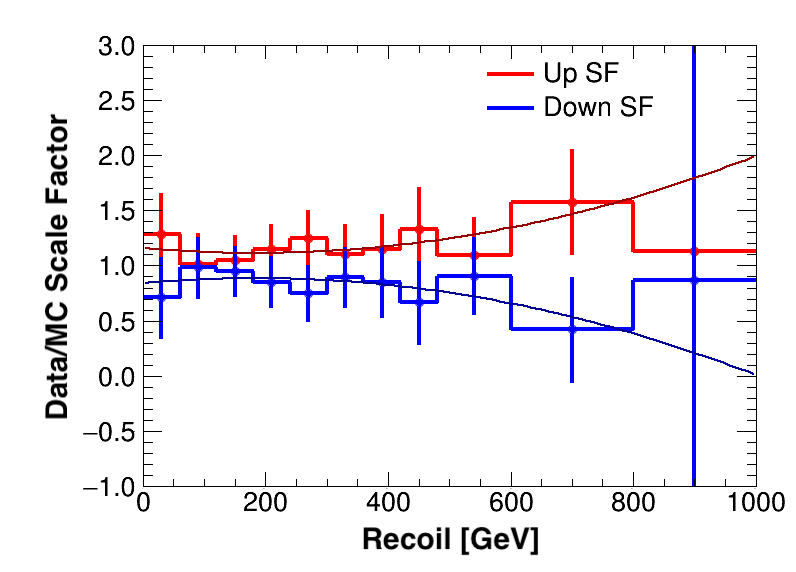
\includegraphics[width=0.6\textwidth]{figs/RecoilUpFit.png}
    \caption{The fake \ptmiss uncertainty at one standard deviation from the nominal recoil distribution as derived in simulation using Z bosons decaying to dielectrons and dimuons with $\mttll > 110\:\GeV$. In order to smoothen out the binned uncertainty, it is fit with a second-order polynomial.}
    \label{fig:recoilSF}
  \end{figure}

    \begin{figure}[h]
      \centering
      \subfloat[][DY, high \mttll-SF]{\label{subfig:DYfake}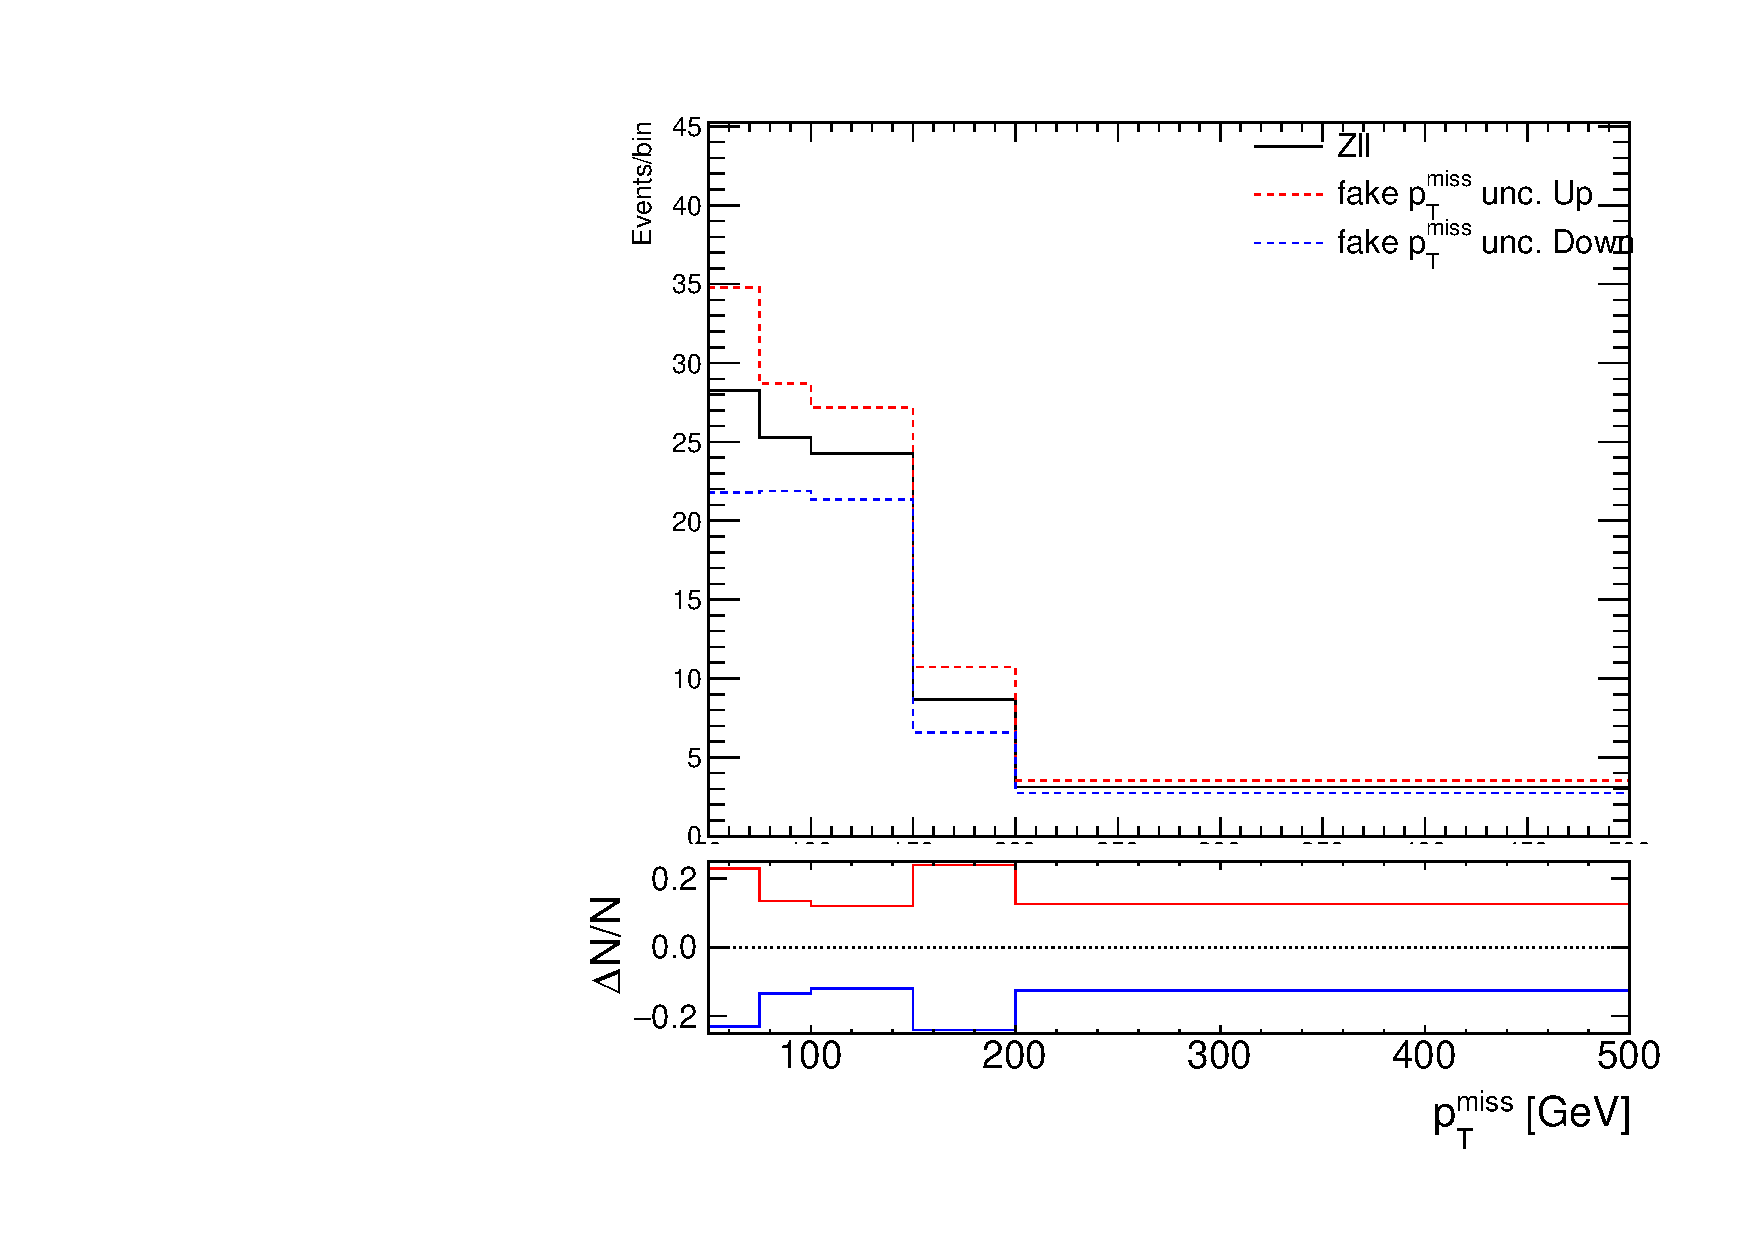
\includegraphics[width=0.48\textwidth]{systs/shapes_ttdm805101_sf_hi/Zll_RecoilCorr}}
      \subfloat[][\ttll, high \mttll-SF]{\label{subfig:tt2lfake}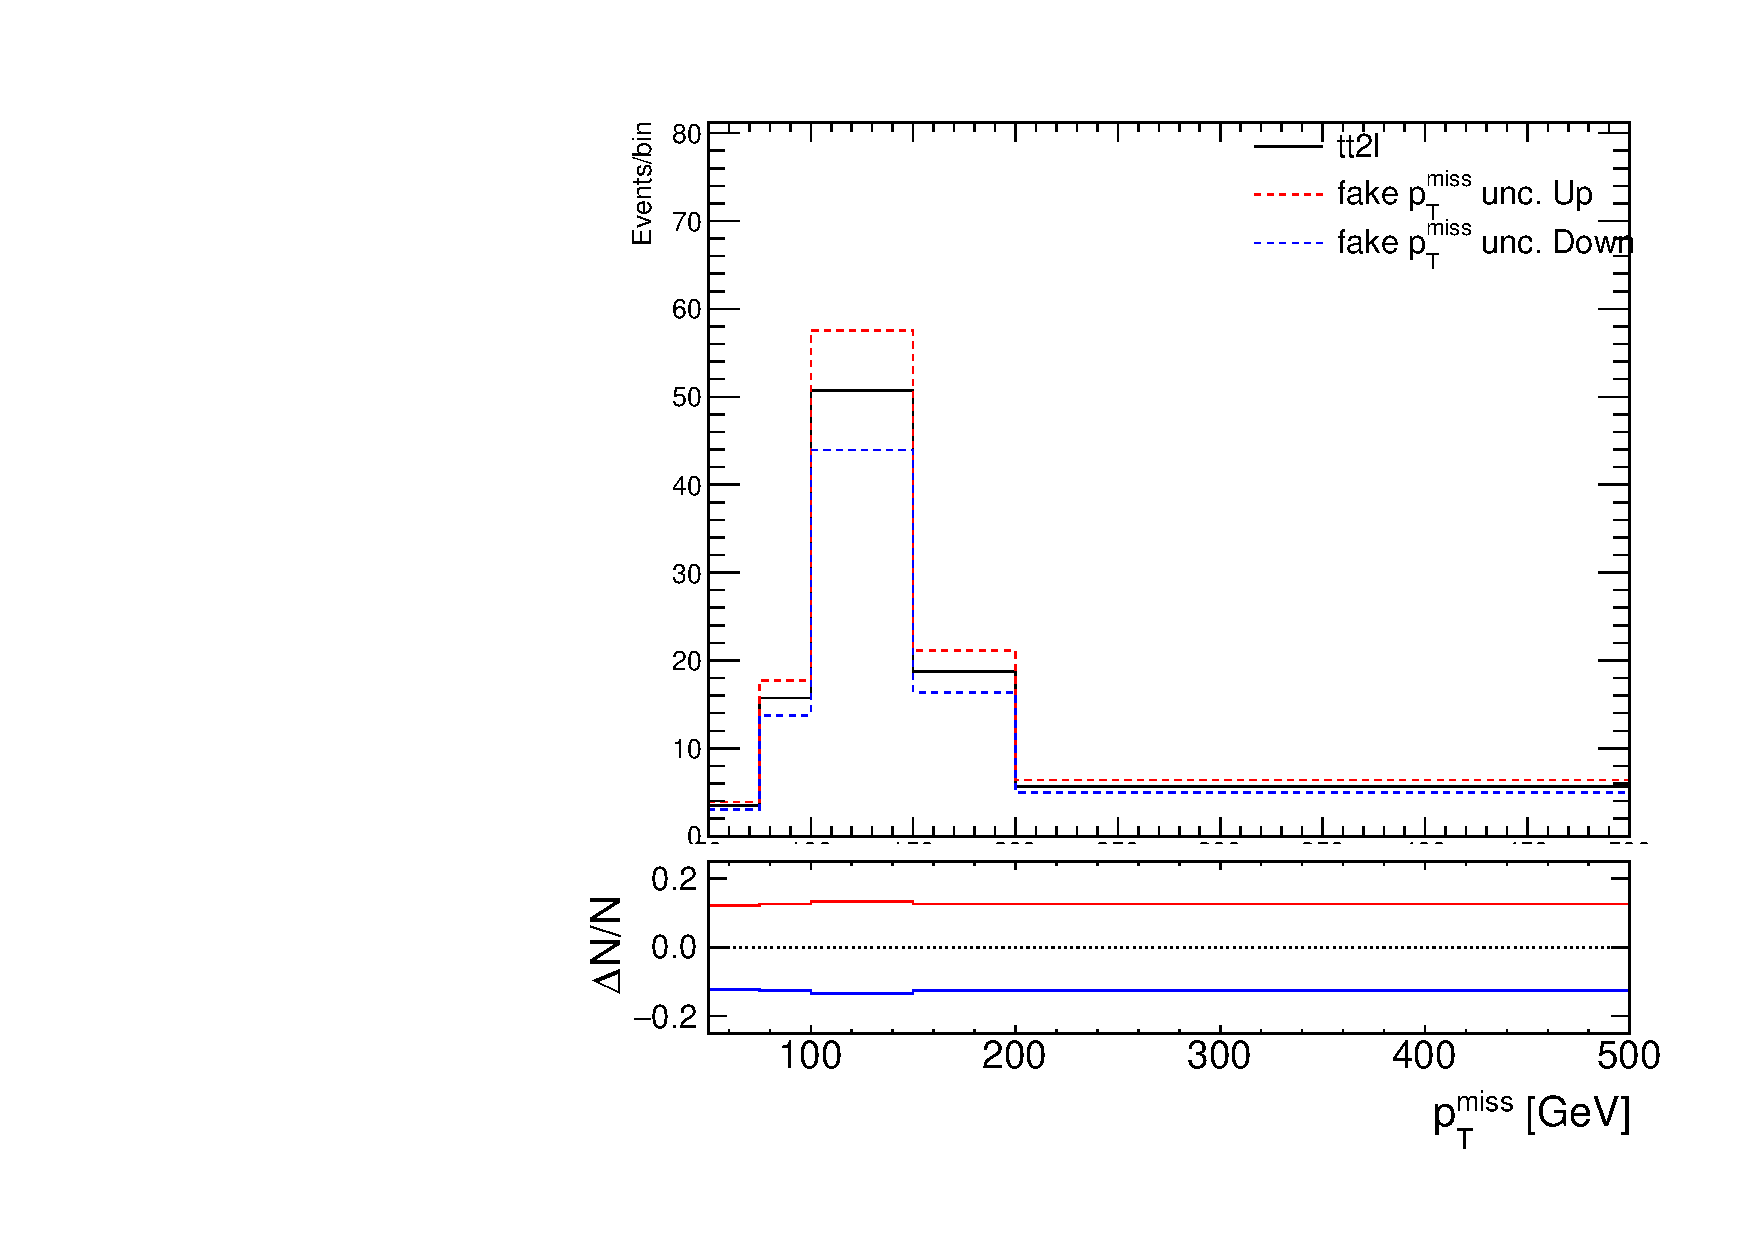
\includegraphics[width=0.48\textwidth]{systs/shapes_ttdm805101_sf_hi/tt2l_RecoilCorr}}
      \caption{The variation in the \ptmiss spectra for~\protect\subref{subfig:DYfake} DY and~\protect\subref{subfig:tt2lfake} \ttll in the high \mttll-SF SRs due to the variation of the fake \ptmiss uncertainty by $+1\sigma$ (red) and $-1\sigma$ (blue). The normalized residuals of the ``up'' and ``down'' shapes are shown in the lower panel.}
      \label{fig:fakeMETshape}
    \end{figure}

\item \textbf{Factorization and renormalization scales}:
In order to estimate the effects incurred from missing corrections from higher order perturbative QCD calculations for background processes, the renormalization scale, $\mu_R$, and the factorization scale, $\mu_F$, employed in the simulation matrix-element generator are halved or doubled independently~\cite{Collins:1989gx}, and the changes are propagated to the \ptmiss templates. The variation also covers the uncertainty in the finite order QCD calculations which are reliant on the scale choice as well. This is accommodated via weights obtained directly from the generator information in the MC simulation where available. The uncertainty is considered to be uncorrelated among the different background processes. 

\item \textbf{Top quark \pt reweighting}: 
The top quark \pt spectrum as measured in differential top quark pair production is observed to be softer than that of simulation, as discussed in \SectionRef{subsec:toppt}. In order to cover this effect, the scale factors derived in previous CMS measurements~\cite{Khachatryan:2016mnb} are applied to the \ttbar simulation by default. The uncertainty is estimated from a comparison of the top \pt spectrum obtained without the reweighting applied.
\item \textbf{Parton distribution function (PDF)}: Uncertainties due to the choice of PDF used to simulate the hard scatter process are estimated by reweighting the simulation samples with the ensemble of 100 PDF replicas~\cite{0954-3899-43-2-023001} provided by NNPDF3.0~\cite{Ball:2014uwa}.
\end{itemize}


\section{Statistical analysis}
\label{sec:stats}
The methods by which the statistical analysis is performed are outlined in the following section. A brief description of the model parameter estimation and statistical model inference methods are outlined. Finally, the means by which the signal is extracted is described. An in-depth discussion of statistical methods can be found in Ref.~\cite{Lista:2016chp}. 

\subsection{Maximum likelihood}
\label{subsec:maxlikelihood}
The maximum likelihood estimates the best value of the parameters (i.e. signal strength and background shape and normalizations), for which the observed data has the highest probability of estimating the true parameter value according to the hypothesis model. Following the discussion in~\cite{Lista:2016chp}, supposing in a set of $N$ events, we observe a set of measured quanties, $\bar{x}$. In the space of these observables we can define a set of bins, $n_{bin}$, and it is assumed that the number of events $n_{i}$ in each bin $i$ are Poisson-distributed such that,

\begin{equation}
  \mathcal{P}(n_{i}\mid\lambda_{i}) = \frac{\lambda_{i}^{n_{i}}e^{-\lambda_{i}}}{n_{i}!},
\end{equation}

where $\lambda_{i}$ is the number of expected events in the bin containing contributions from both signal and background processes such that $\lambda = \mu s + b$. The number of signal (background) events is denoted by $s$ ($b$), and subsequently the parameter $\mu$ represents the signal strength scaling, where $\mu=0$ corresponds to the background-only hypothesis, and $\mu=1$ is the nominal signal hypothesis. The likelihood function is then simply the product of Poisson probabilities for all bins,

\begin{equation}
  \mathcal{L} = \prod_{j=1}^{N}\frac{(\mu s_{j}+b_{j})^{n_j}}{n_{j}!}e^{-(\mu s_j + b_j)},
  \label{eq:like}
\end{equation}

where the mean number of entries in the $j$th bin from signal and background are

\begin{equation}
  s_{j}  = s_{\textrm{tot}}\int_{\textrm{bin j}} f_{s}(x;\textbf{\theta}_{s})dx, 
\label{eq:sigpdf}
\end{equation}

\begin{equation}
  b_{j}  = b_{\textrm{tot}}\int_{\textrm{bin j}} f_{b}(x;\textbf{\theta}_{b})dx. 
\label{eq:bkgpdf}
\end{equation}

The functions $f_{s}(x;\textbf{\theta}_{s})$ and $f_{b}(x;\textbf{\theta}_{b})$ are the $pdf$s of the variable $x$ for signal and background events and $\textbf{\theta}_s$ and $\textbf{\theta}_b$ are the nuisance parameters described in \SectionRef{sec:systunc}, which characterize the shape of the $pdf$s. The integrals in Eq.~\ref{eq:sigpdf} and Eq.~\ref{eq:bkgpdf} represent the probabilities for an event to be found in bin $j$, and $s_\mathrm{tot}$ and $b_\mathrm{tot}$ denote the total mean numbers of signal and background events, respectively. It is then clear that the likelihood in Eq.~\ref{eq:like} is a function of the nuisance parameters, $\mathcal{L}(\textbf{\theta})$, and the values of $\textbf{\theta}$ which maximize this quantity are said to fit the observation best.

\subsection{Hypothesis testing}
\label{subsec:hypothesis}

In order to determine whether to accept or reject a model depending on the outcome of a measurement, a frequentist test of a hypothesis is performed. In this case, we test the hypothesized value of the signal strength, $\mu$, which is interpreted as the ratio of the measured cross section, $\sigma$, to the predicted value from the theory model, $\sigma_{\textrm{TH}}$, such that $\mu=\frac{\sigma}{\sigma_{\textrm{TH}}}$. Hence, a null value of $\mu$ corresponds to an observation compatible with the SM background-only hypothesis, whereas if the observation is compatible with signal events as predicted by the model cross section, then $\mu=1$. 

Quantifying the level of agreement between the observation and a tested hypothesis is done via a test statistic $q(\mu)$, which is defined as the ratio of maximum likelihoods,

\begin{equation}
  q(\mu) = \frac{\mathcal{L}(\mathcal{D}\mid\mu,\hat{\hat{\textbf{\theta}}}(\mu))}{\mathcal{L}(\mathcal{D}\mid\hat{\mu},\hat{\textbf{\theta}})}
  \label{eq:proflikelihood}
\end{equation}

where the $\hat{\hat{\textbf{\theta}}}(\mu)$ indicates the values of the profiled nuisance parameters $\textbf{\theta}$, which maximize $\mathcal{L}$ for a fixed value of $\mu$, the dataset $\mathcal{D}$, and global observables. The denominator of the so-called \textit{profile likelihood ratio} defined by Eq.~\ref{eq:proflikelihood} is the value of $\mathcal{L}$ when evaluated with the maximum likelihood estimators (MLEs) $\hat{\mu}$ and $\hat{\textbf{\theta}}$. The MLEs and profiled nuisance parameters can analogously minimize the quantity $-2\ln{\mathcal{L}}$, so it is common to write the definition of the test statistic as,

\begin{equation}
   q(\mu) = -2\ln{\frac{\mathcal{L}(\mu,\hat{\hat{\textbf{\theta}}}(\mu))}{\mathcal{L}(\hat{\mu},\hat{\textbf{\theta}})}}, \mu' \leq \mu.
   \label{eq:likelihood}
\end{equation}

For the purposes of setting limits on theoretical parameters (i.e. determining the values of the parameters that are allowed or excluded given the available data) the test statistic $q(\mu)$ is used to discriminate between the hypothesis of the signal being produced at a rate $\mu$ from an alternative hypothesis of signal events being produced at a lesser rate $\mu' < \mu$. Thus, it is a test statistic for a one-sided alternative or moreover provides a one-sided upper limit. If the experiment were to be repeated multiple times, $q(\mu)$ would take on different values, thus the test statistic itself has a particular probability density function, $f(q(\mu)\mid H)$, dependent on the particular hypothesis, $H$, being tested. Then the probability that a given $q(\mu)_{\textrm{obs}}$ is an equal or more ``extreme'' outcome than observed, assuming $H$ is,

\begin{equation}
  p = \int_{q(\mu)_{\textrm{obs}}}^{\infty} f(q(\mu)\mid H)\xspace dq(\mu).
\label{eq:pvalue}
\end{equation}

The quantity in Eq.~\ref{eq:pvalue} and visualized in \FigureRef{fig:pvalues}, known as the \textit{p-value}, indicates a worse agreement with the corresponding $H$ for small $p$-values. In the language of discovery in high energy physics, it is customary to relate the $p$-value into a quantile of a unit Gaussian to express the significance $Z$, as shown in \FigureRef{fig:pvalues}. The area of the tail starting at an upward fluctuation of $Z$ standard deviations from the mean of the Gaussian random variable, should be equal to the $p$-value. The transformation is defined formally as, 

\begin{equation}
  Z = \Phi^{-1}(1-p)
\end{equation}

where $\Phi^{-1}$ is the inverse of the cumulative distribution of the single sided standard Gaussian. A $5\sigma$ significance is the standard requirement in experimental particle physics to claim a discovery, which is analogous to a $p$-value of $2.87 \times 10^{-7}$.

\begin{figure}
  \subfloat[][]{\label{subfig:pvalue}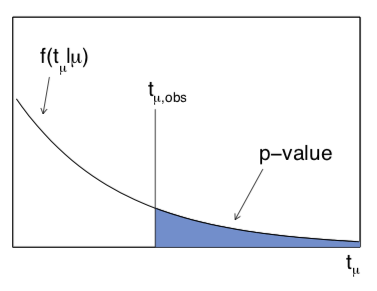
\includegraphics[width=0.4\textwidth]{figs/pvalue.png}}
  \subfloat[][]{\label{subfig:sig}   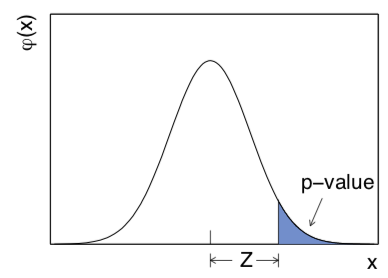
\includegraphics[width=0.4\textwidth]{figs/significance.png}}
  \caption{A visualization of the relation~\protect\subref{subfig:pvalue} between the observed value of the test statistic $q(\mu)_{\textrm{obs}}$, the probability density function $f(q(\mu)\mid H)$ and the $p$-value, and~\protect\subref{subfig:sig} between the $p$-value and the signficance $Z$.}
  \label{fig:pvalues}
\end{figure}

In the absence of a discovery, such that the $p$-value determined from the observed data cannot exclude the background-only hypothesis, the upper limit on the signal strength parameter, $\mu$, is established. The one-sided modified frequentist confidence level ($\textrm{CL}_s$) upper limit on $\mu$ is defined as,

\begin{equation}
  \textrm{CL}_{s} = \frac{p_\mu}{1-p_0}
  \label{eq:CLs}
\end{equation} 

where $p_{0}$ is the $p$-value determined given that the hypothesis under test is that of the SM background-only. In practice, results are calculated at $95\%$ $\textrm{CL}_s$ which is defined as the $\mu$ that produces $\textrm{CL}_s=0.05$.

\subsection{Signal extraction}
\label{subsec:signal}

In order to extract the results, a binned maximum likelihood fit is performed simultaneously on the \ptmiss distributions in the SRs as defined in more detail in \SectionRef{sec:observables}. A single strength parameter is used to scale the signal across all the SRs. The sources of systematic uncertainties are represented by nuisance parameters in the fit, as described in greater detail in \SectionRef{sec:systunc}.

The likelihood ratio defined by Eq.~\ref{eq:likelihood} is used to assess the fit for the saturated model, and provides a generalization of the $\chi^2$ goodness-of-fit test as per~\cite{BAKER1984437}. The fitted background-only \ptmiss distributions are shown in~\FigureRef{fig:postfit_lo} and~\FigureRef{fig:postfit_hi}. The corresponding observed data yield and post-fit SM background expected yields are presented for the high and low purity categories in \TableRef{tab:cat-hi_postfit_yields} and~\ref{tab:cat-lo_postfit_yields}, respectively. The $p$-value of 0.06, as defined by Eq.~\ref{eq:pvalue}, is determined from the distribution of the likelihood ratio obtained from pseudodata generated from the fitted simulation yields. No significant excess in the SRs is observed. 

\begin{table}[!htbp]
\caption{Background-only post-fit event yields passing selection in the $\mttll>110\:\GeV$ (high signal purity) category. The expected (pre-fit) yield is also shown for a pseudoscalar $m_a=100\:\GeV,\,\mDM=1\:\GeV$ signal. The uncertainties include contributions from both systematic and statistical sources.}
\label{tab:cat-hi_postfit_yields}
\centering
\begin{tabular}{l|r|r}
\hline
\multicolumn{3}{c}{\mttll$>110\:\GeV$} \\
\hline
                            & \multicolumn{1}{c|}{$ee+\mu\mu$} & \multicolumn{1}{c}{$e\mu$} \\
\hline
  Diboson                   &  $3.83 \pm   0.51$        &  $1.42 \pm   0.58$          \\
  Drell-Yan                 &  $68.51 \pm   9.88$       &  $0.85 \pm   0.51$          \\
  Single t ($2\ell$)        &  $7.34 \pm   1.51$        &  $8.59 \pm   1.88$          \\
  $\ttbar+V$                &  $7.83 \pm   1.12$        &  $5.87 \pm   0.95$          \\
  $\ttbar(2\ell)$           &  $77.67 \pm   5.60$       &  $104.91 \pm 7.49$          \\
  Fakes                     &  $0.72 \pm   0.92$        &  $4.14 \pm   2.82$          \\
\hline
  SM Expected               & $165.90 \pm 10.26$        & $125.77 \pm 8.96$            \\
  Observed                  & $156$                     & $128$                        \\
  $m_a=100,\,m_\chi=1$      & $5.18 \pm  0.089$         & $5.82 \pm  0.094$            \\
\hline
\end{tabular}
\end{table}

\begin{table}[!htbp]
\caption{Background-only post-fit event yields passing selection in the $\mttll<110\:\GeV$ (low signal purity) category. The expected (pre-fit) yield is also shown for a pseudoscalar $m_a=100\:\GeV,\,\mDM=1\:\GeV$ signal. The uncertainties include contributions from both systematic and statistical sources.}
\label{tab:cat-lo_postfit_yields}
\centering
\begin{tabular}{l|r|r}
\hline
\multicolumn{3}{c}{\mttll$<110\:\GeV$} \\
\hline
                           & \multicolumn{1}{c|}{$ee + \mu\mu$} & \multicolumn{1}{c}{$e\mu$} \\
\hline
  Diboson                  &  $178.05 \pm  10.85$     &    $148.68 \pm   9.19$     \\
  Drell-Yan                &  $2633.18 \pm 279.35$    &    $267.71 \pm  29.52$     \\
  Single t ($2\ell$)       &  $3356.63 \pm 553.19$    &  $3946.44 \pm 648.20$    \\
  $\ttbar+V$               &  $232.94 \pm  31.56$     &   $256.39 \pm  33.33$     \\
  $\ttbar(2\ell)$          &  $79534.15 \pm 702.17$   & $94338.27 \pm 805.11$    \\
  Fakes                    &  $689.18 \pm 322.88$     &   $792.42 \pm  80.64$    \\
\hline
  SM Expected              & $86624.13 \pm 401.67$      & $ 99749.92 \pm 469.50$ \\
  Observed                 & $86619$                    & $99793$                \\
  $m_a=100,\,m_\chi=1$     & $19.63 \pm  0.17$          & $22.70 \pm  0.19$      \\
\hline
\end{tabular}
\end{table}

\begin{figure}
  \subfloat[][low purity, $ee+\mu\mu$ channel]{\label{subfig:postfit_lo_sf}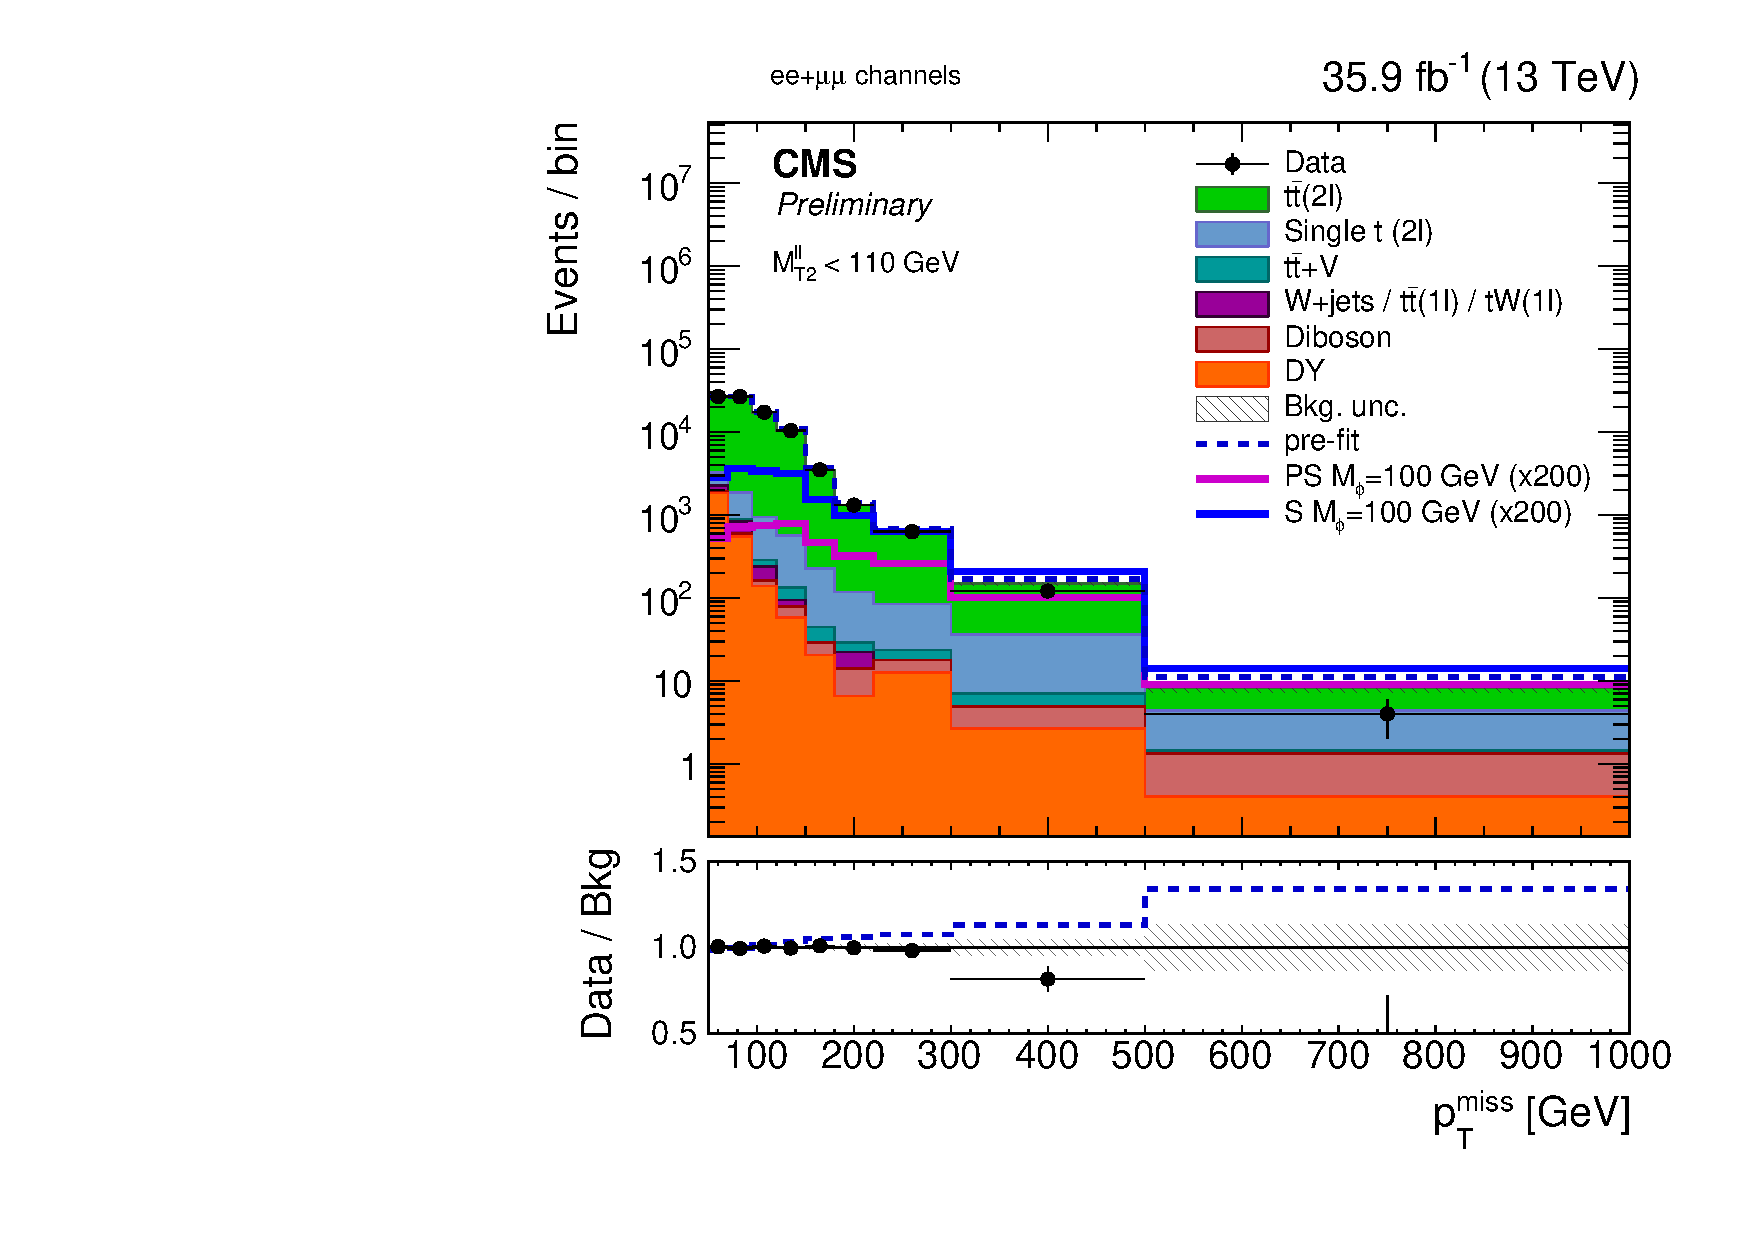
\includegraphics[width=0.48\textwidth]{figs/postfit/metlog_shapes_fit_b_dl_lo_mt2_ll.pdf}}
  \subfloat[][low purity, $e\mu$ channel]     {\label{subfig:postfit_lo_of}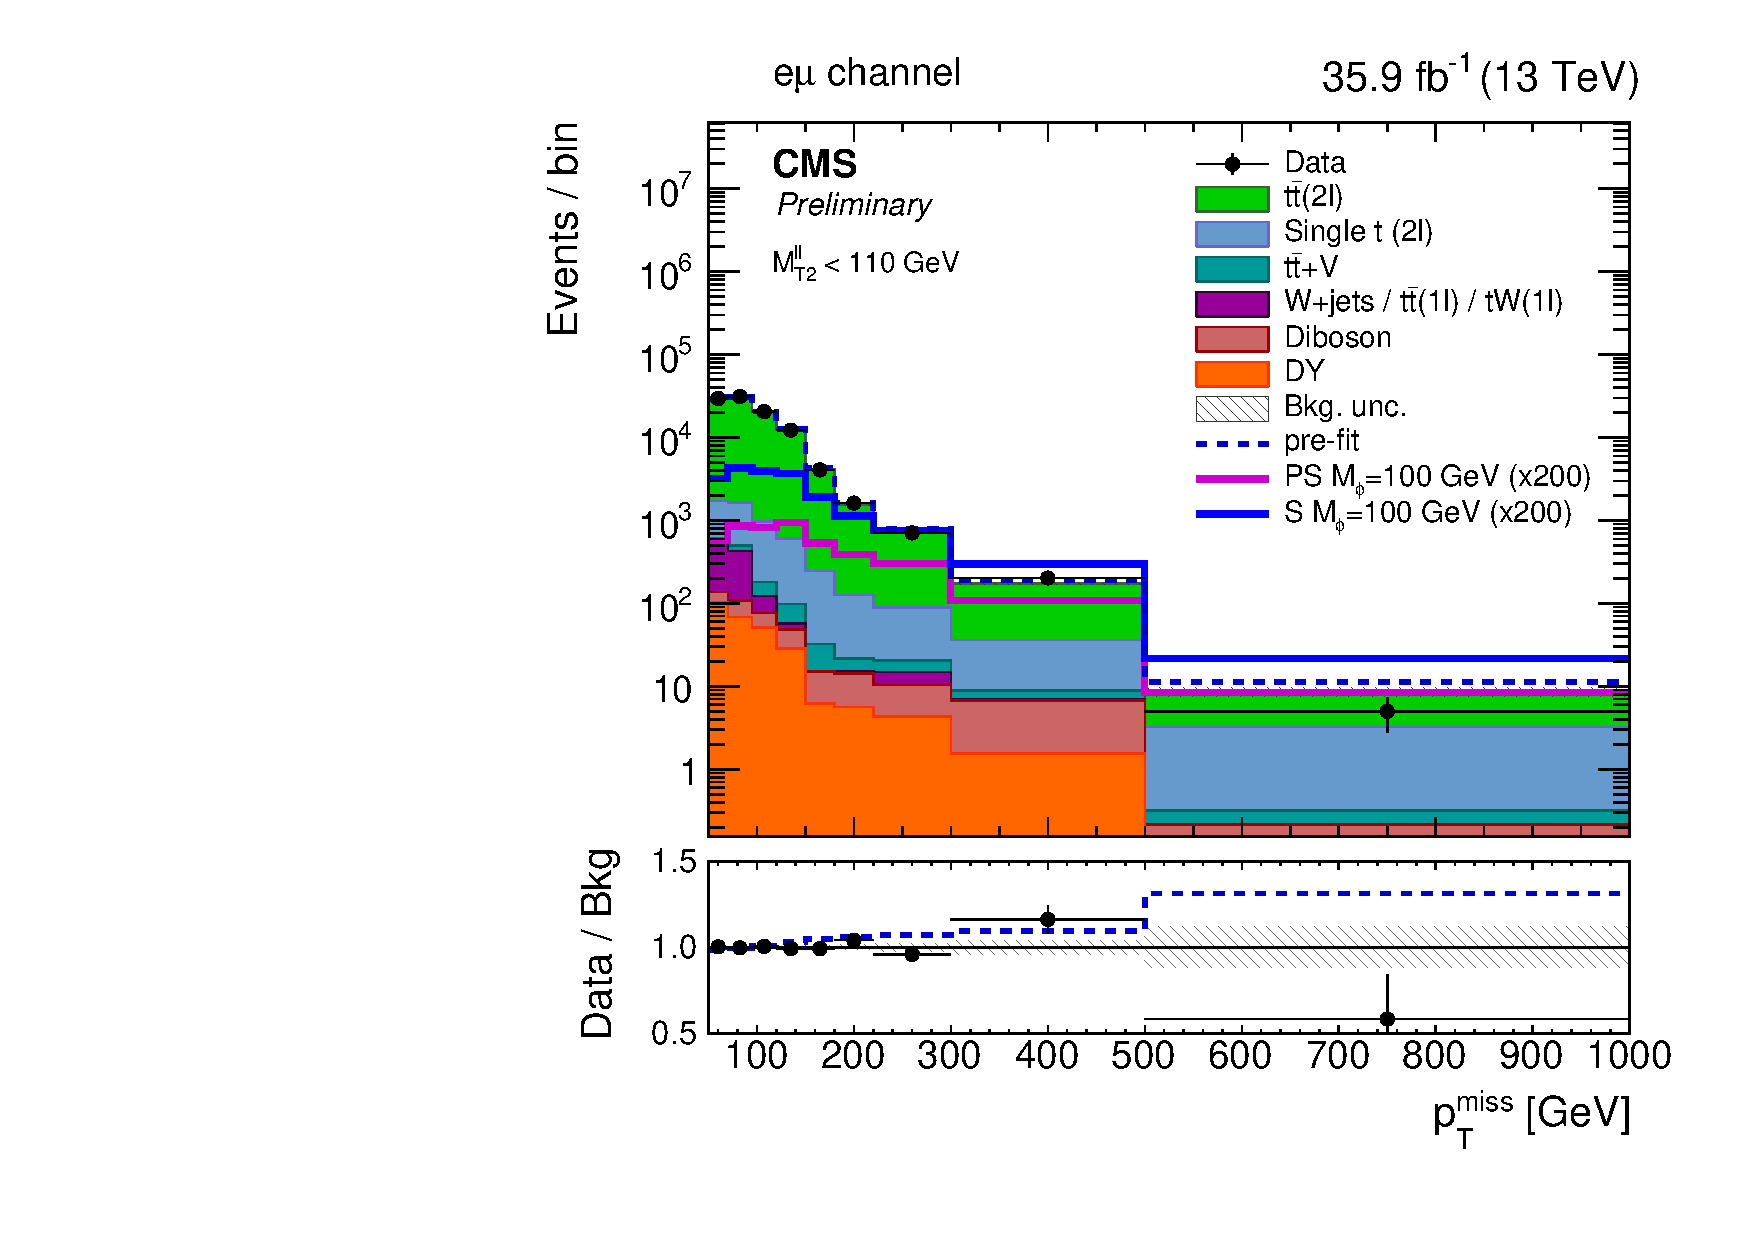
\includegraphics[width=0.48\textwidth]{figs/postfit/metlog_shapes_fit_b_dl_lo_mt2_em.pdf}}
  \caption{The background-only post-fit \ptmiss distributions in the low signal purity SRs. The expected (pre-fit) \ptmiss distributions for two example signals (scalar and pseuscalar mediator, $m_{\phi/a}=100\:\GeV$) with $\mDM=1\:\GeV$ are scaled up by a factor of 200. The dashed blue line represents the total expected (pre-fit) MC background \ptmiss shape, and the subsequent ratio between the pre-fit and post-fit shape in the lower ratio panel. The last bin of the distributions includes overflow. Statistical and systematic uncertainties are shown.}
  \label{fig:postfit_lo}
\end{figure}

\begin{figure}
  \subfloat[][high purity, $ee+\mu\mu$ channel]{\label{subfig:postfit_hi_sf}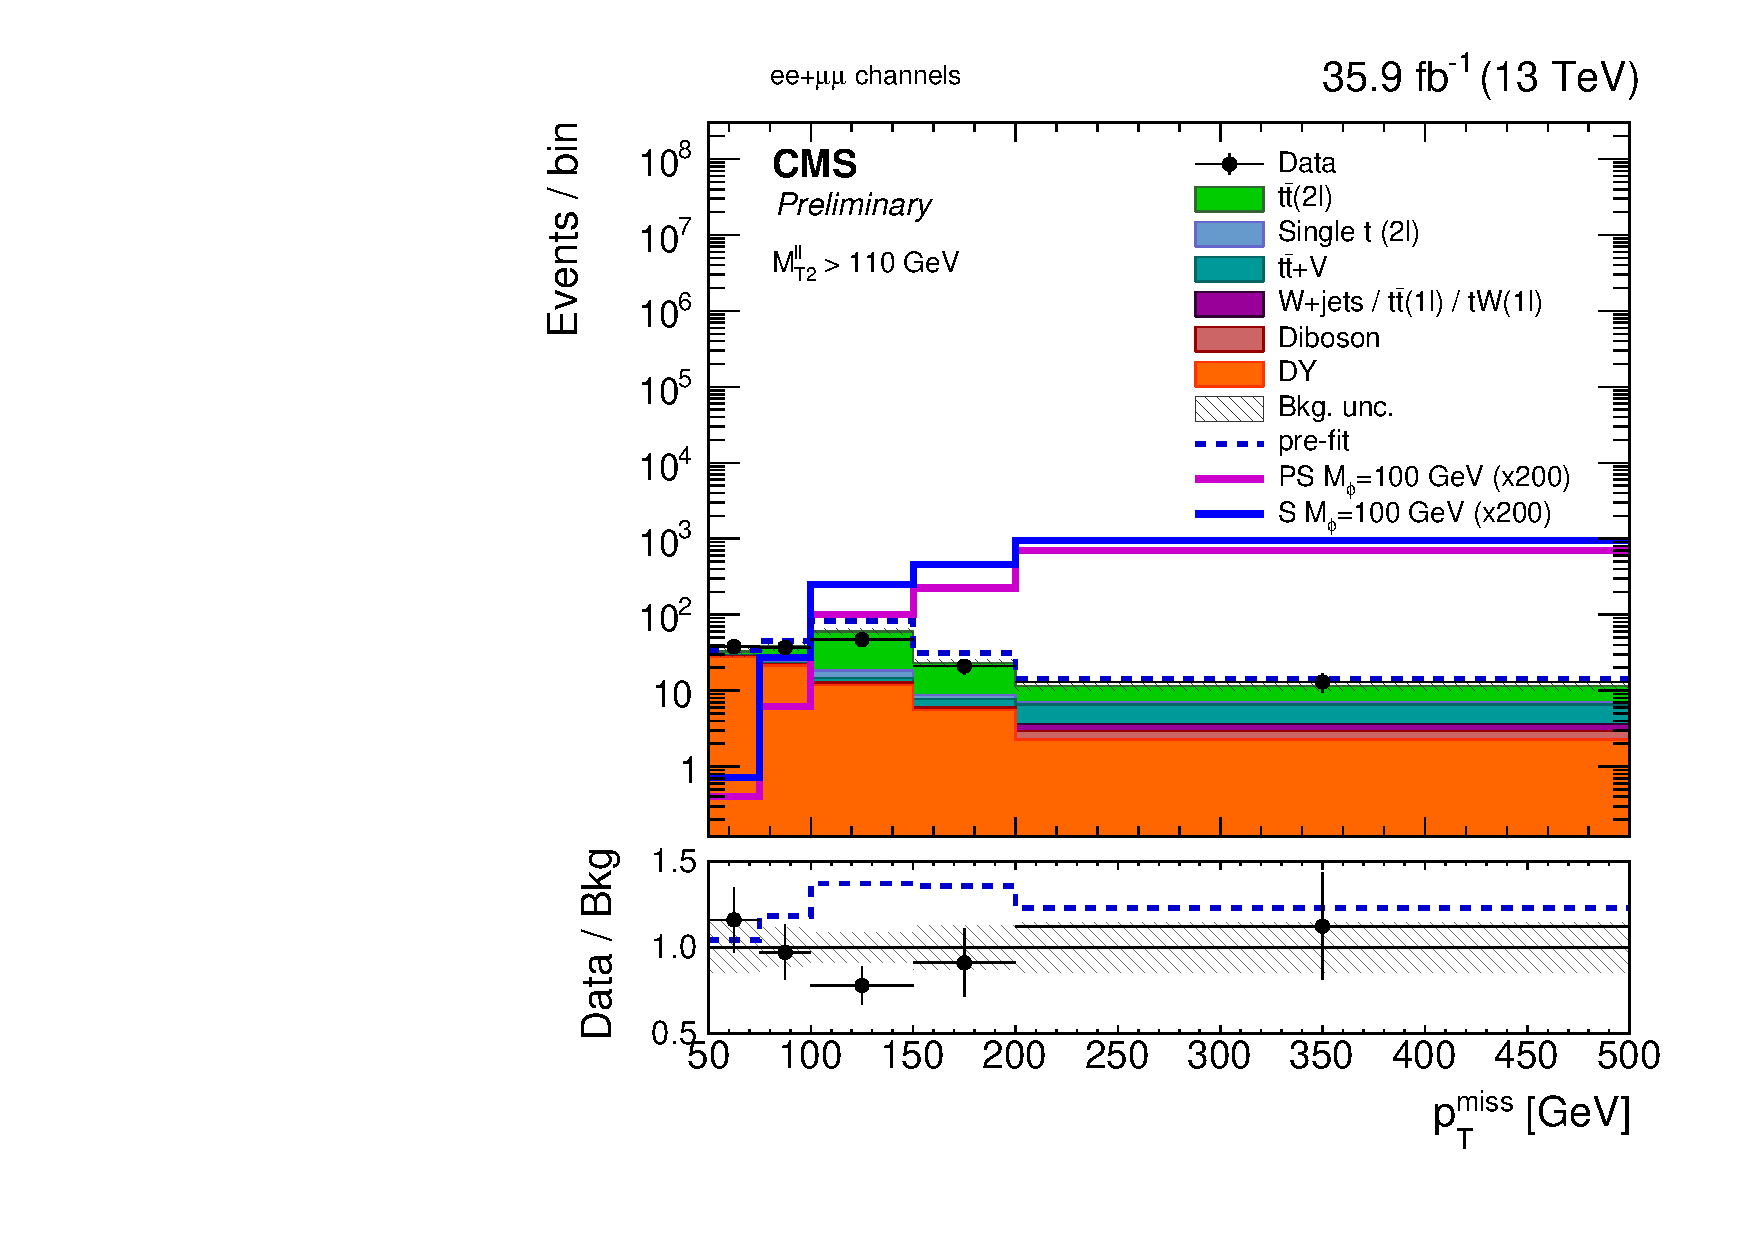
\includegraphics[width=0.48\textwidth]{figs/postfit/metlog_shapes_fit_b_dl_hi_mt2_ll.pdf}}
  \subfloat[][high purity, $e\mu$ channel]     {\label{subfig:postfit_hi_of}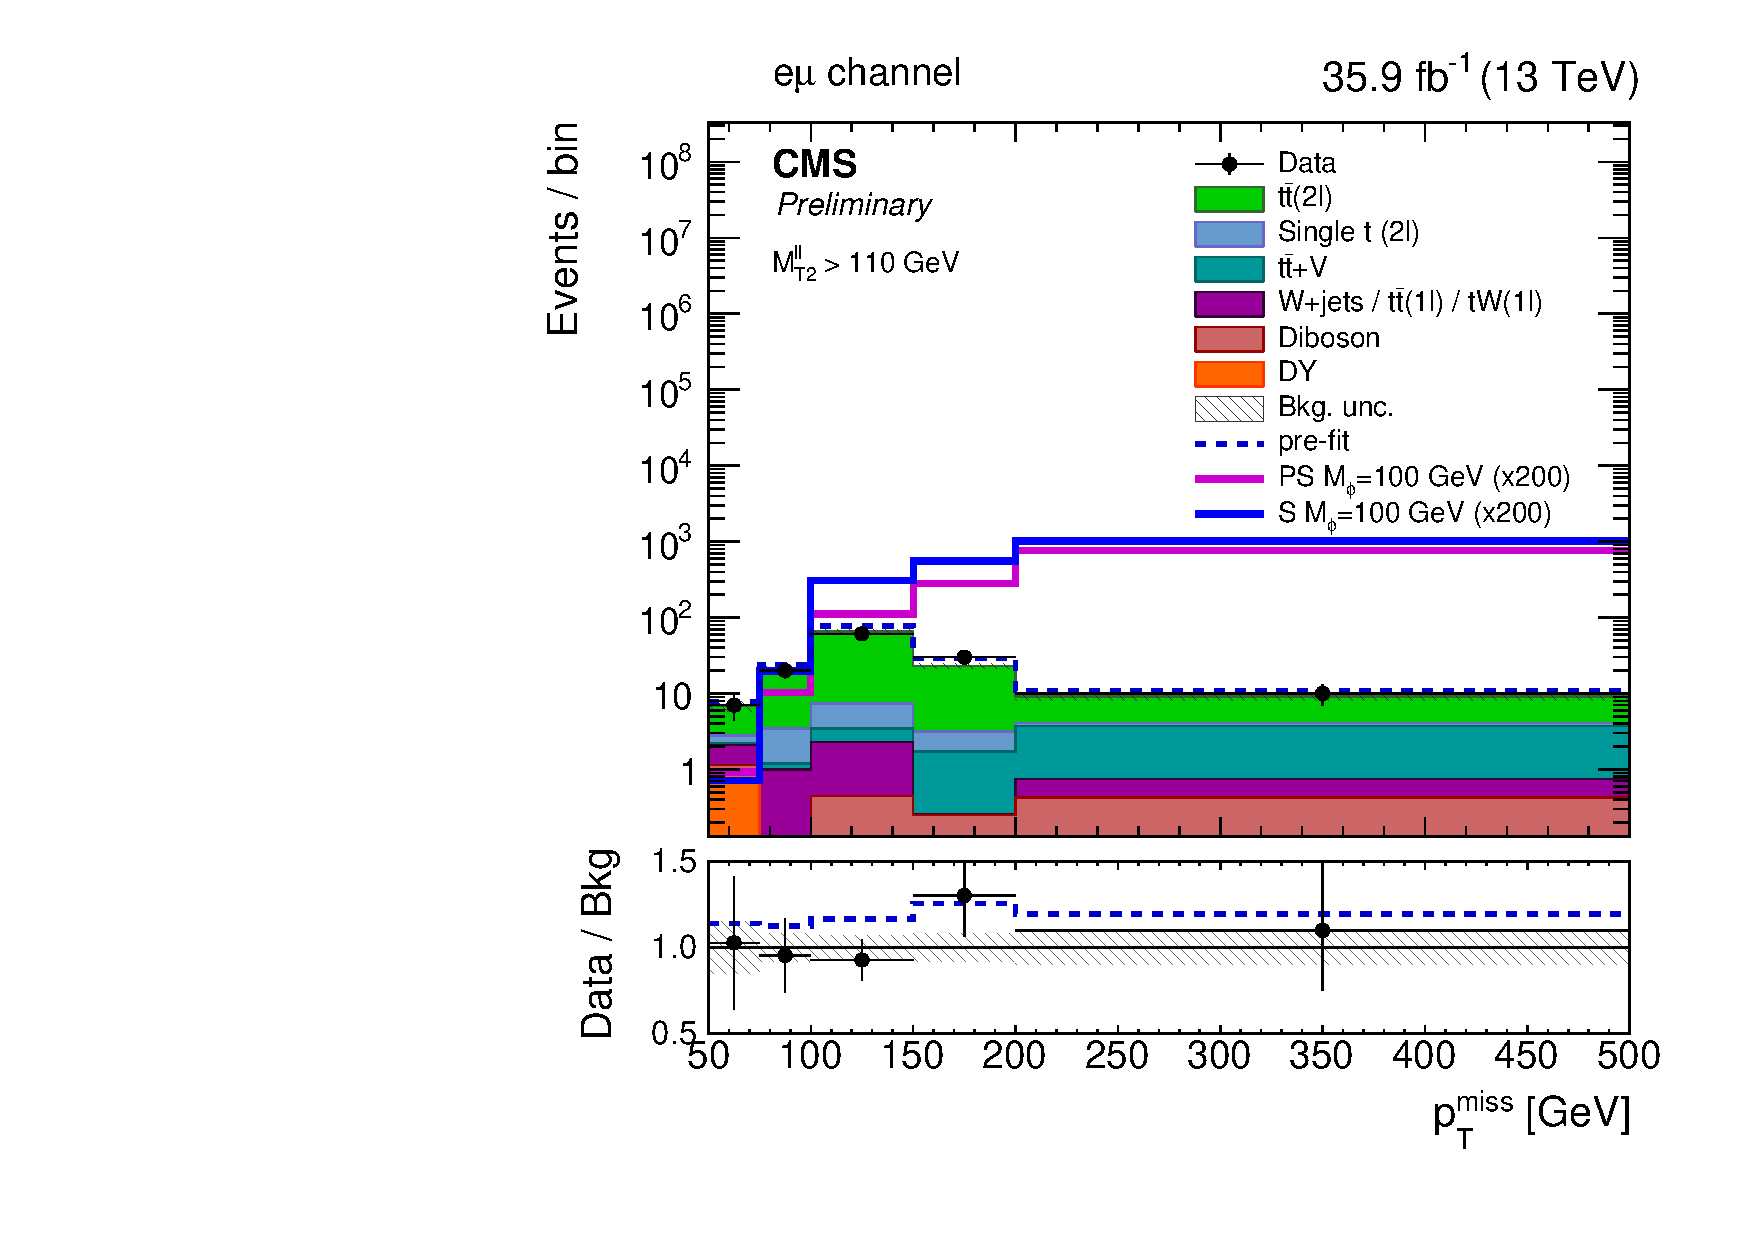
\includegraphics[width=0.48\textwidth]{figs/postfit/metlog_shapes_fit_b_dl_hi_mt2_em.pdf}}
  \caption{The background-only post-fit \ptmiss distributions in the high signal purity SRs. The pre-fit \ptmiss distributions for two example signals (scalar and pseuscalar mediator, $m_{\phi/a}=100\:\GeV$) with $m_{\chi}=1\:\GeV$ are scaled up by a factor of 200. The dashed blue line represents the total expected (pre-fit) MC background \ptmiss shape, and the subsequent ratio between the pre-fit and post-fit shape in the lower ratio panel. The last bin of the distributions includes overflow. Statistical and systematic uncertainties are shown.}
  \label{fig:postfit_hi}
\end{figure}

\subsection{Post-fit diagnostics}

The observed \textit{pull} statistic in Eq.~\ref{eq:pulls} as defined in~\cite{Karbach:2012vg}, is used to assess whether the fit gives unbiased central values of the nuisance parameters and errors of correct coverage. The metric quantifies how far from the expected value, a nuisance parameter had to be ``pulled'' in order to find the maximum likelihood estimate. The pull is expected to follow a unit Gaussian, with a mean of 0 and unitary width.

\begin{equation}
  \textrm{pull}(\theta) = \frac{\theta^{\textrm{fit}}-\theta^{\textrm{true}}}{\sigma_{\theta^{\textrm{fit}}}}
  \label{eq:pulls}
\end{equation}

The \textit{impact} quantity~\cite{CYRSP303} is measured as a means to gauge how much the parameter of interest (POI), that being the signal strength parameter $\mu$, depends on changes in the nuisance parameters. The impact of a nuisance parameter is defined as,

\begin{equation}
  \textrm{Impact}(\theta) = \Delta\mu^{\pm} = \hat{\hat{\mu}}_{\theta^{\textrm{true}}\pm\sigma_{\theta}} - \hat{\mu},
  \label{eq:impact}
\end{equation}

where $\hat{\hat{\mu}}_{\theta^{\textrm{true}}\pm\sigma_{\theta}}$ is defined as the maximum likelihood estimator of $\mu$ when every nuisance parameter except $\theta$ is profiled, and $\theta$ is set to its expectation value ($\theta^{\textrm{true}}$) plus or minus one standard devation according to the post-fit uncertainty. The relative importance of the various systematic uncertainties are determined according to their impact on $\mu$, since not all nuisance parameters are of equal importance in the fitting procedure.

The pulls are computed for the nuisance parameters representing the systematic uncertainties defined in \SectionRef{sec:systunc}. \TableRef{tab:nuisancenames} relates the nuisance name as seen in the pulls plot in~\FigureRef{fig:pulls} to the corresponding systematic uncertainty. The table also summarizes which process is affected, and if the uncertainty affects the shape or normalization of a process. Unless indicated under the description heading, a nuisance is treated as correlated across both same and opposite flavor, high and low \mttll signal regions, and across the signal and all background processes. The pulls in~\FigureRef{fig:pulls} are computed considering the background-only hypothesis (red markers) and signal-plus-background hypothesis (blue markers), where the signal under consideration is a psuedoscalar mediator with $m_a=100\:\GeV$ and $\mDM=1\:\GeV$. None of the nuisances are pulled significantly relative to the a priori uncertainties (grey hatching). The most constrained nuisances are the JES (\texttt{CMS\_scale\_j}), constrained to 0.14 of the a priori value, and the renormalization/factorization scale uncertainty on the \ttll (\texttt{tt\_qcdScale}), constrained to the 0.27 of the a priori value. The level of constraint on the JES uncertainty is quite strong, but is not necessarily unwarranted or alarming for that matter. As given in \SectionRef{subsec:sources}, the procedure used to assess the effects of the JES uncertainty are such that the energy of the two or more required jets in an event is raised and lowered by the $1\sigma$ uncertainty coherently. The change in energy is propagated to the \MET to obtain the ``up'' and ``down'' \MET templates. Varying the energy in a correlated way where events can have a high jet multiplicity can yield large variations in the \MET. To this end, the uncertainty applied is not necessarily incorrect but is instead very convservative since it is unlikely that all the jet energies in an event are mismeasured in the same direction. In addition, the statistical power of the low \mttll region is quite significant, thus a conservative per-event uncertainty combined with a large sample size will unsurprisingly yield the level of constraint observed.

\begin{sidewaystable}
  \centering
  \scalebox{0.8}{
    \begin{tabular}{|l|r|c||c|c|c|c|c|c|c|}
      \hline
      Name                    & Description                                  & Type & Signal & \ttll & Single t ($2\ell$) & \ttbar+$V$ & Diboson & Drell-Yan & Fakes  \\
      \hline
      \texttt{CMS\_eff\_b}      & b-tagging efficiency                         & lnN  & \checkmark & \checkmark & \checkmark &  \checkmark &  \checkmark &  \checkmark &     \\
      \texttt{CMS\_eff\_e}      & electron reconstruction/selection efficiency & lnN  & \checkmark & \checkmark & \checkmark &  \checkmark &  \checkmark &  \checkmark &     \\
      \texttt{CMS\_eff\_m}      & muon reconstruction/selection efficiency     & lnN  & \checkmark & \checkmark & \checkmark &  \checkmark &  \checkmark &  \checkmark &     \\
      \texttt{CMS\_eff\_mistag} & b mistag rate                                & lnN  & \checkmark & \checkmark & \checkmark &  \checkmark &  \checkmark &  \checkmark &     \\
      \texttt{CMS\_norm\_ST}    & single top normalization                     & lnN  &            &            & \checkmark &             &             &             &     \\
      \texttt{CMS\_scale\_j}    & jet energy scale                             & shape& \checkmark & \checkmark & \checkmark &  \checkmark &  \checkmark &  \checkmark &     \\
      \texttt{CMS\_scale\_pu}   & pile up                                      & lnN  & \checkmark & \checkmark & \checkmark &  \checkmark &  \checkmark &  \checkmark &     \\
      \texttt{RecoilCorr}     & fake \ptmiss uncertainty (high \mttll)     & shape& \checkmark & \checkmark & \checkmark &  \checkmark &  \checkmark &  \checkmark &     \\
      \texttt{Zjets\_qcdScale} & factorization/renormalization uncertainty on DY & shape &        &          &         &             &             &  \checkmark      &     \\
      \texttt{hi\_ee\_Rinout}   & \Rinout uncertainty: high \mttll, $ee$ events    & lnN      &        &          &         &             &             &  \checkmark      &     \\
      \texttt{hi\_mm\_Rinout}   & \Rinout uncertainty: high \mttll, $\mu\mu$ events& lnN      &        &          &         &             &             &  \checkmark      &     \\
      \texttt{lo\_ee\_Rinout}   & \Rinout uncertainty: low \mttll, $ee$ events     & lnN      &        &          &         &             &             &  \checkmark      &     \\
      \texttt{lo\_mm\_Rinout}   & \Rinout uncertainty: low \mttll, $\mu\mu$ events & lnN      &        &          &         &             &             &  \checkmark      &     \\
      \texttt{hi\_ee\_fakes}    & fakes uncertainty: high \mttll, $ee$ events     & lnN      &        &          &         &             &             &                  & \checkmark     \\
      \texttt{hi\_em\_fakes}    & fakes uncertainty: high \mttll, $e\mu$ events   & lnN      &        &          &         &             &             &                  & \checkmark     \\
      \texttt{hi\_mm\_fakes}    & fakes uncertainty: high \mttll, $\mu\mu$ events & lnN      &        &          &         &             &             &                  & \checkmark     \\
      \texttt{lo\_ee\_fakes}    & fakes uncertainty: low \mttll, $ee$ events      & lnN      &        &          &         &             &             &                  & \checkmark     \\
      \texttt{lo\_em\_fakes}    & fakes uncertainty: low \mttll, $e\mu$ events    & lnN      &        &          &         &             &             &                  & \checkmark     \\
      \texttt{lo\_mm\_fakes}    & fakes uncertainty: low \mttll, $\mu\mu$ events  & lnN      &        &          &         &             &             &                  & \checkmark     \\
      \texttt{lumi\_13TeV}     & luminosity                                   & lnN      & \checkmark & \checkmark & \checkmark &  \checkmark &  \checkmark &  \checkmark &     \\
      \texttt{pdf}            & parton distribution function                 & shape    & \checkmark & \checkmark & \checkmark &  \checkmark &  \checkmark &  \checkmark &     \\
      \texttt{topPt}          & top \pt modeling                             & shape    &            & \checkmark &            &             &             &             &     \\
      \texttt{trigeff\_ll}     & dilepton trigger efficiency                  & lnN      & \checkmark & \checkmark & \checkmark &  \checkmark &  \checkmark &  \checkmark &     \\
      \texttt{ttV\_qcdScale}   & factorization/renormalization uncertainty on \ttbar+V & shape &            &            &            & \checkmark  &             &             &     \\
      \texttt{tt\_qcdScale}    & factorization/renormalization uncertainty on \ttll      & shape &            & \checkmark &            &             &             &             &     \\
      \hline
    \end{tabular}
  }
  \caption{A summary of the naming convention for the nuisance parameters used in the fit, whether each is implemented as ``lnN'' (normalization uncertainty) or ``shape'' (shape uncertainty), and which processes each affects. Unless indicated under the description heading, a nuisance is treated as correlated across both same and opposite flavor, high and low \mttll signal regions, and across the signal and all background processes.}
  \label{tab:nuisancenames}
\end{sidewaystable}

\begin{figure}
  \centering
  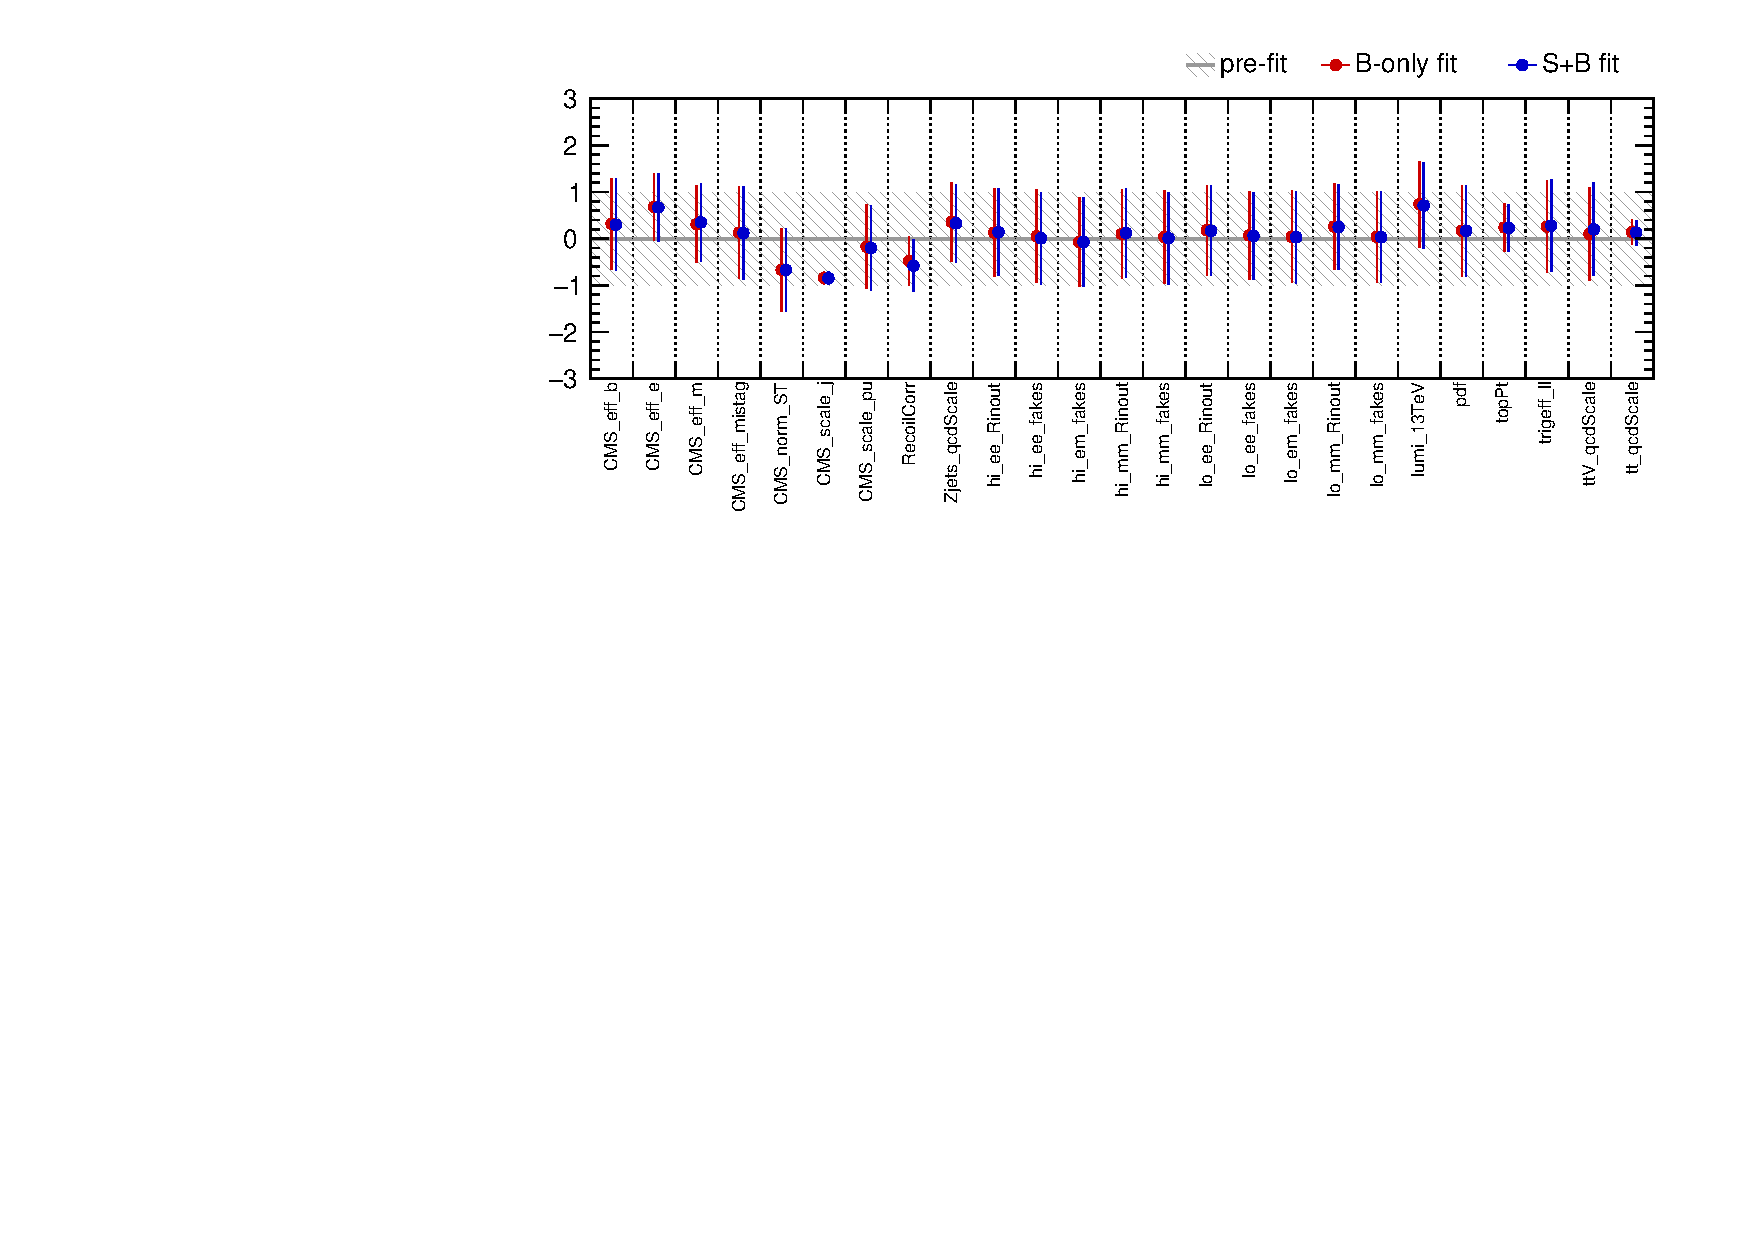
\includegraphics[width=\textwidth]{figs/pulls_35p9_ttdm8061001.pdf}
  \caption{Background-only (red) and signal-plus-background (blue) post-fit nuisance pulls.}
  \label{fig:pulls}
\end{figure}
